\documentclass{article}
\usepackage{parskip}
\usepackage{pdfpages}
\usepackage[margin=.6in]{geometry}
\begin{document}
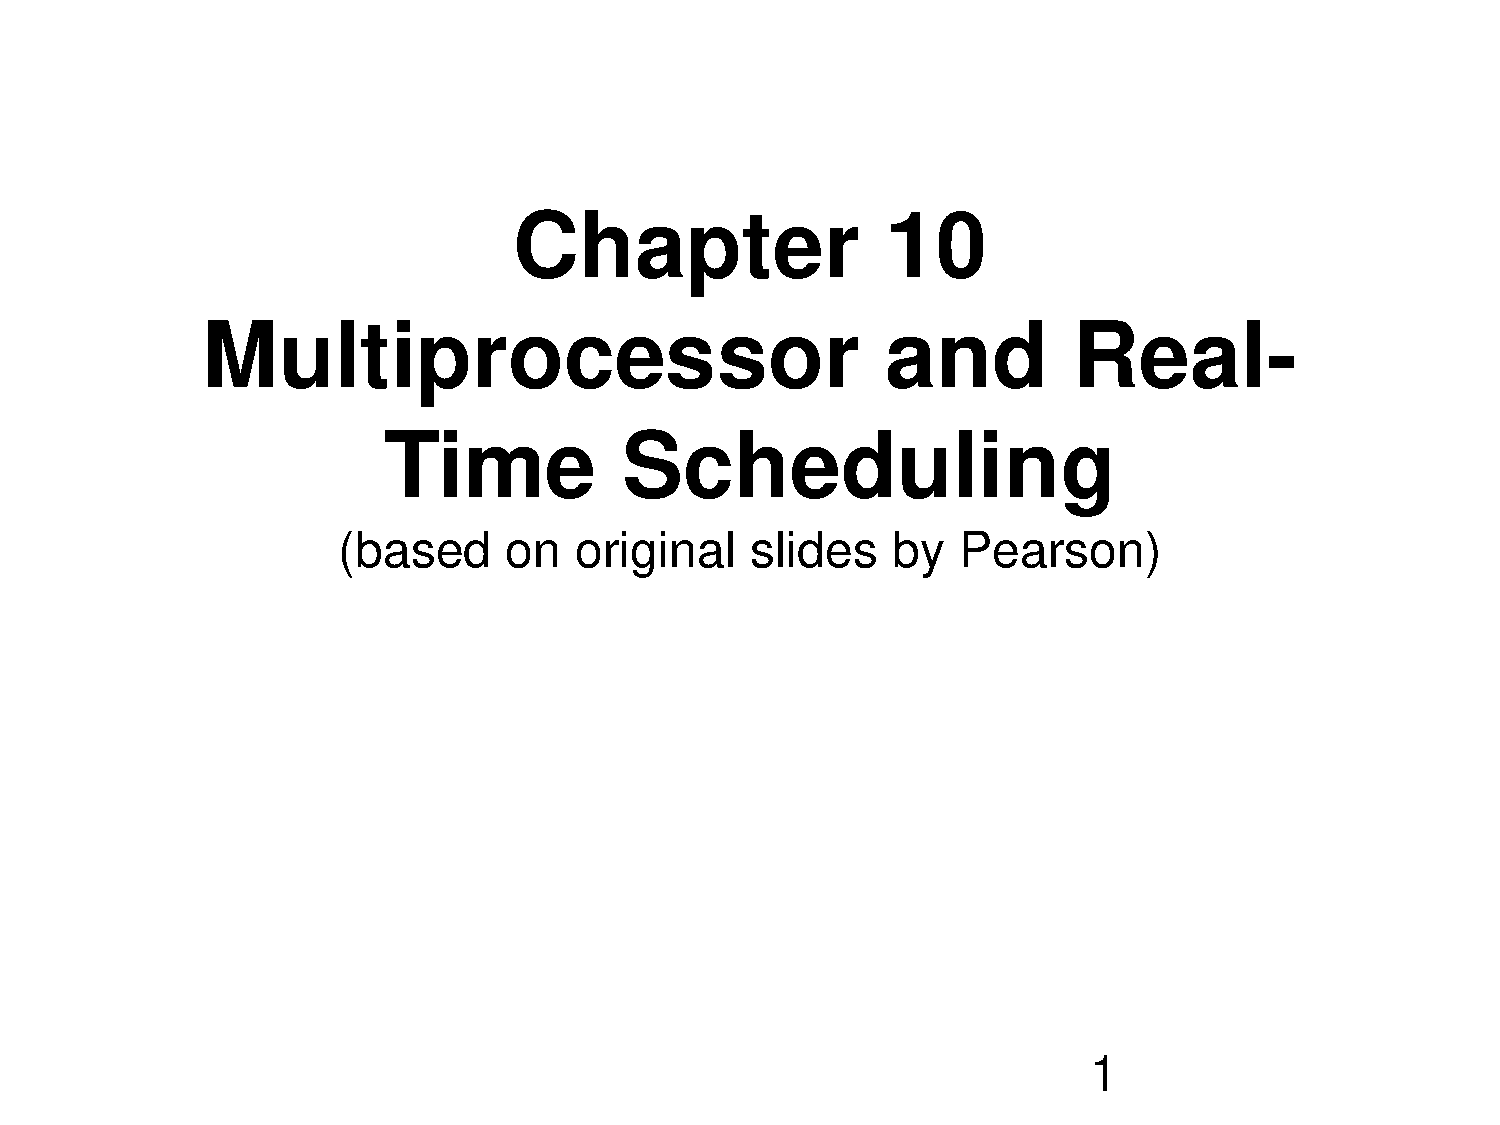
\includepdf[page=1]{10.pdf}
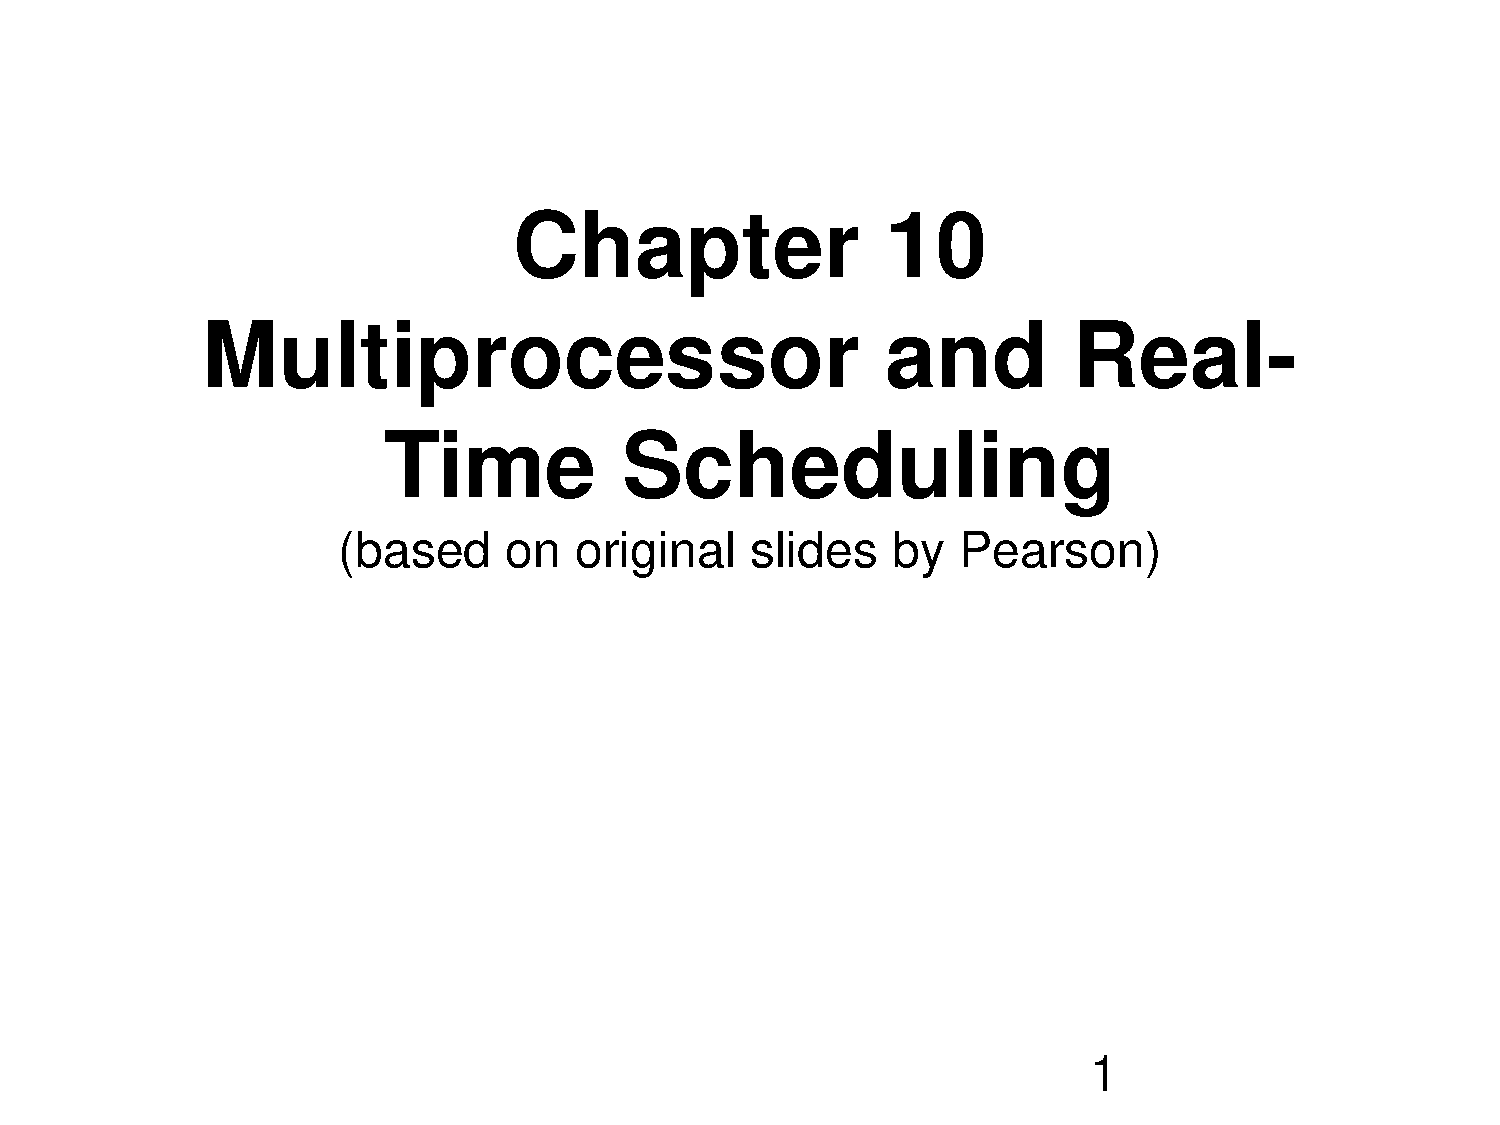
\includepdf[page=2]{10.pdf}
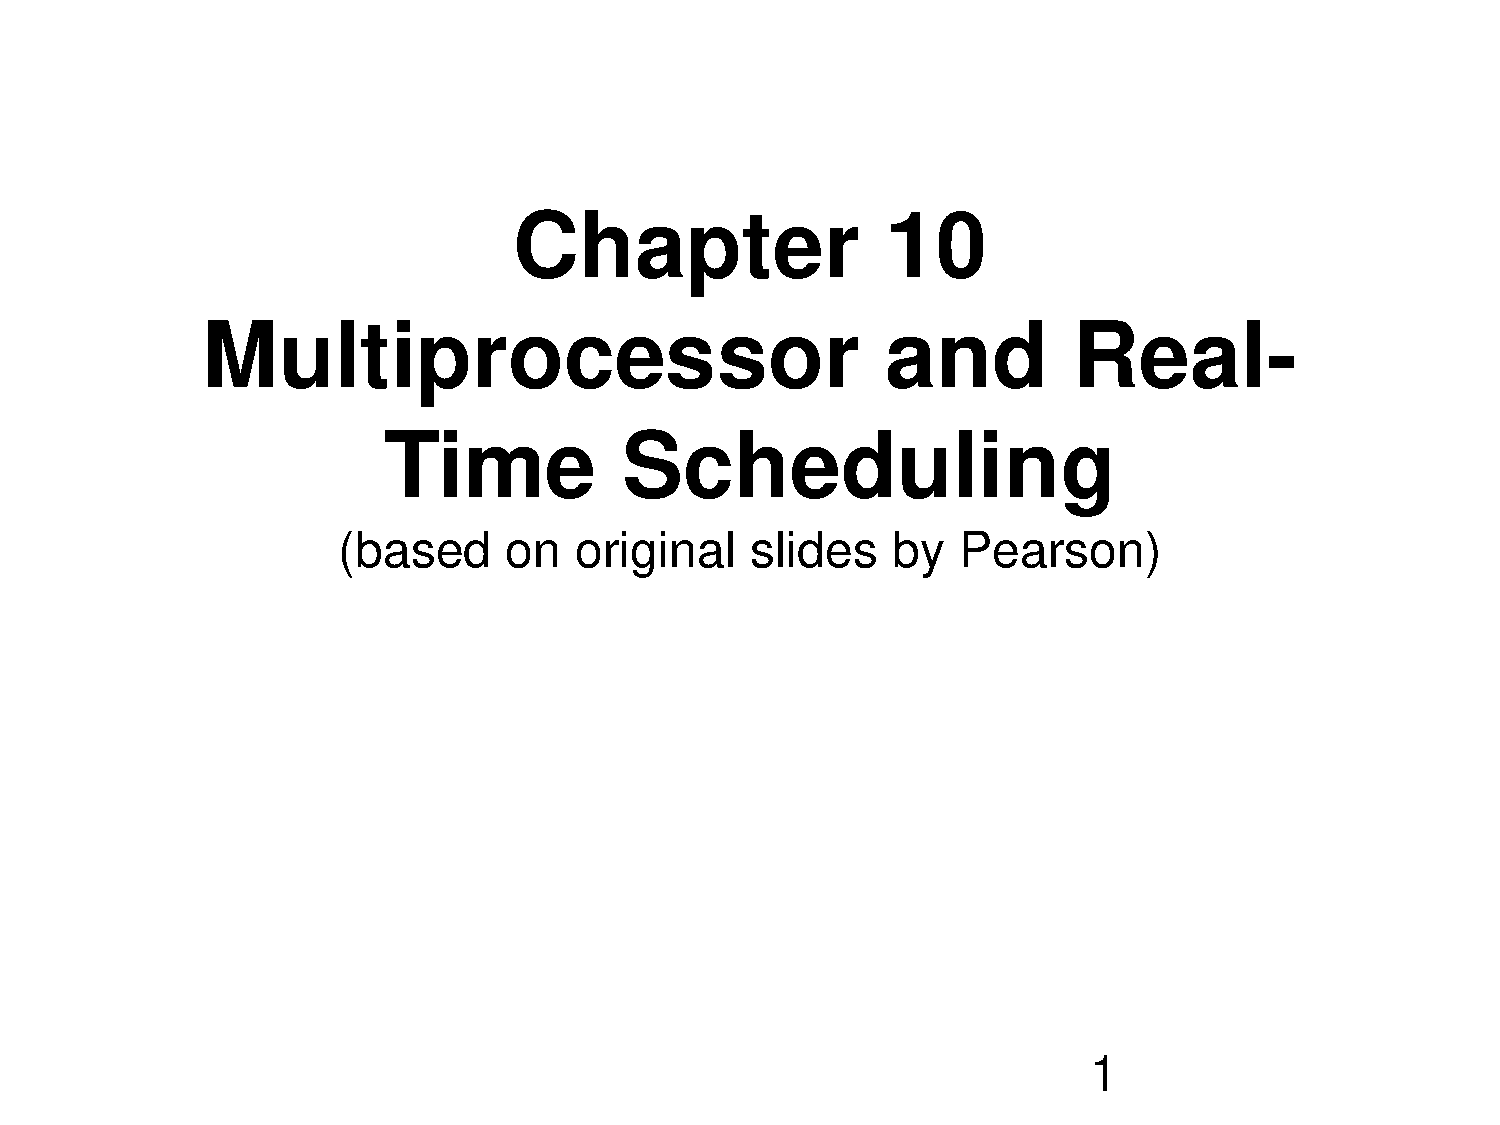
\includepdf[page=3]{10.pdf}
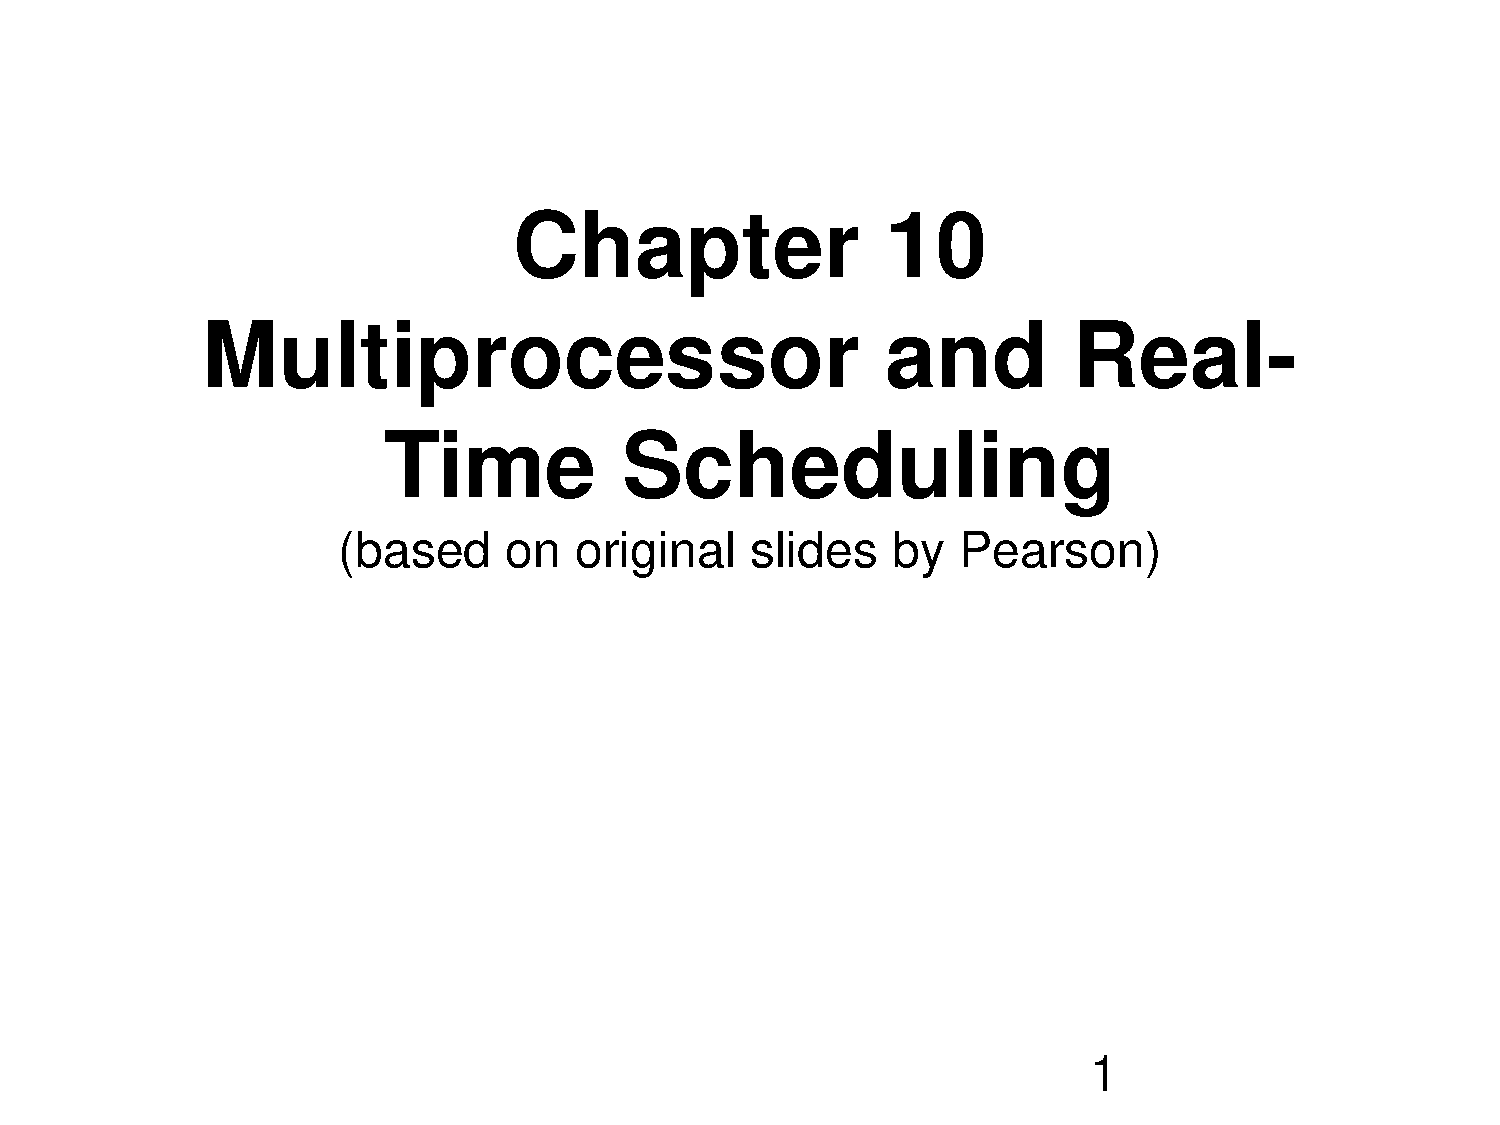
\includepdf[page=4]{10.pdf}
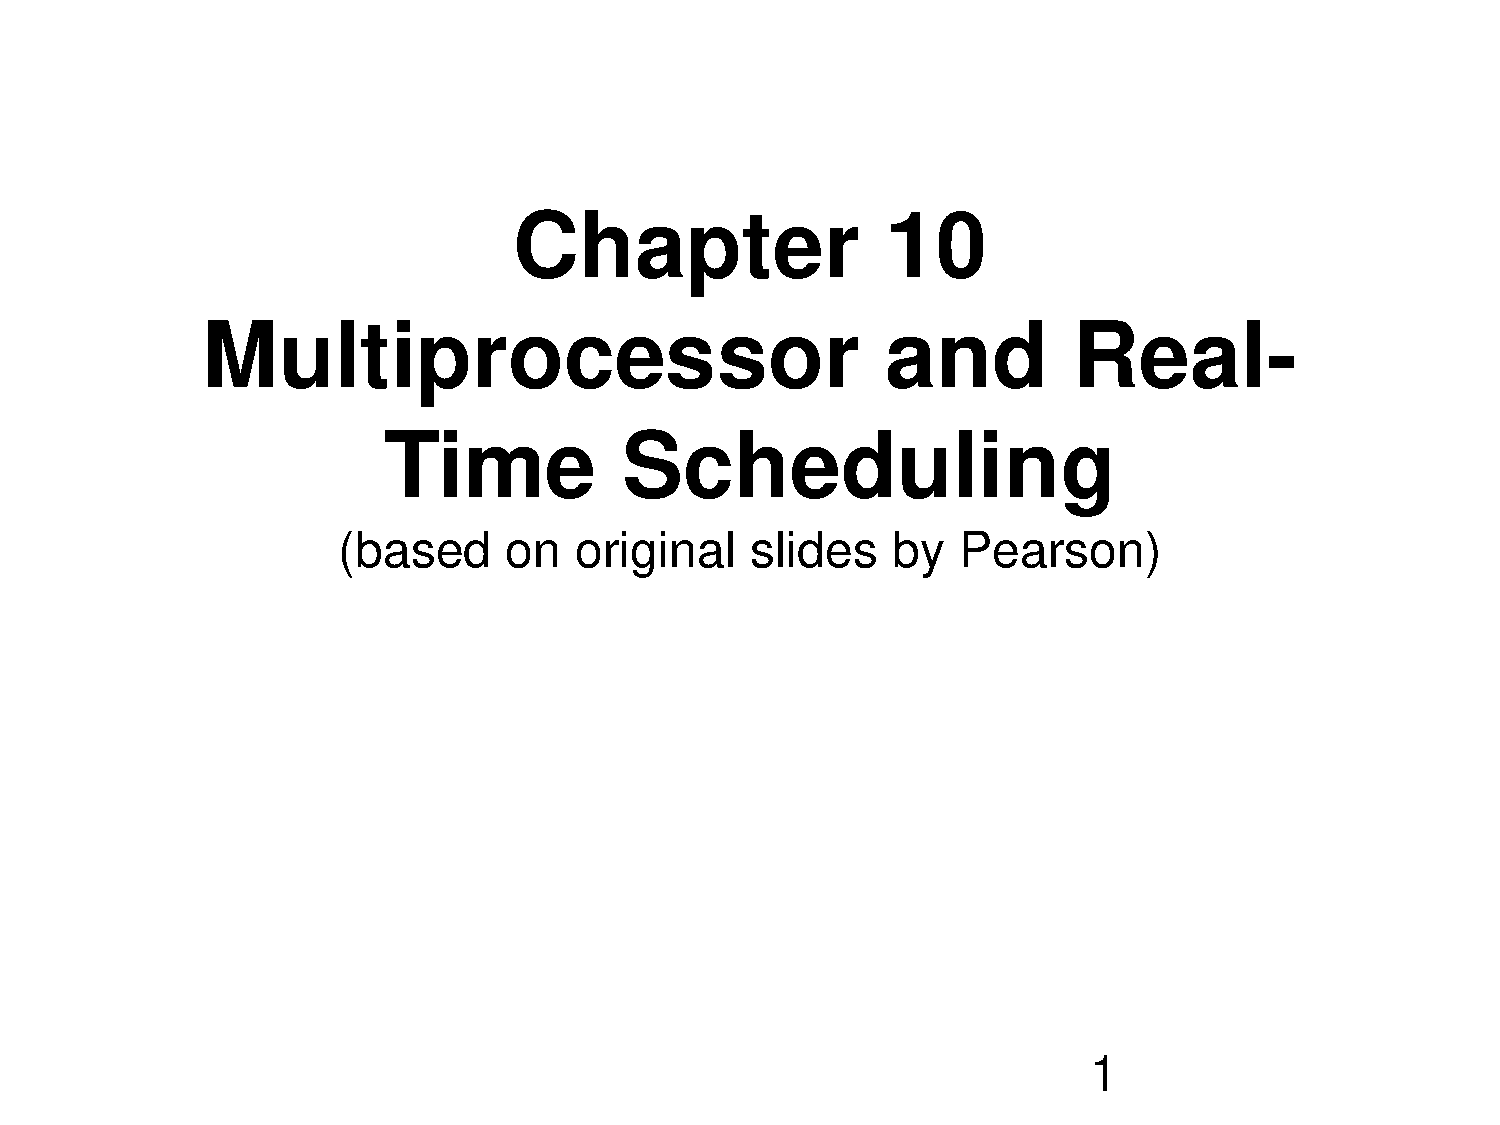
\includepdf[page=5]{10.pdf}
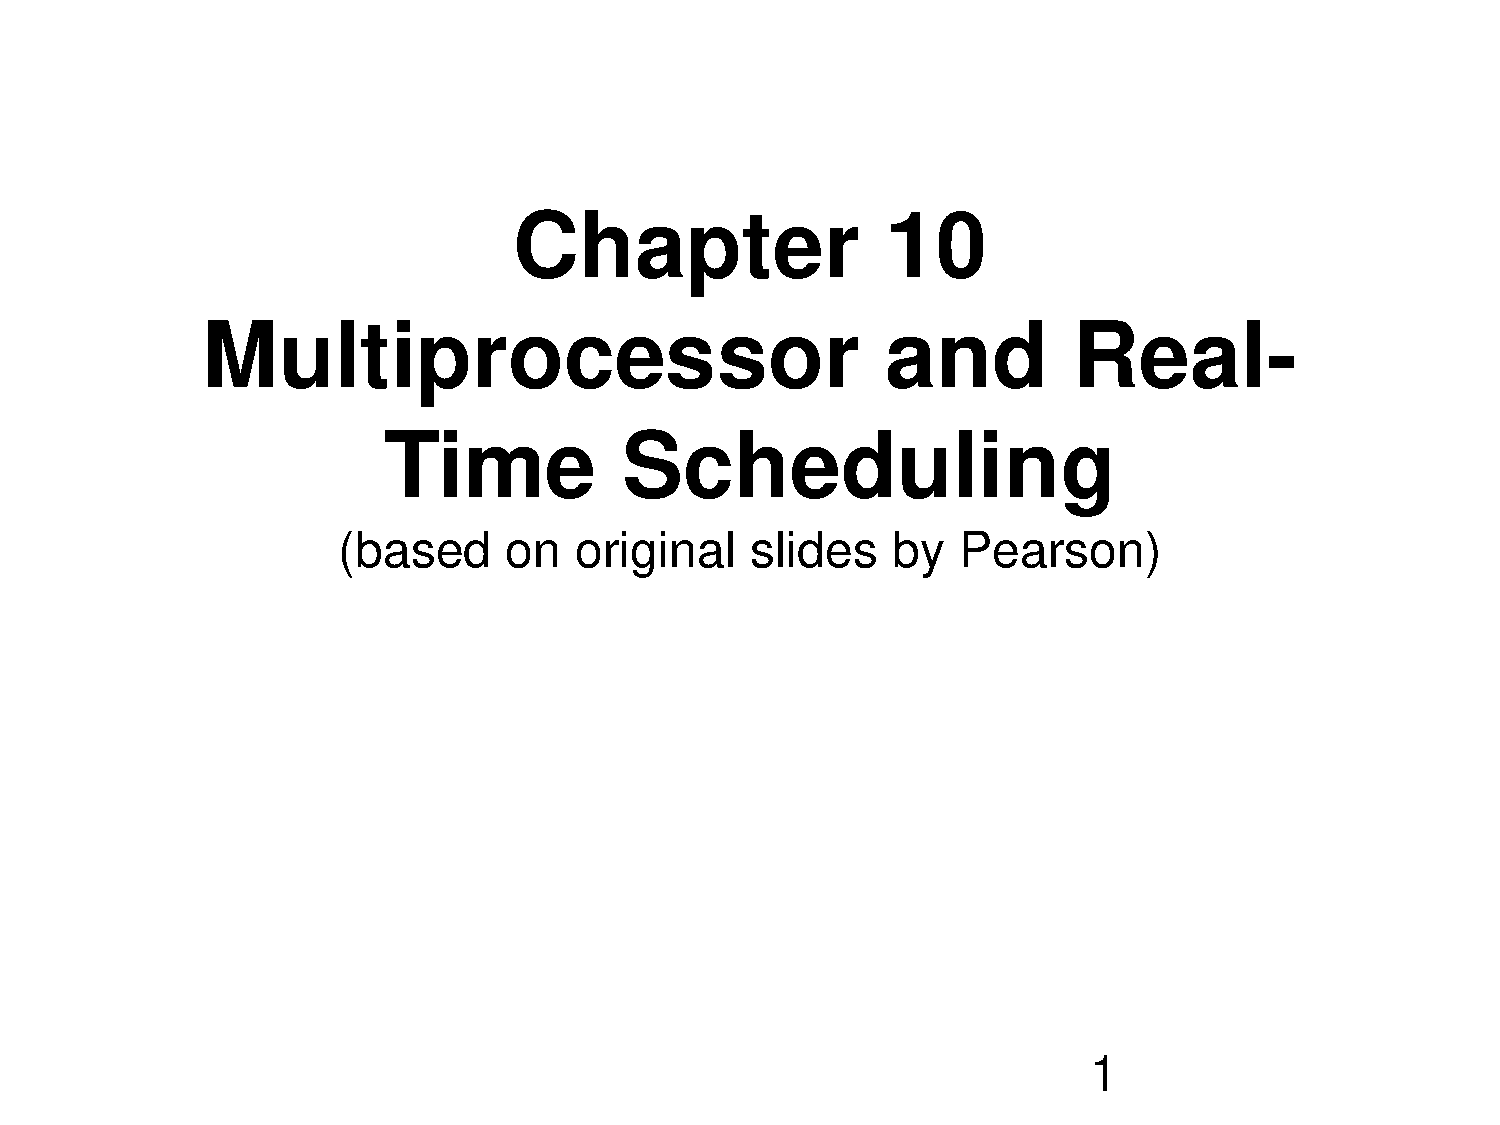
\includepdf[page=6]{10.pdf}
This is a classification of parallelism that is very similar to threading. In a multiprocessor system we can directly exploit threads.
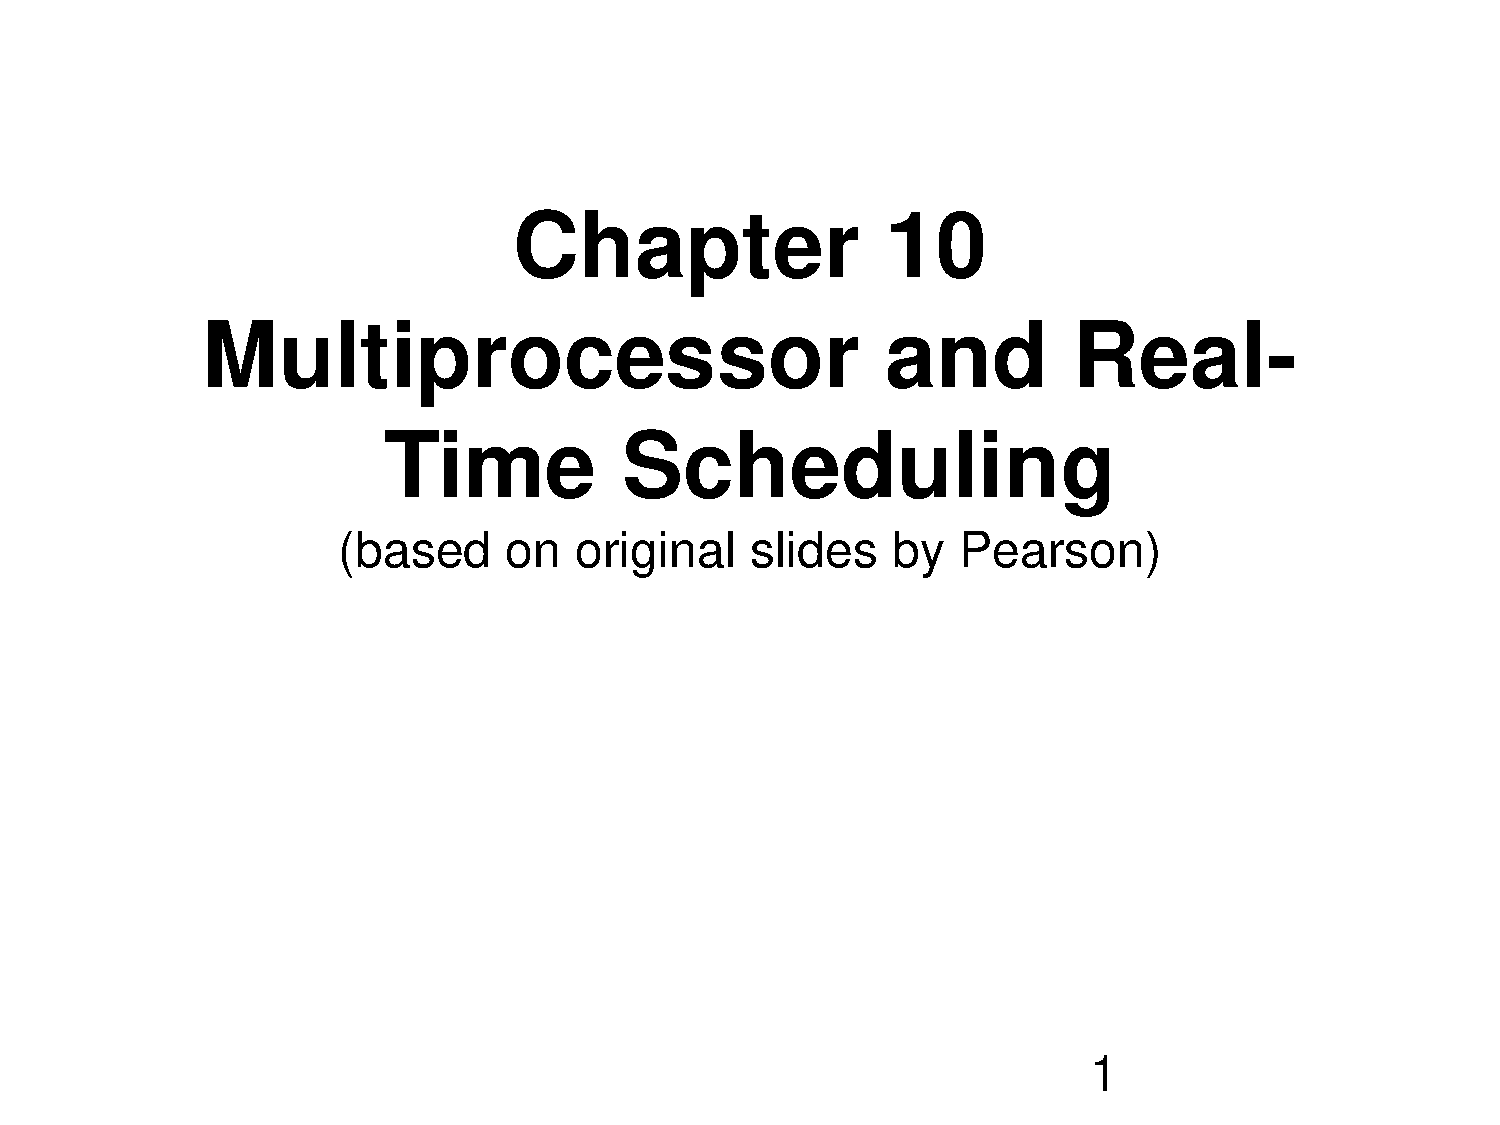
\includepdf[page=7]{10.pdf}
This is when we use multiprocessing to more quickly accomplish a single task (think high end computations).

Starting at fine graned parallelism and moving up:\\
SIMD is single instruction multiple data. We have multiple elements and one operation to apply to all elements at the same time.
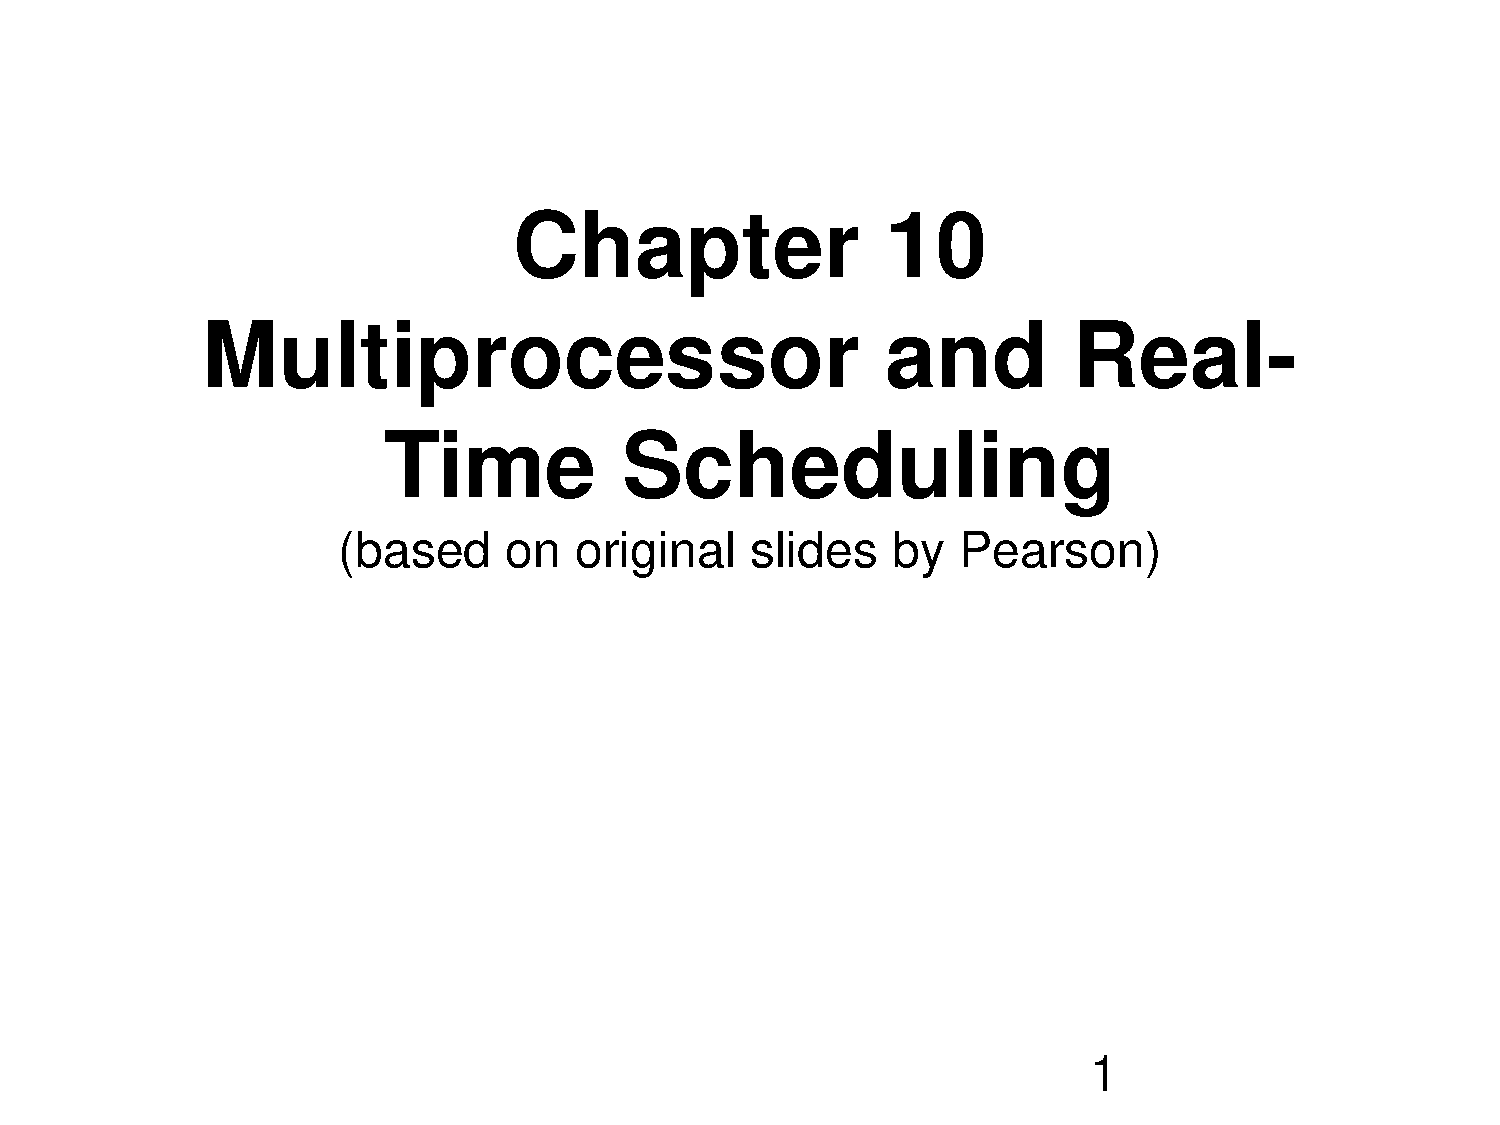
\includepdf[page=8]{10.pdf}
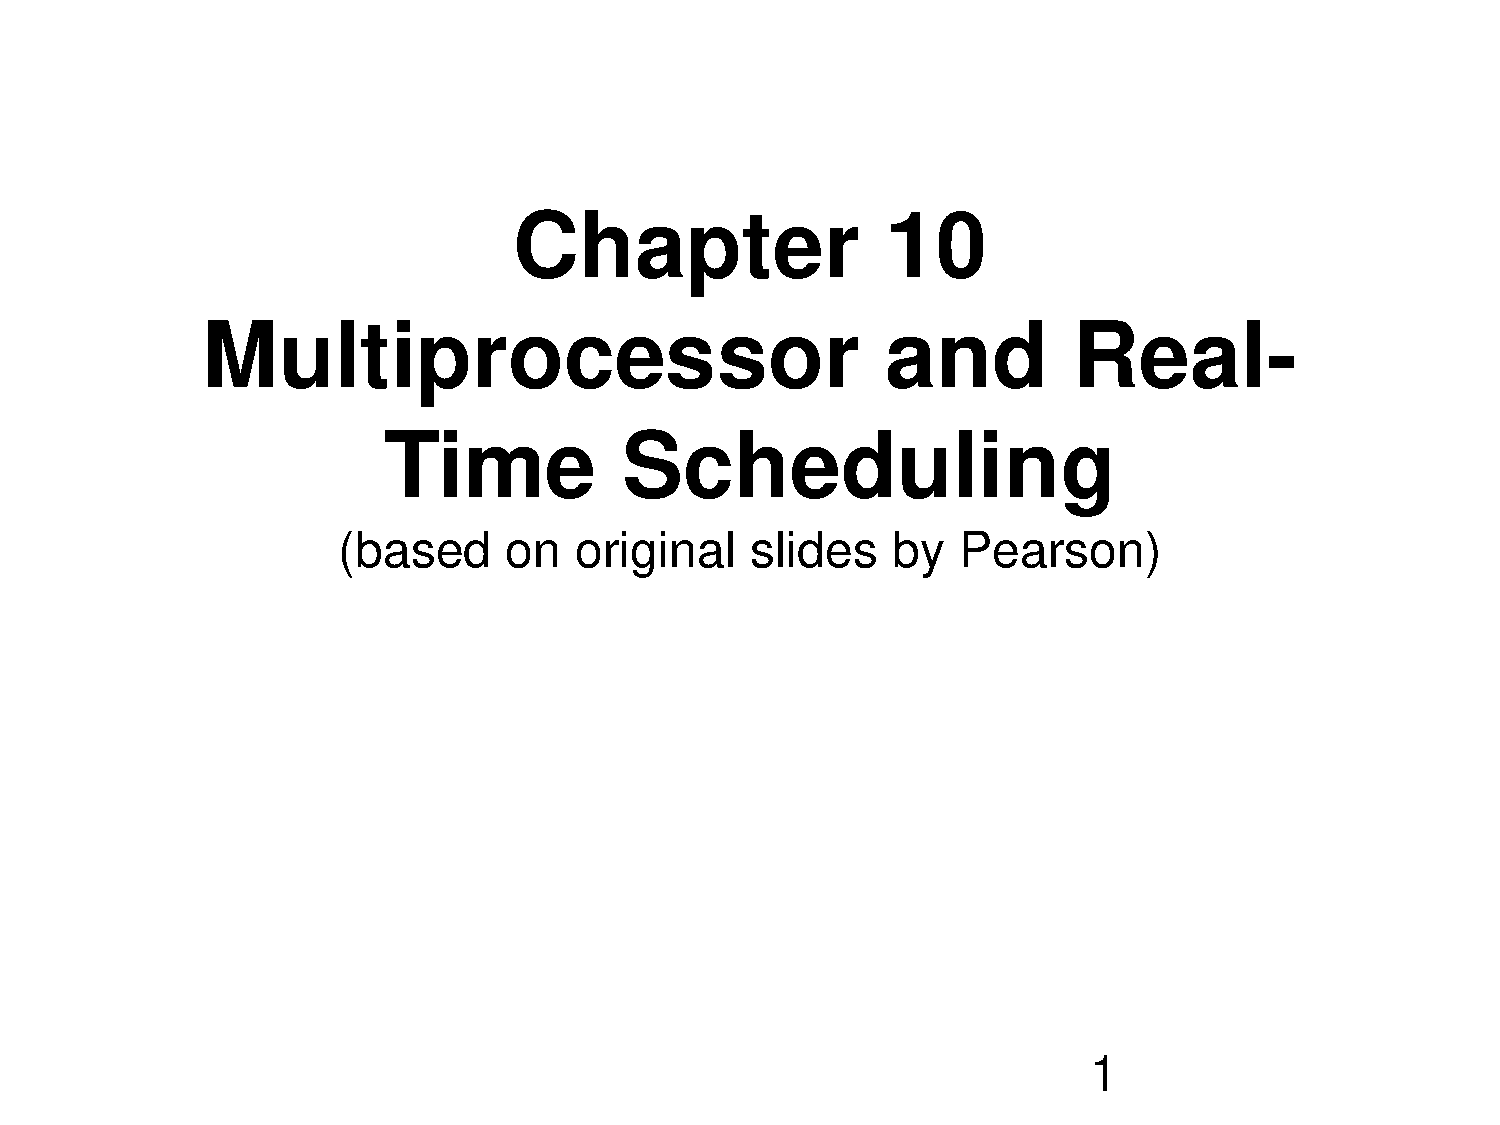
\includepdf[page=9]{10.pdf}
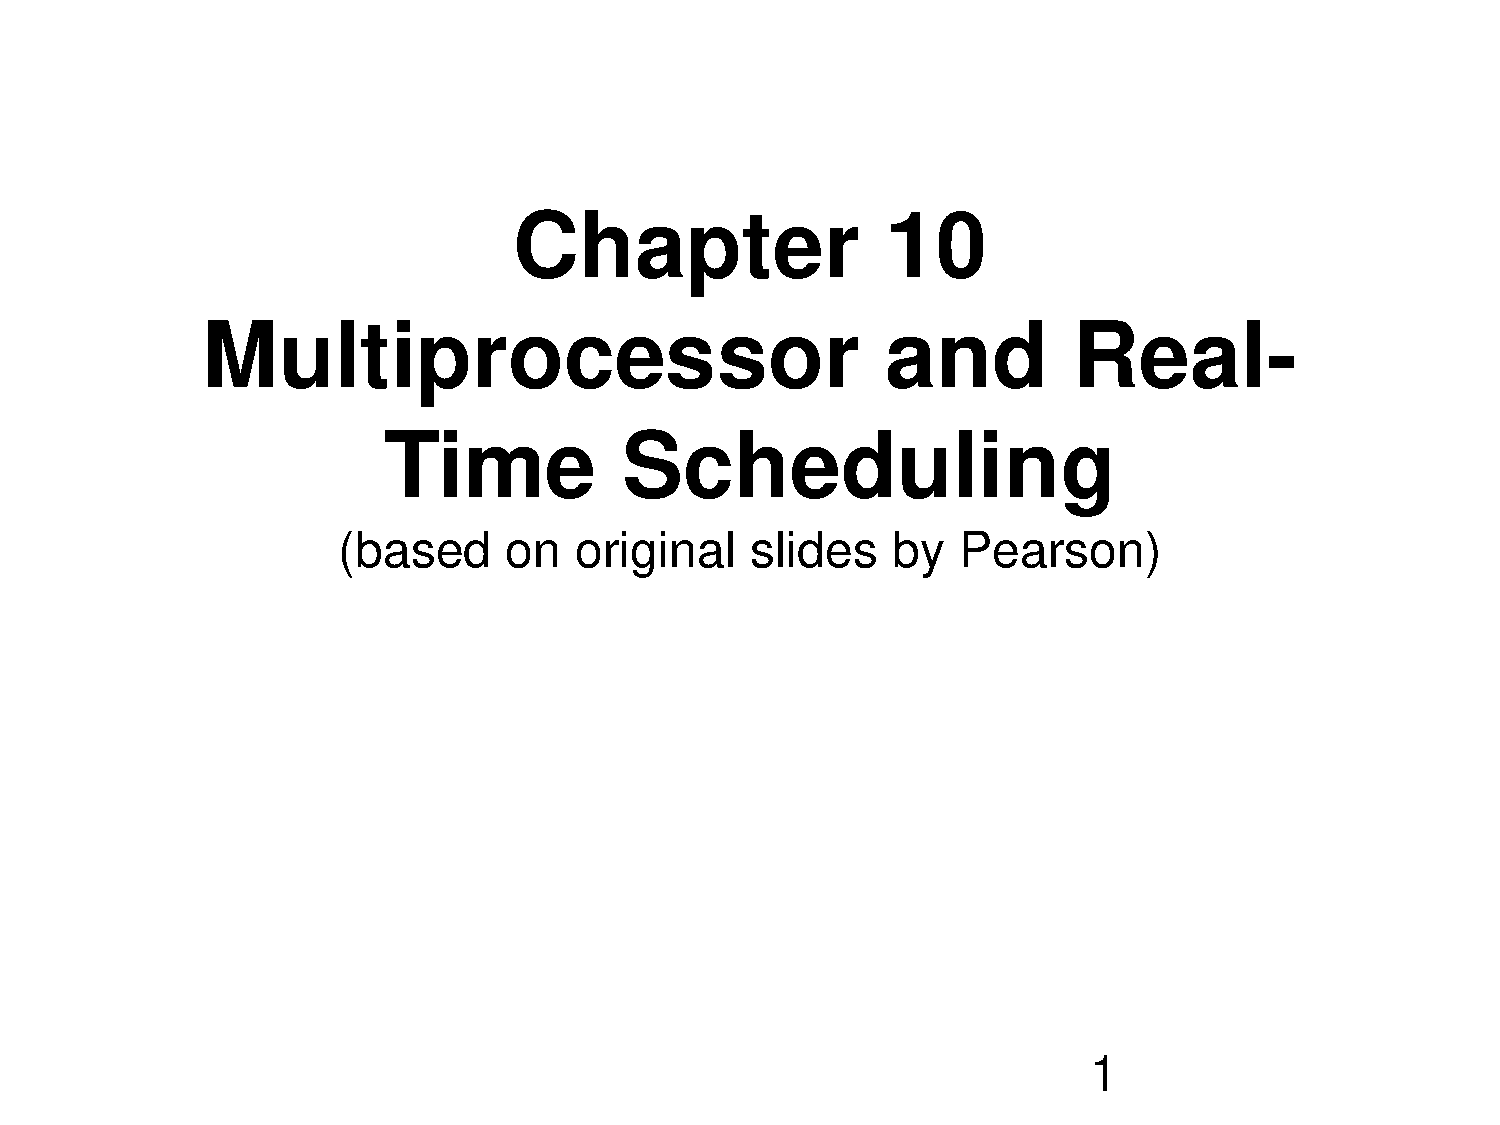
\includepdf[page=10]{10.pdf}
The fuck is he talking about

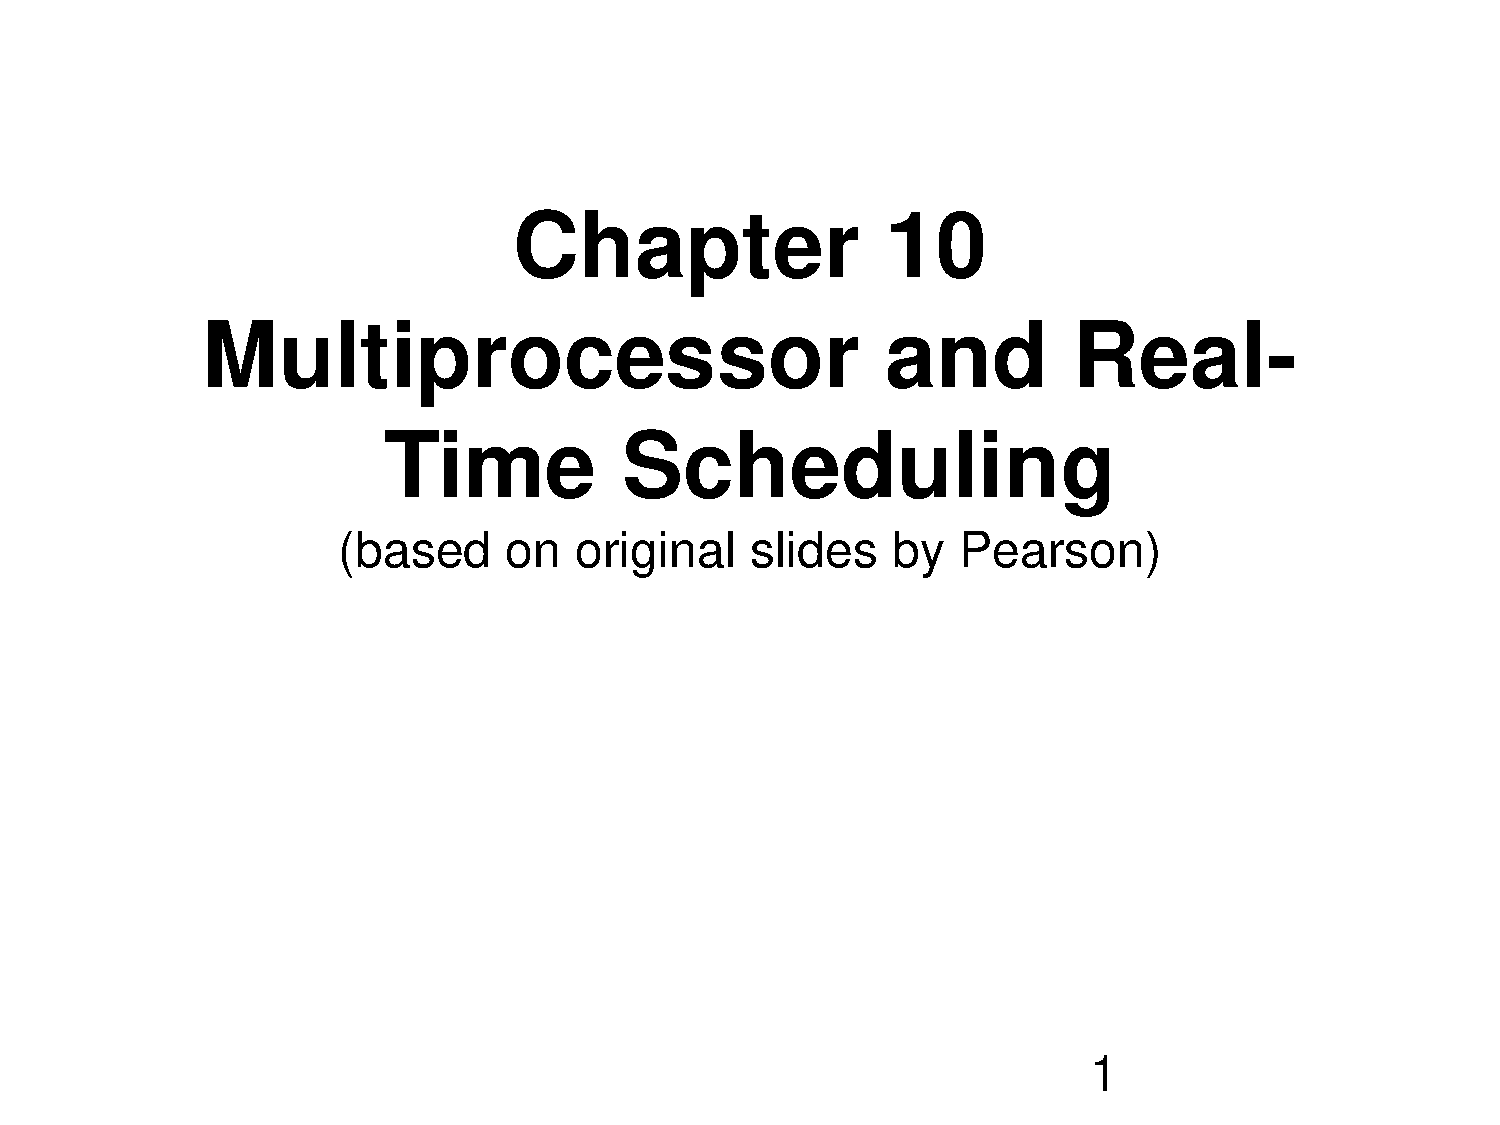
\includepdf[page=11]{10.pdf}
Static assignment allows batching but some processes will be idle.

Process migration can have high overhead when migrating the  process between cores.

Hybrid uses a separate cache on each core, but shared memory between them. Here virtual memory calculations are done on the cache level.
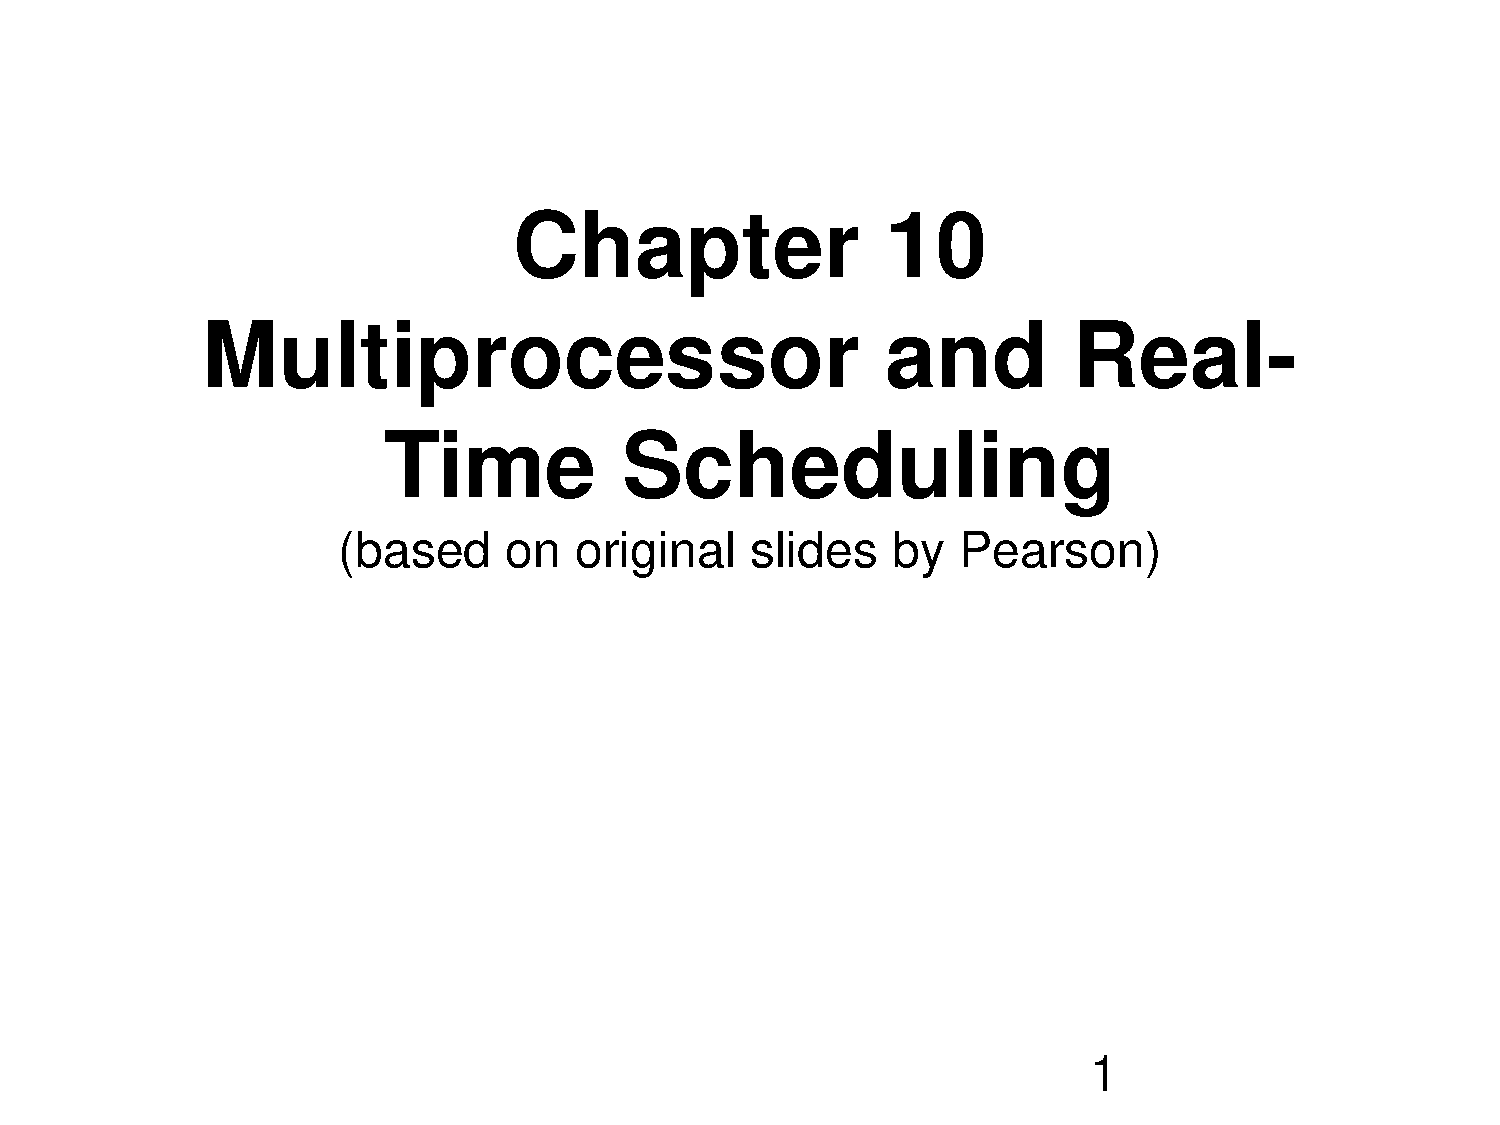
\includepdf[page=12]{10.pdf}
Where do we run the OS? We often have the kernel run on a particular processor that does all of the scheduling and housekeeping called the master processor. All other processes send their requests through the master core. The downside of this is that if the master core gets buggered in anyway we take down everything. We also dont have the OS using multiprocessing.
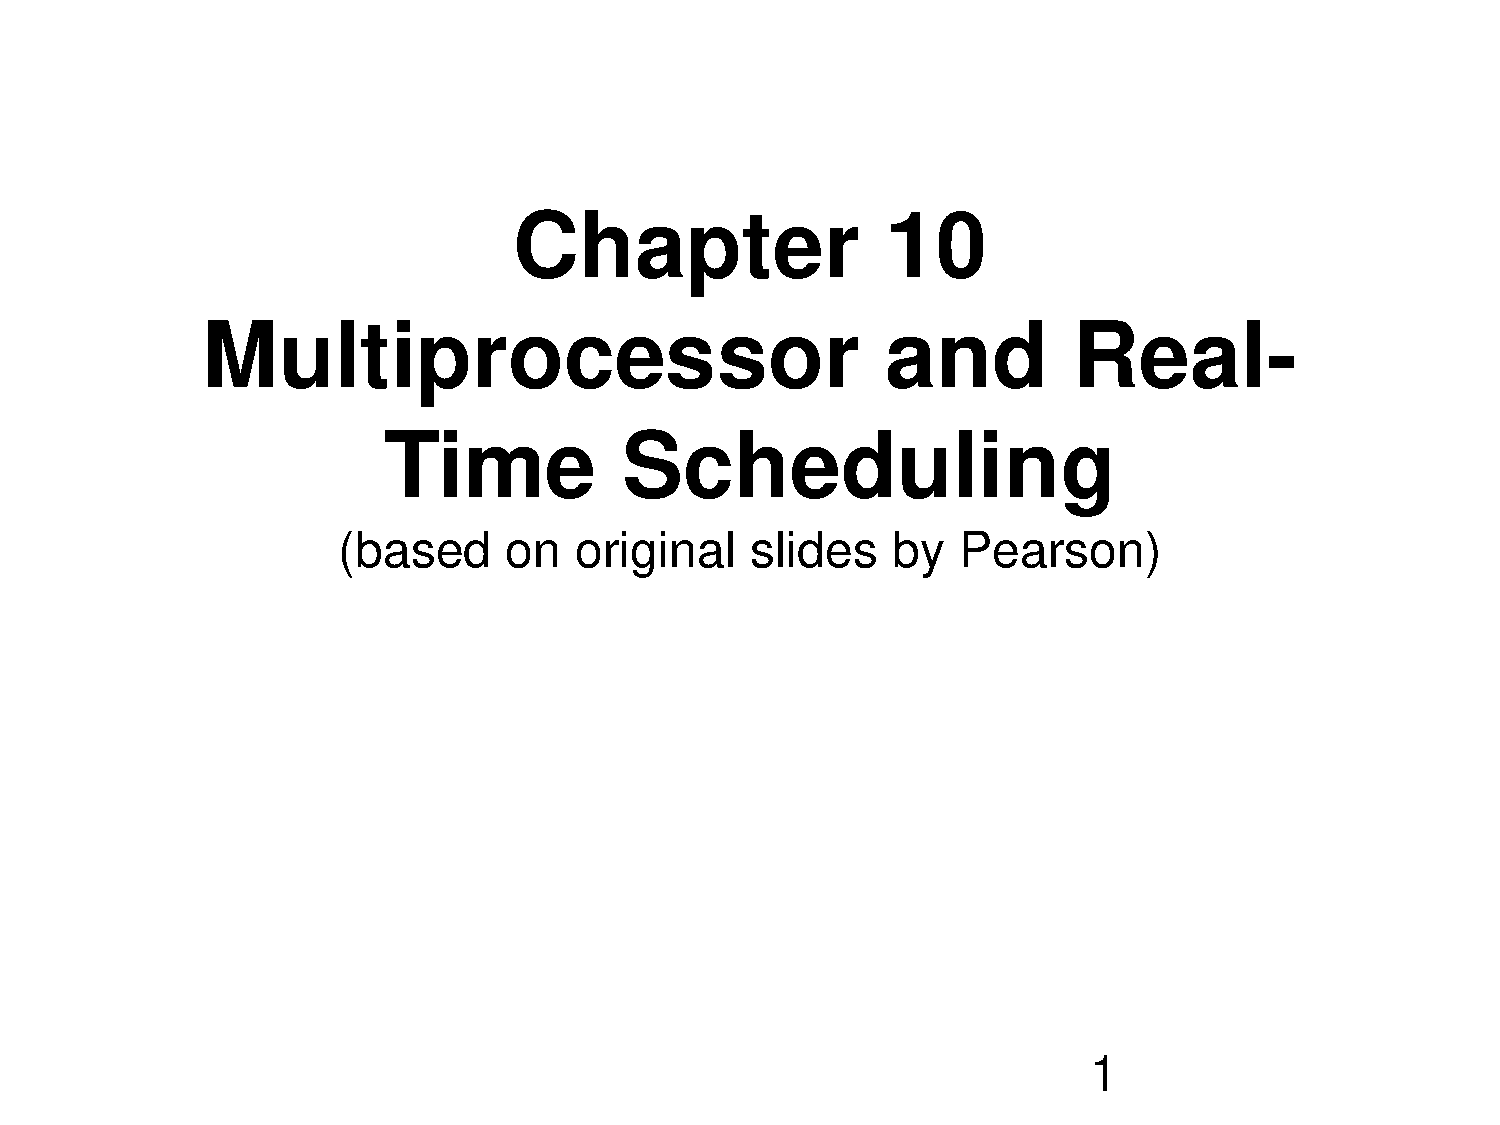
\includepdf[page=13]{10.pdf}
Here the kernel can execute on any processor. but the processor does its own scheduling. Downside is that all of the shared resources still have to be managed so things get much more complicated.
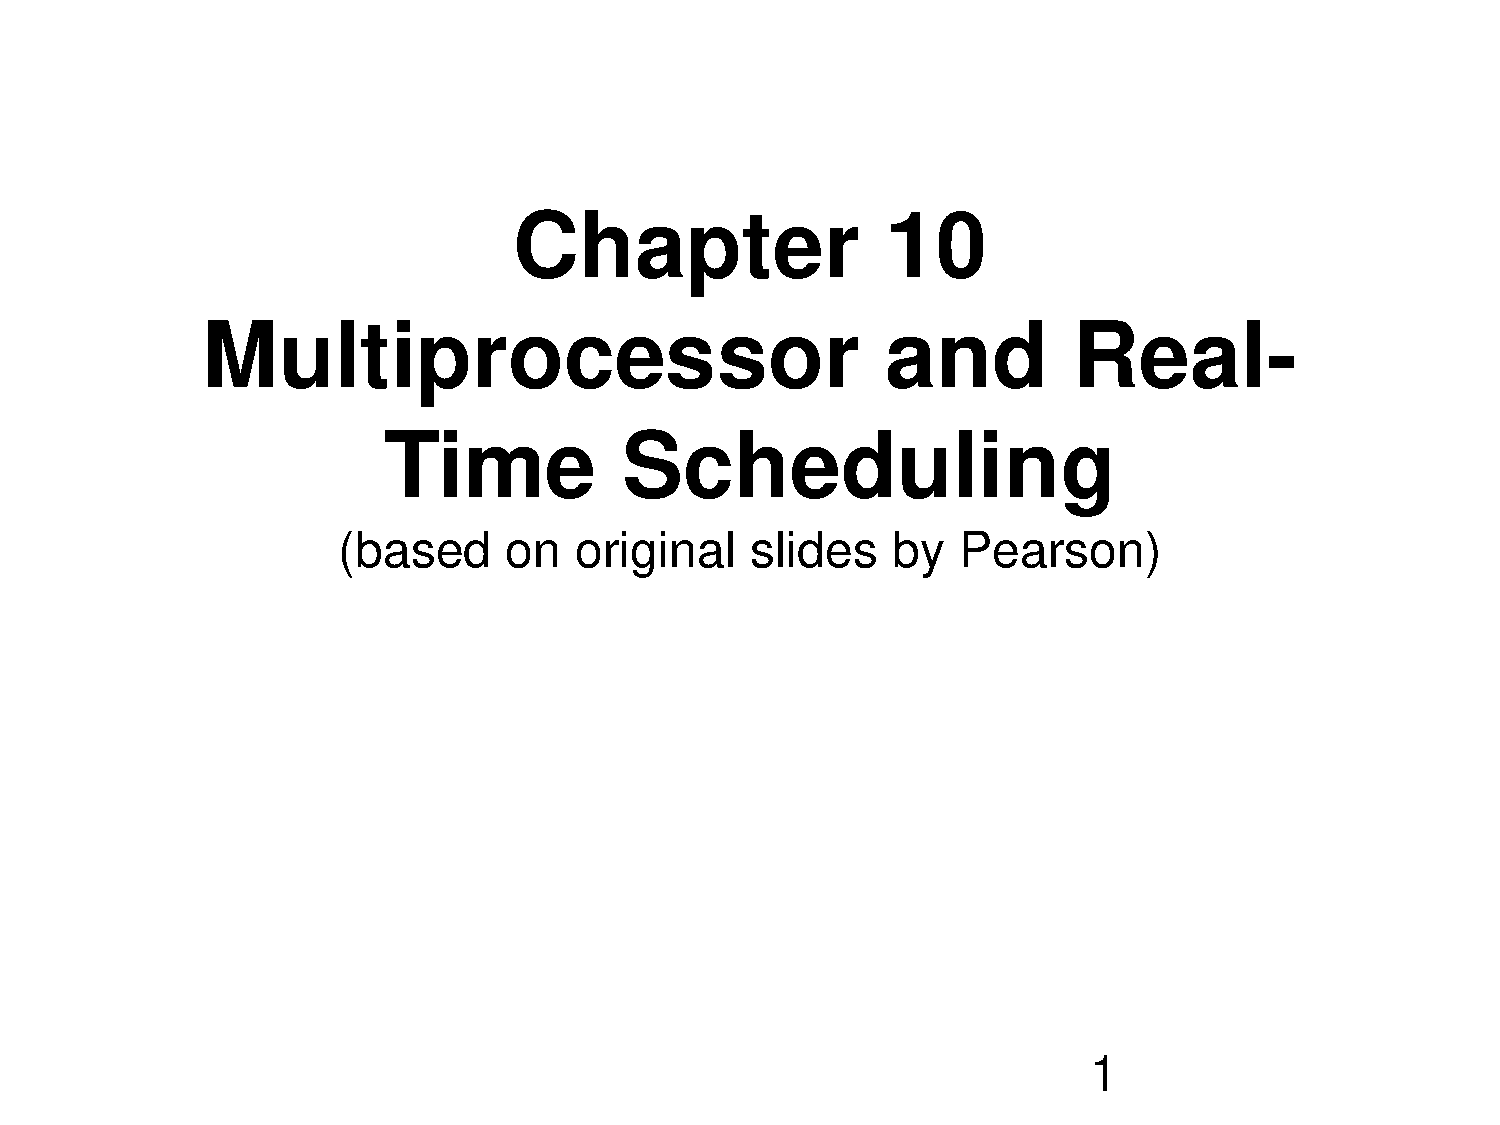
\includepdf[page=14]{10.pdf}
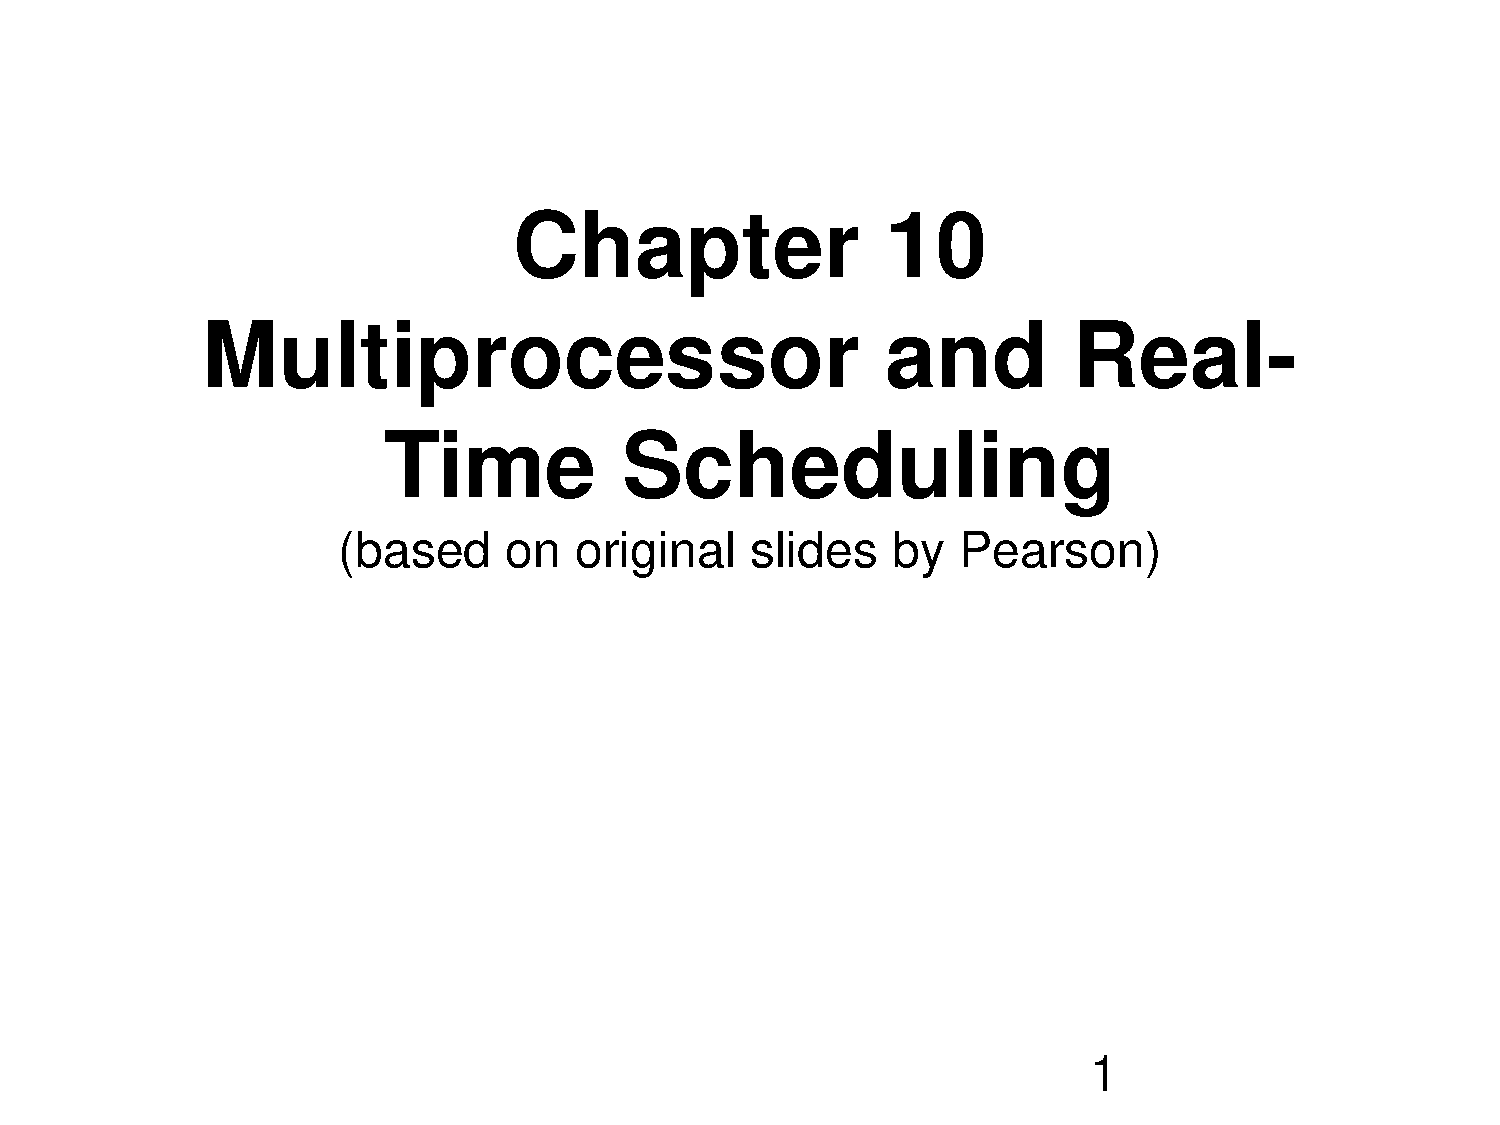
\includepdf[page=15]{10.pdf}
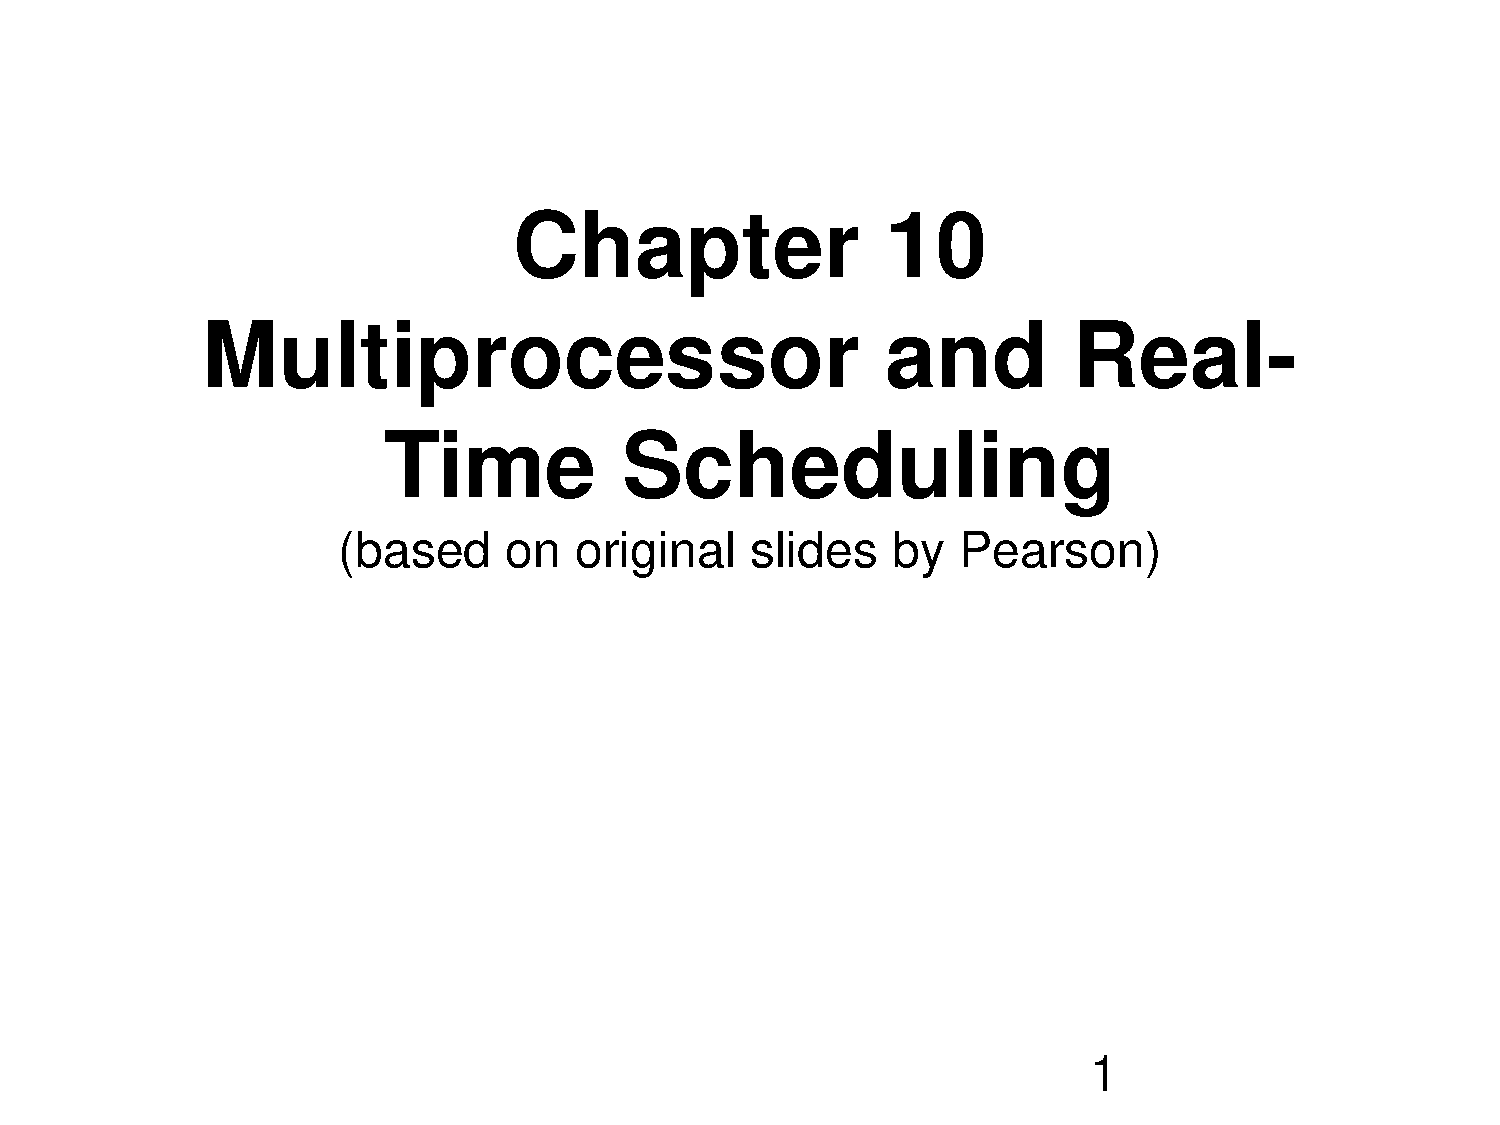
\includepdf[page=16]{10.pdf}
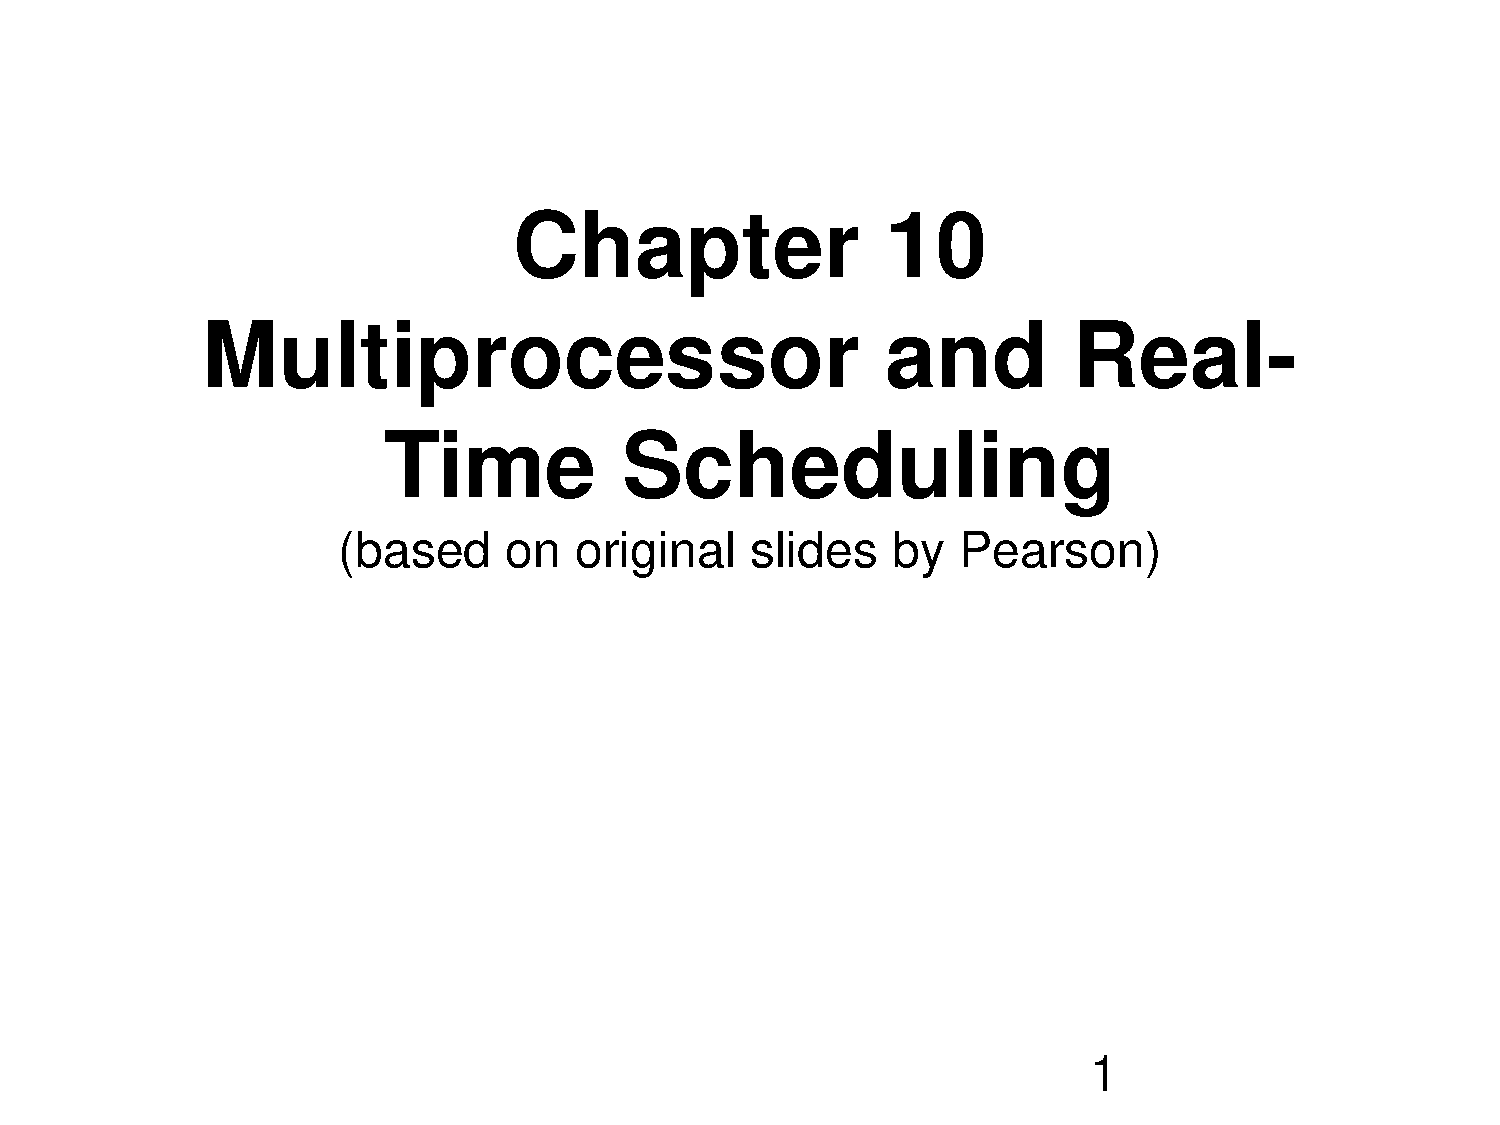
\includepdf[page=17]{10.pdf}
This graph shows how the theoughput of round robin scheduling is effected by the coefficient of variation (still dont know what that is)
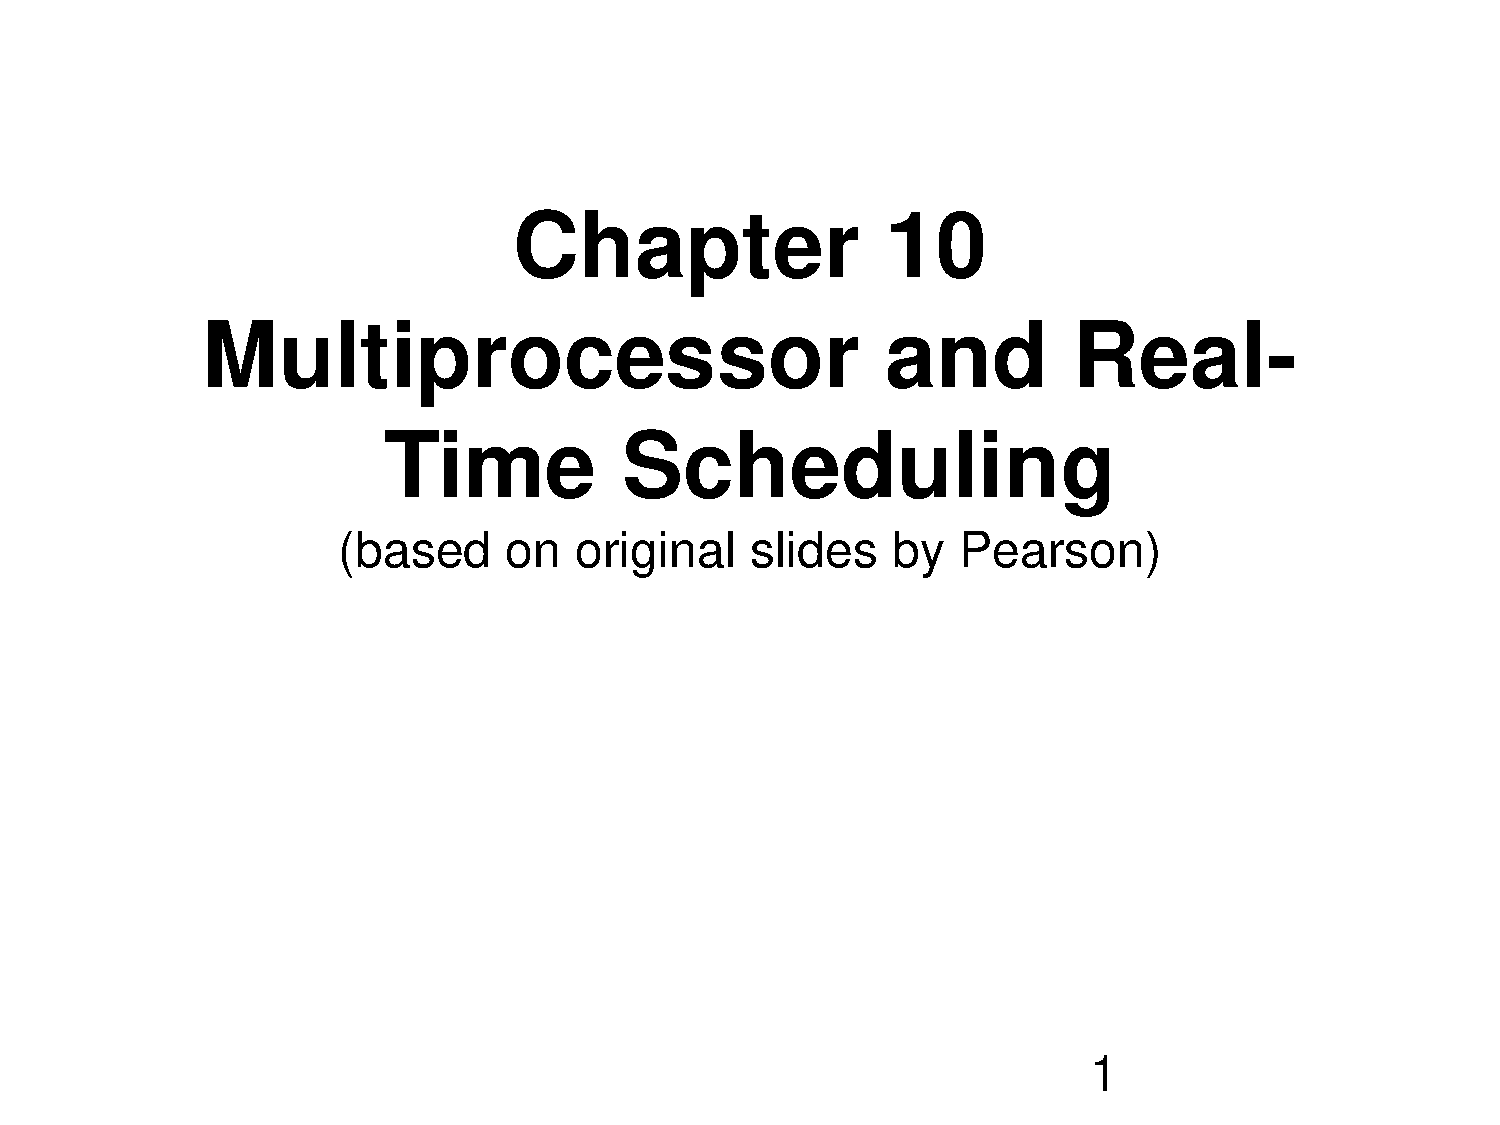
\includepdf[page=18]{10.pdf}
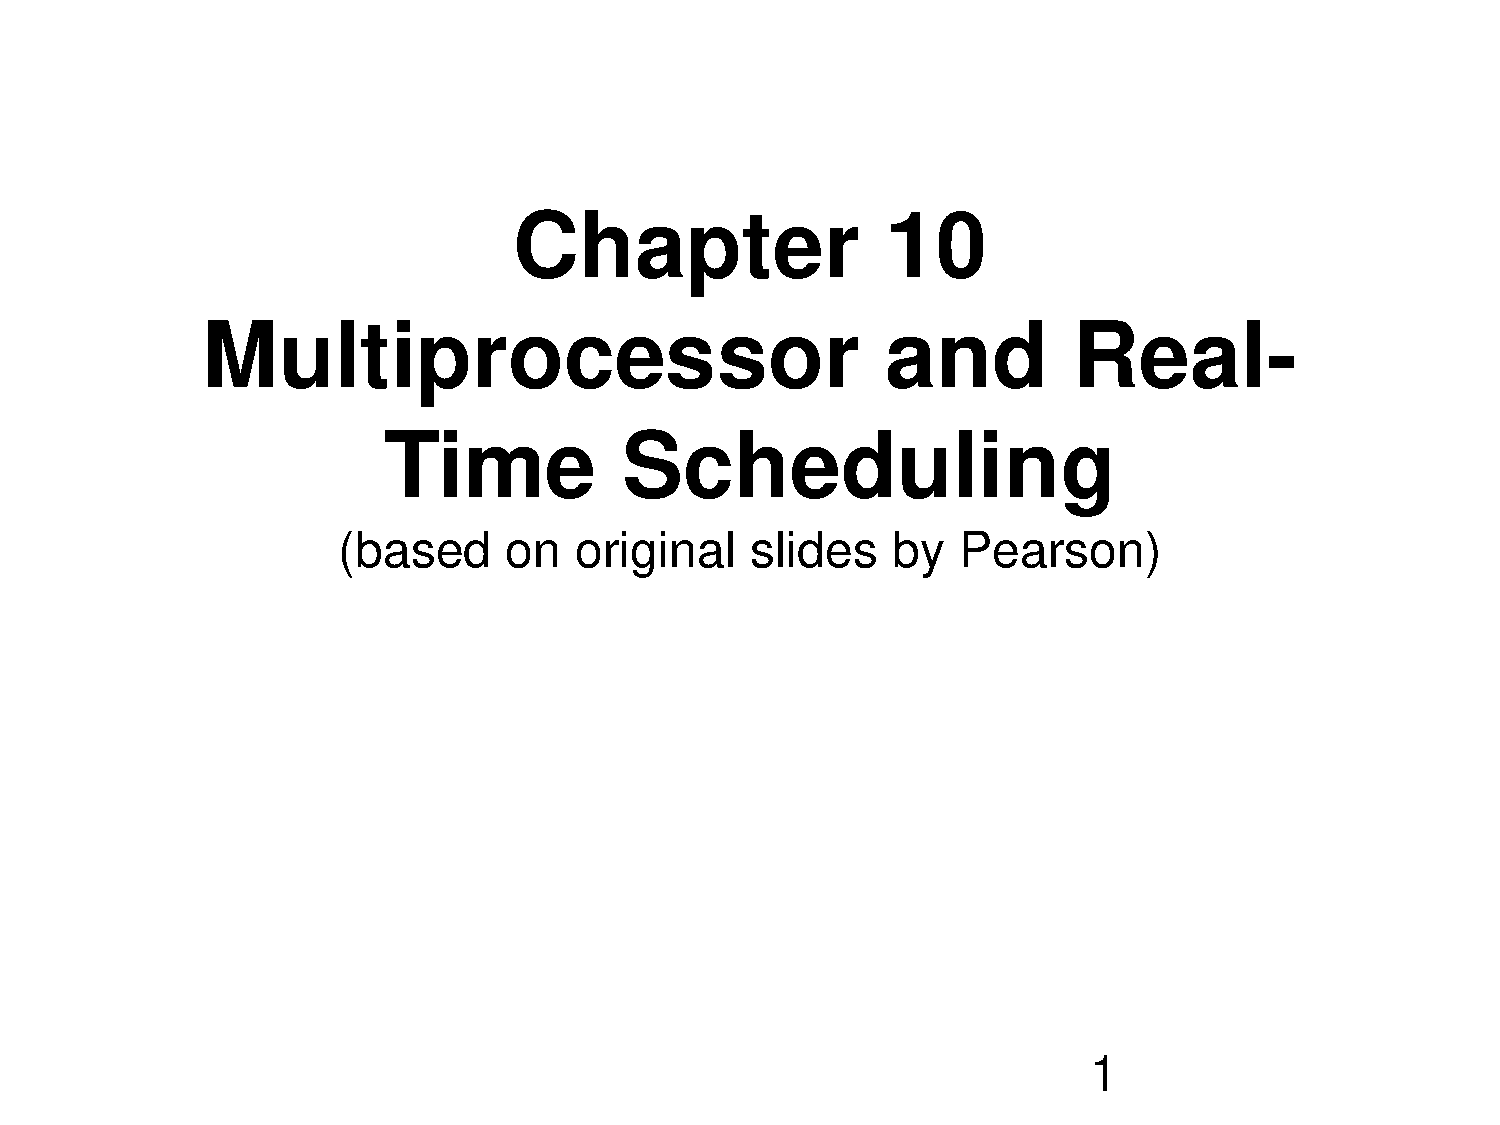
\includepdf[page=19]{10.pdf}
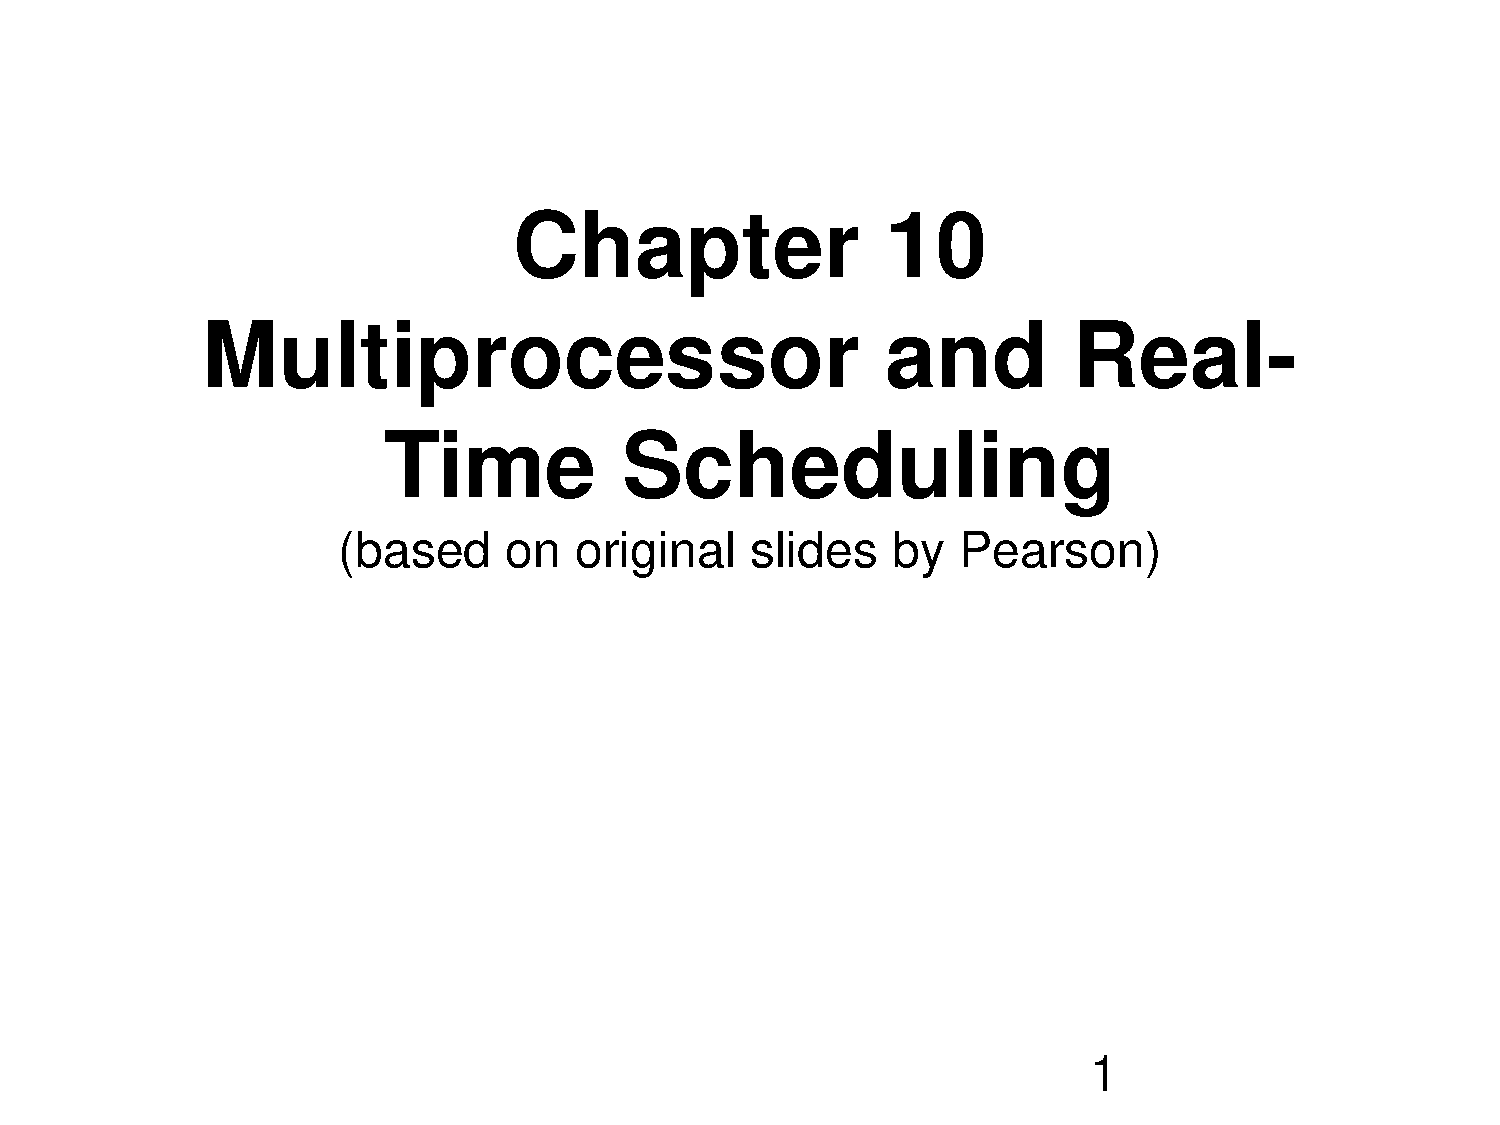
\includepdf[page=20]{10.pdf}
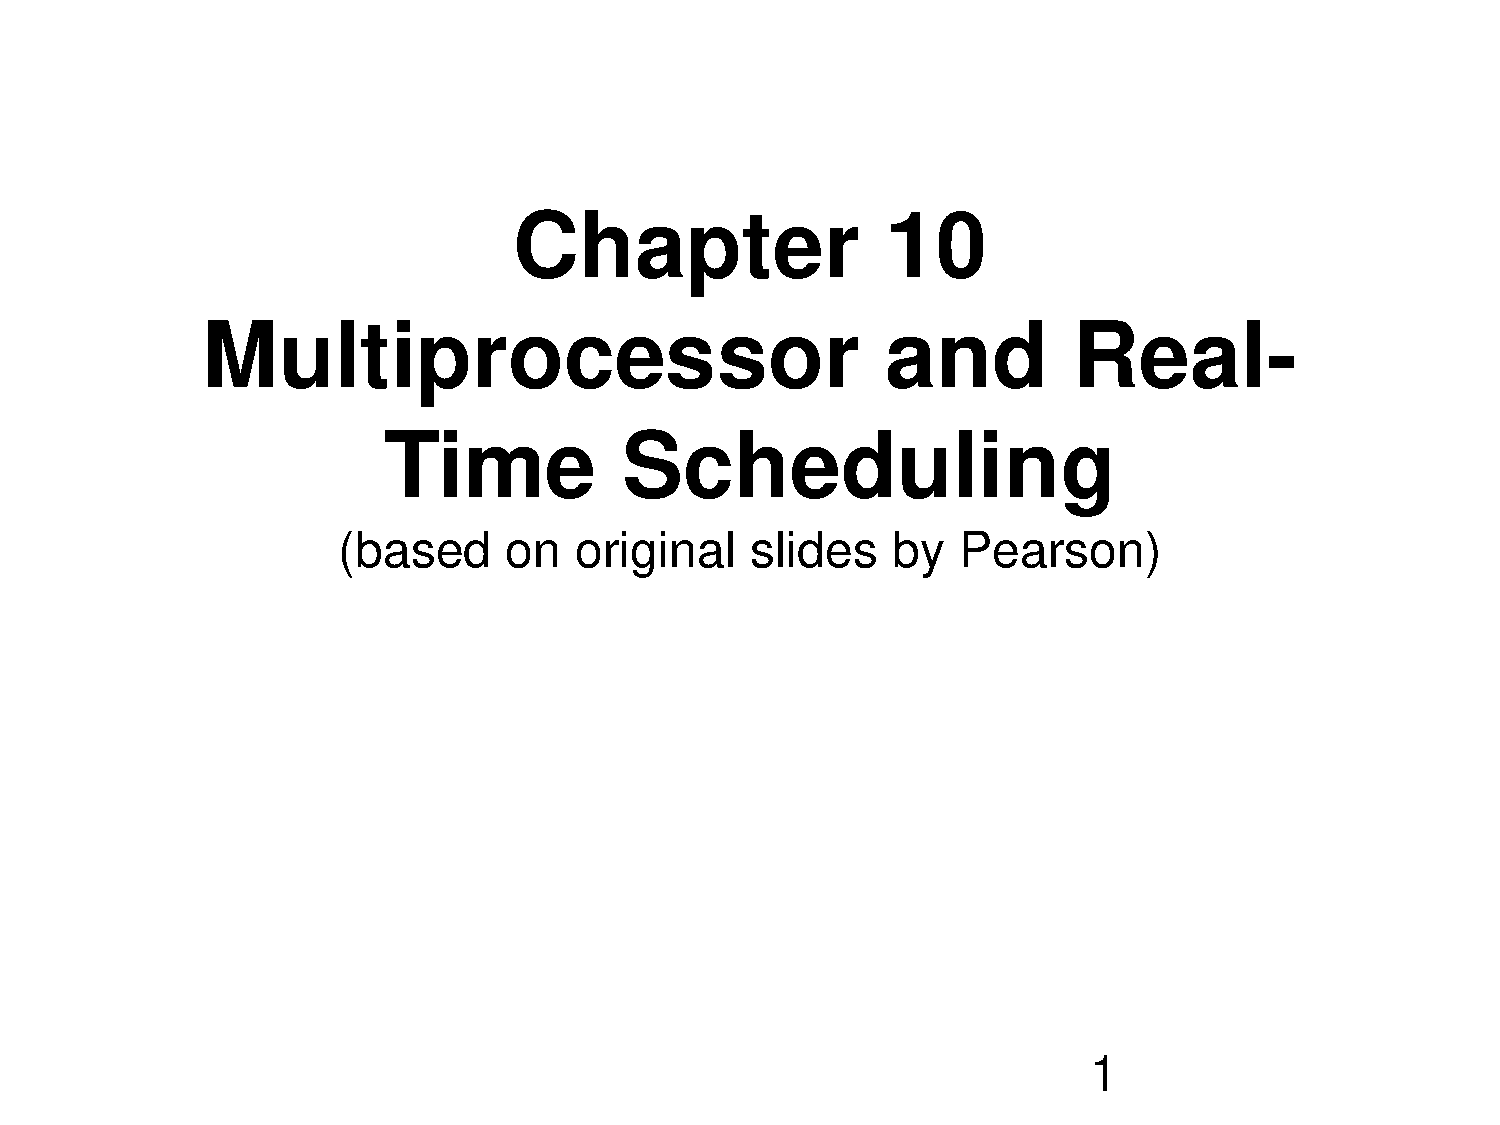
\includepdf[page=21]{10.pdf}
When a thread is stopped and started it probably wont be on the same processor so memory management is started over again which sucks.

We have no control over the order of execution.
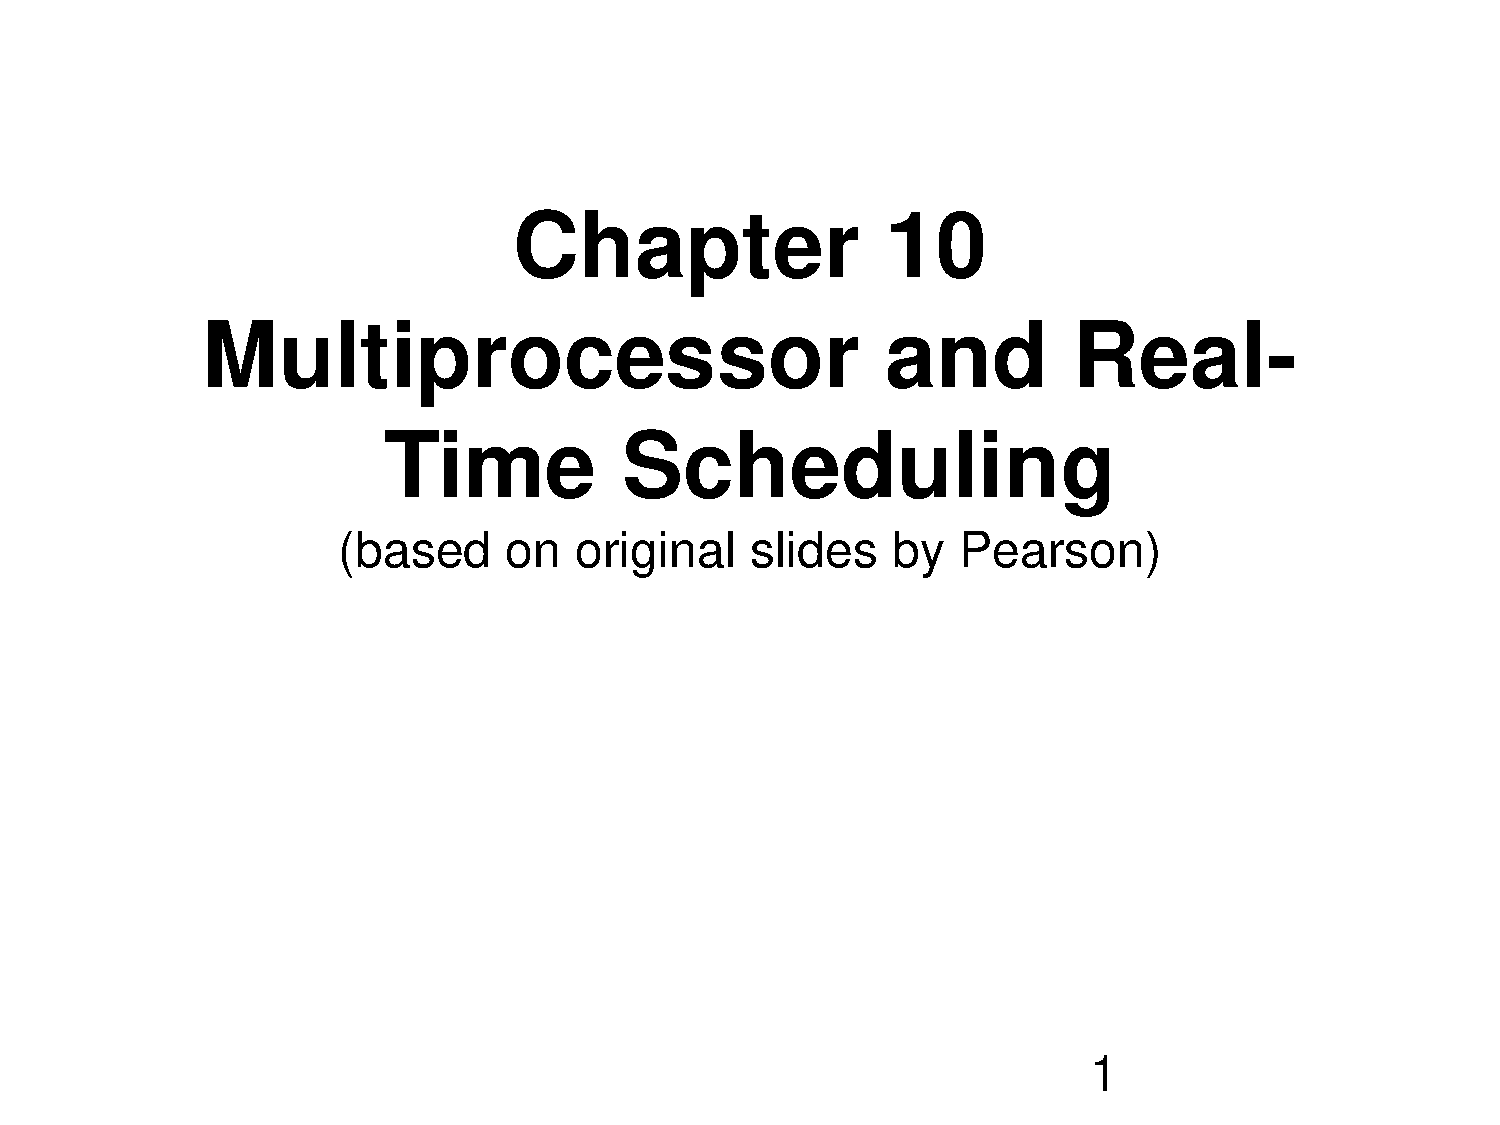
\includepdf[page=22]{10.pdf}
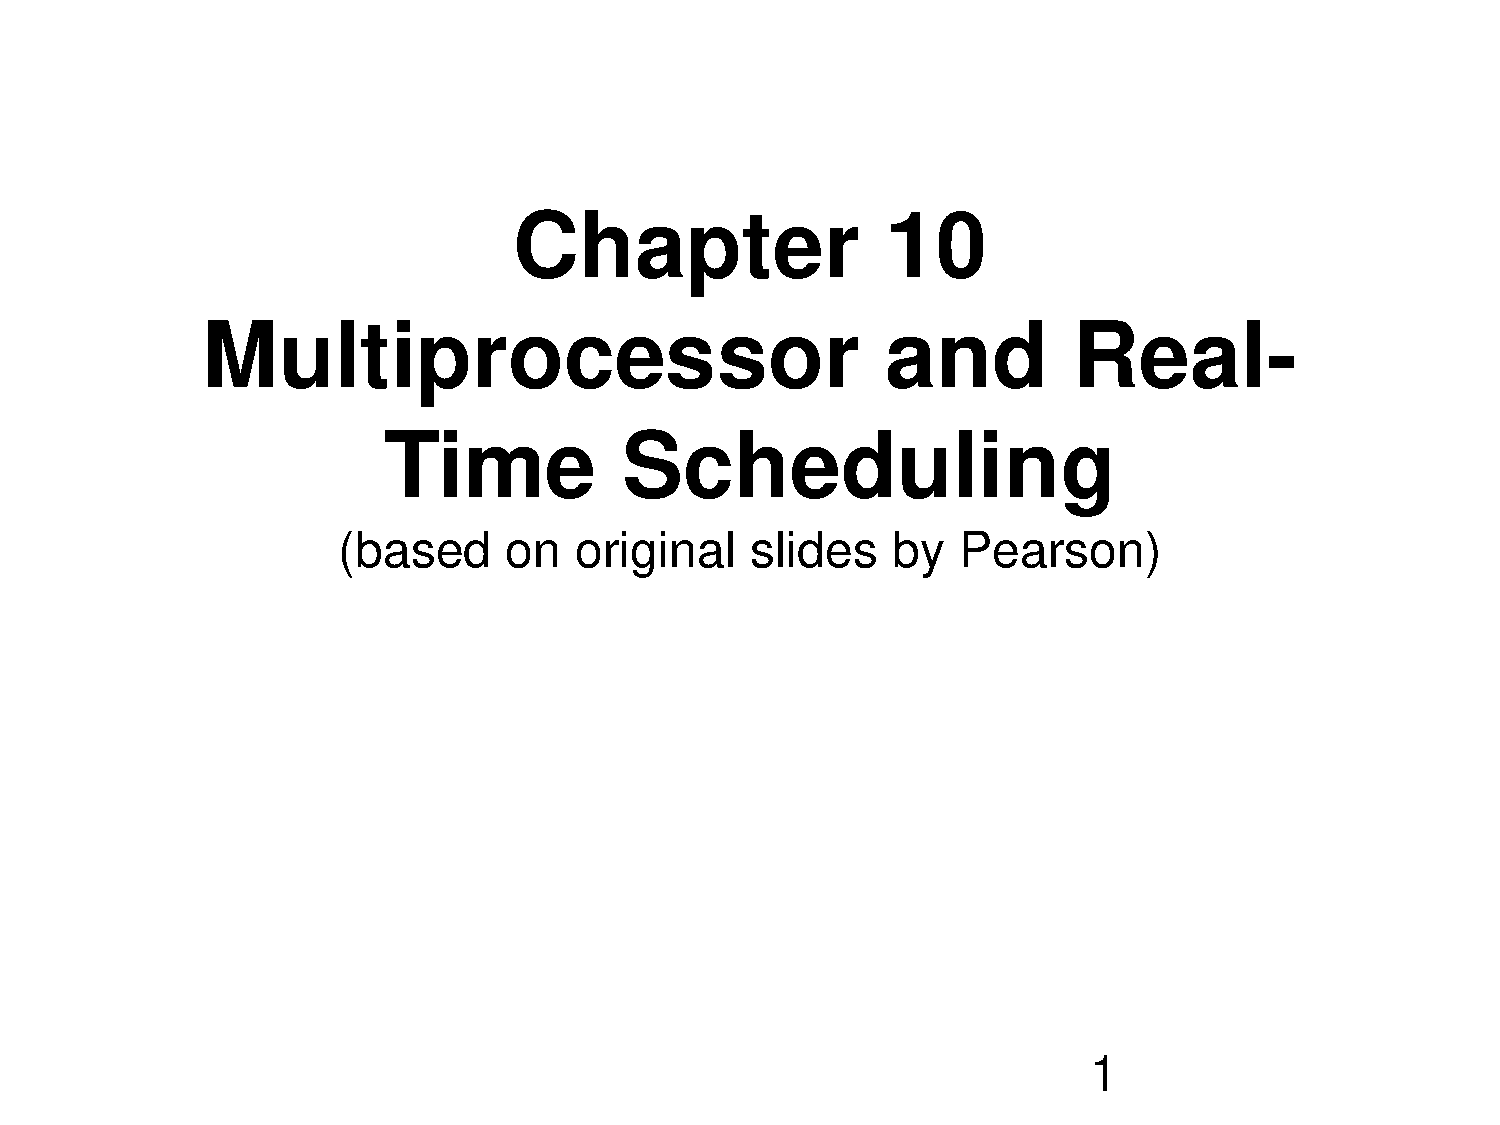
\includepdf[page=23]{10.pdf}
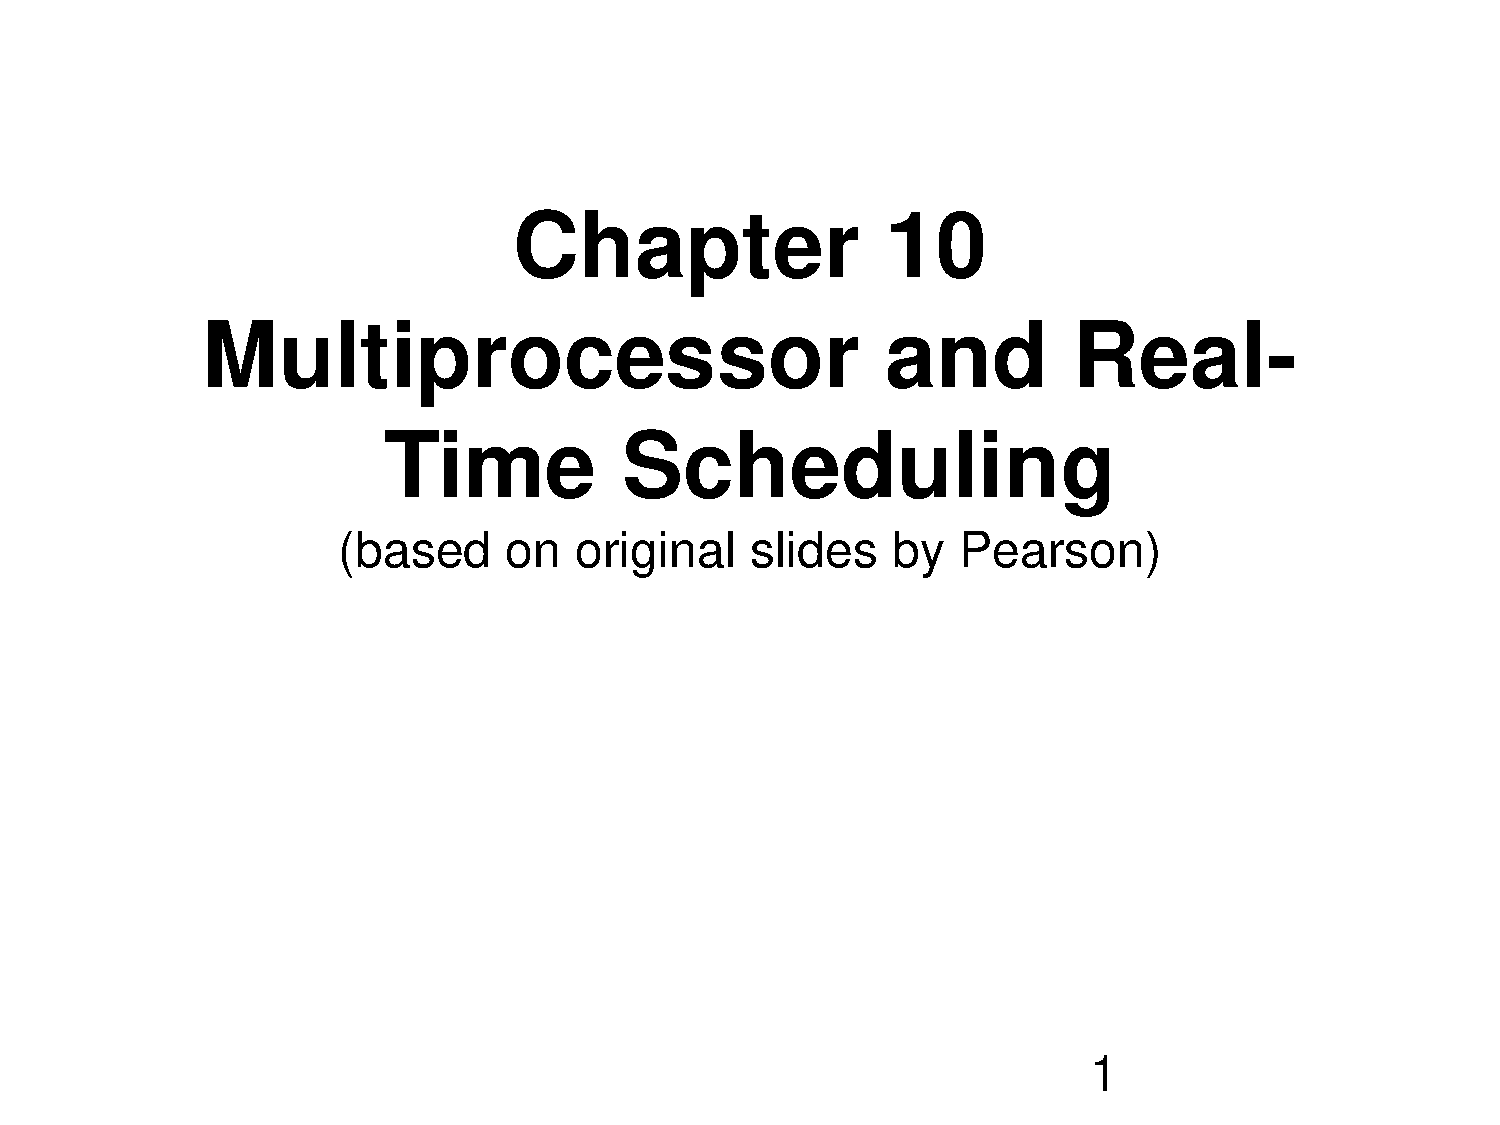
\includepdf[page=24]{10.pdf}
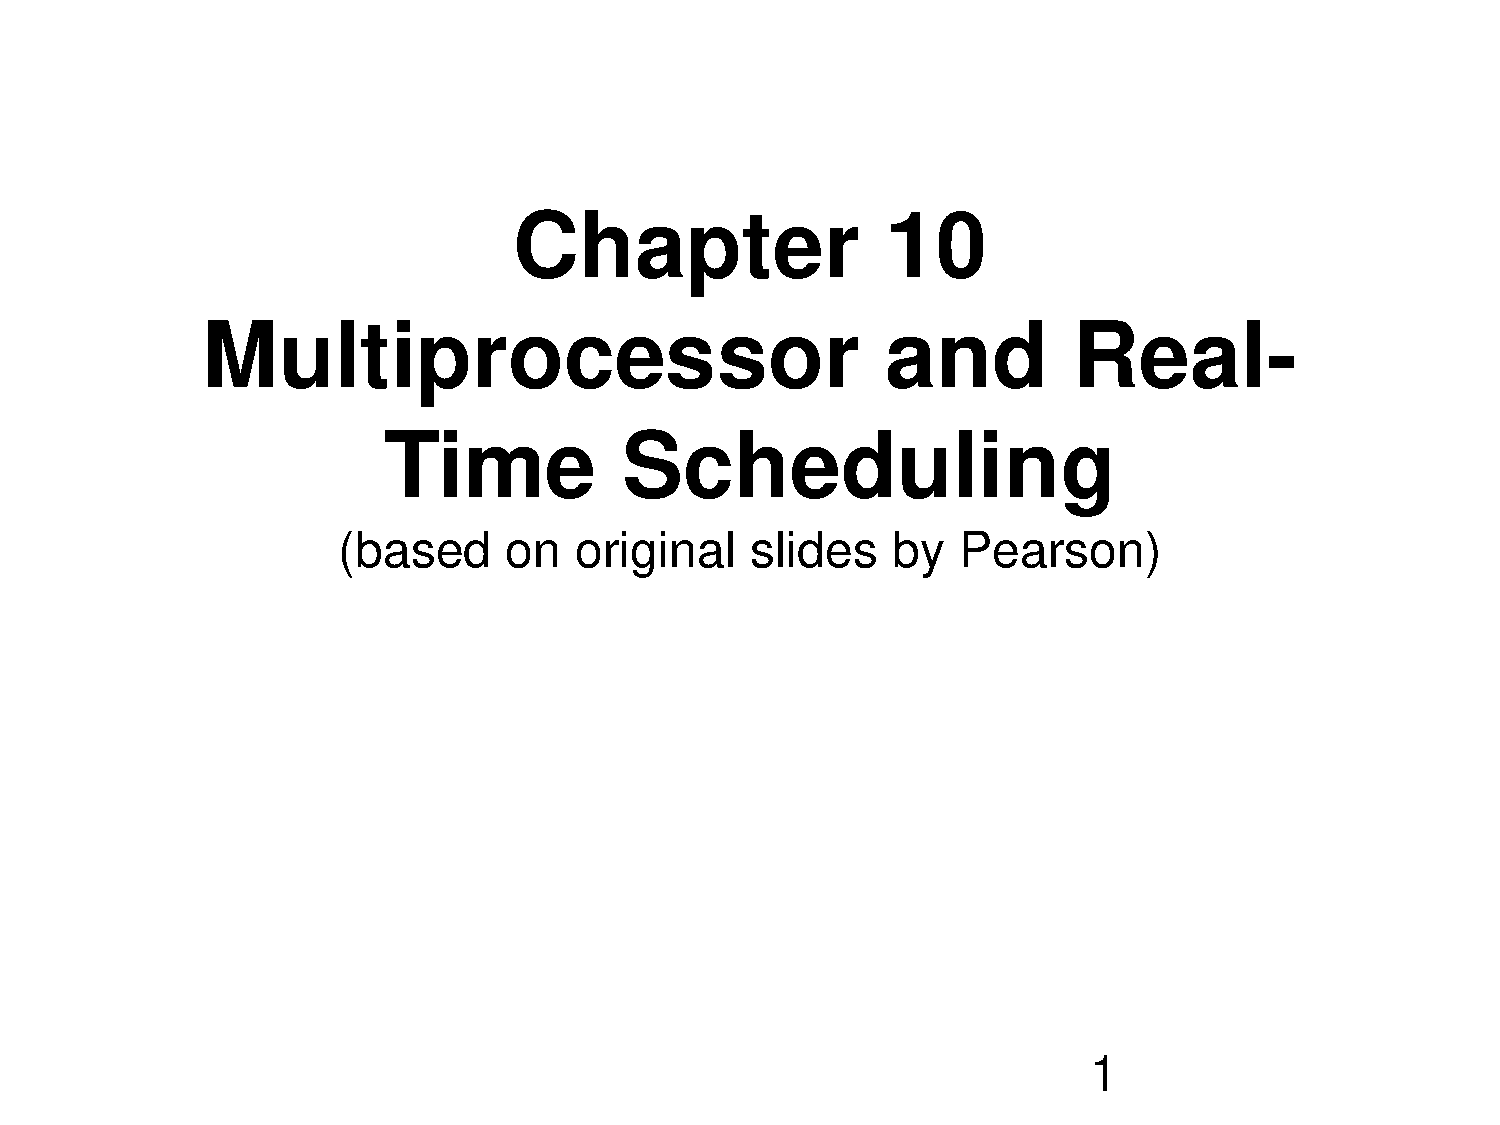
\includepdf[page=25]{10.pdf}
Consider four cores and two groups. If each group gets the same amount of time on the CPU we have some inefficiencies where the smaller group leaves its core idle. If we instead give weights to each group and allocate CPU time based on that we get better efficiency.
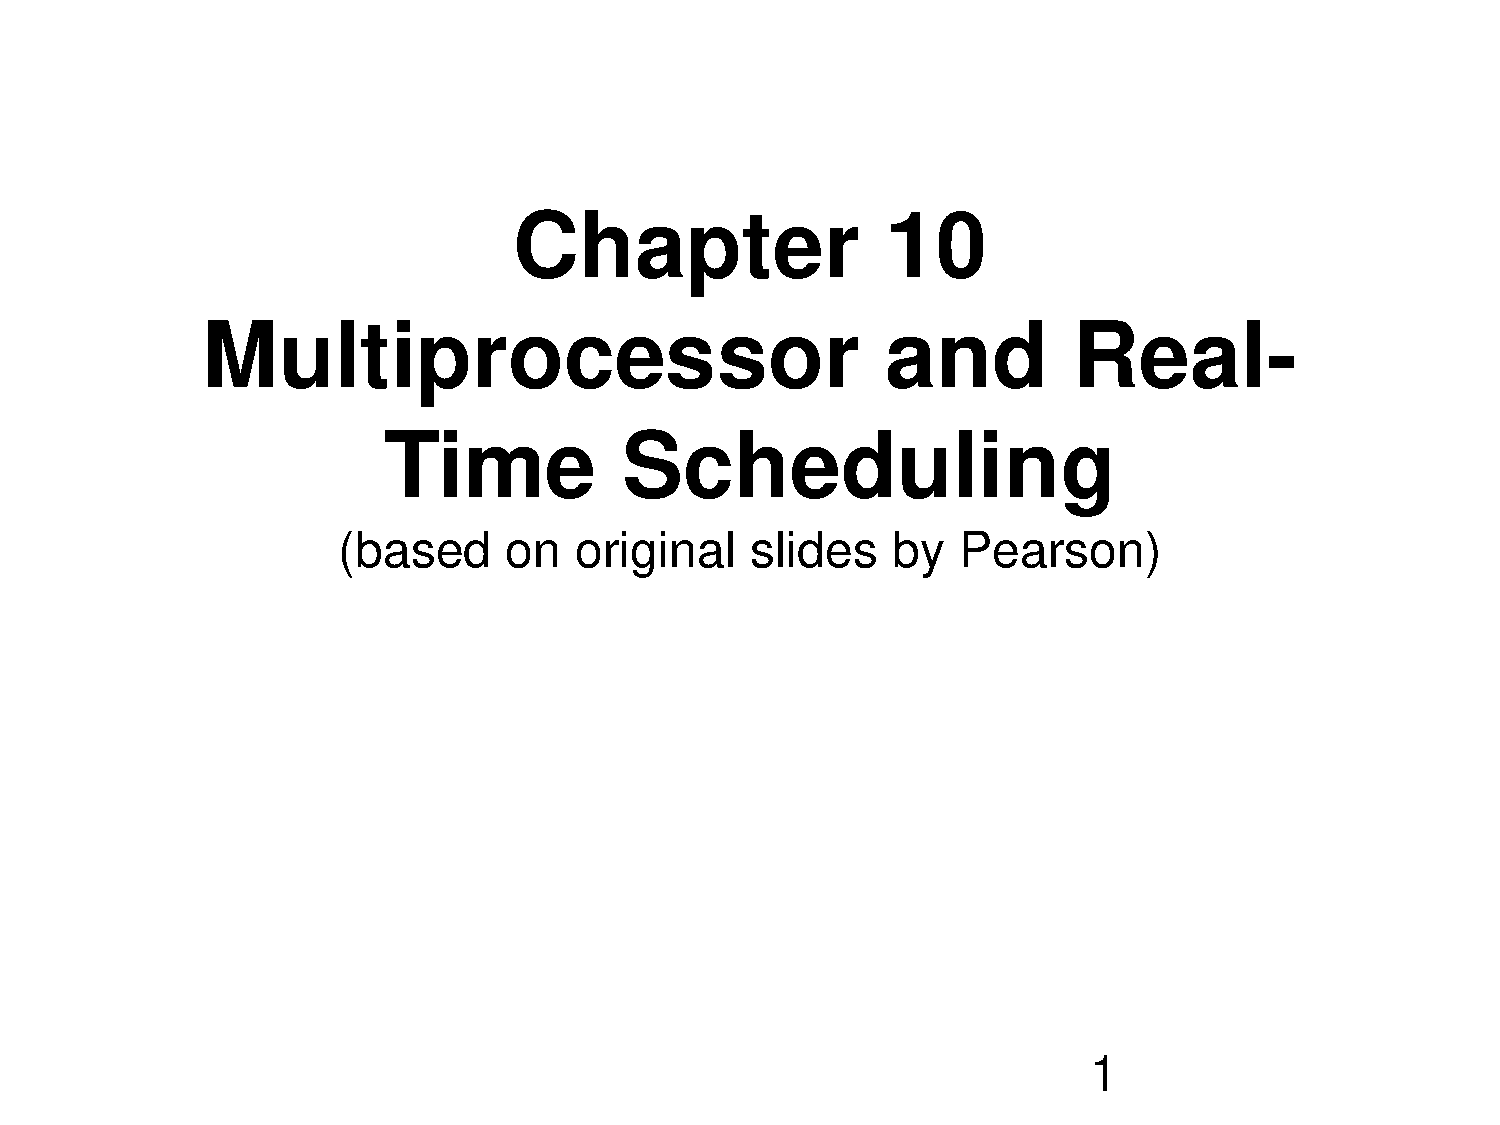
\includepdf[page=26]{10.pdf}
Here we have a group take a core until it is done. This is beneficial because there is no overhead from switching, but also inefficient because there is no more multiprogramming.
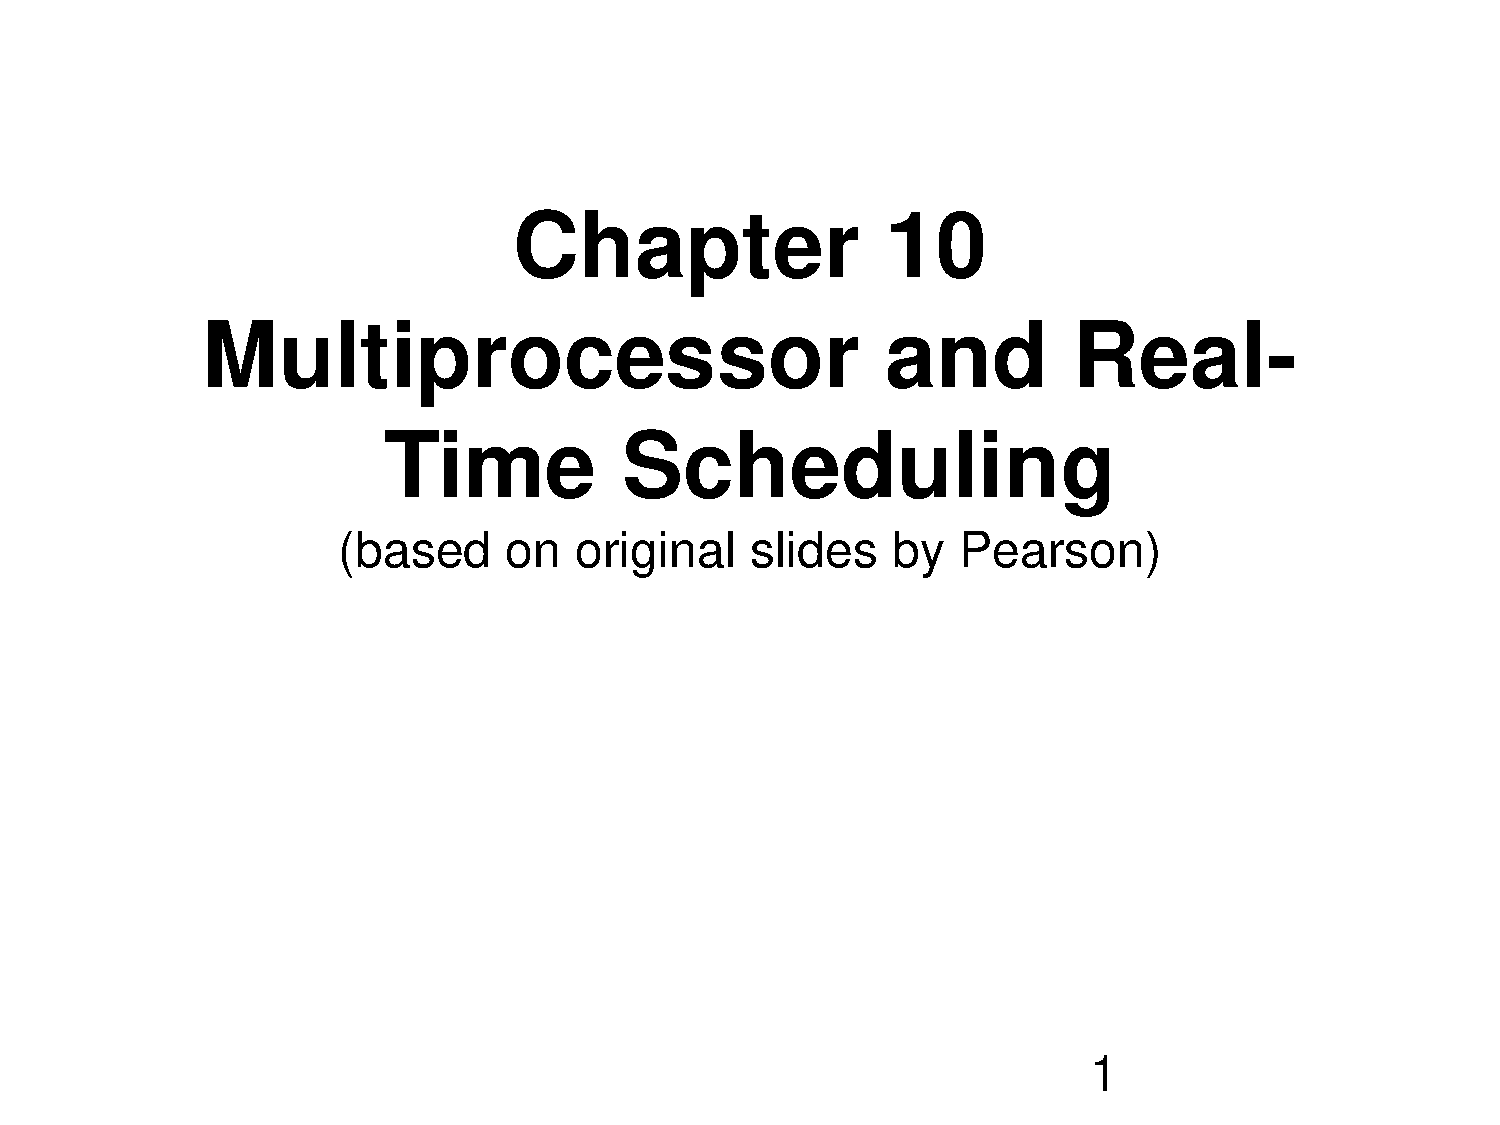
\includepdf[page=27]{10.pdf}
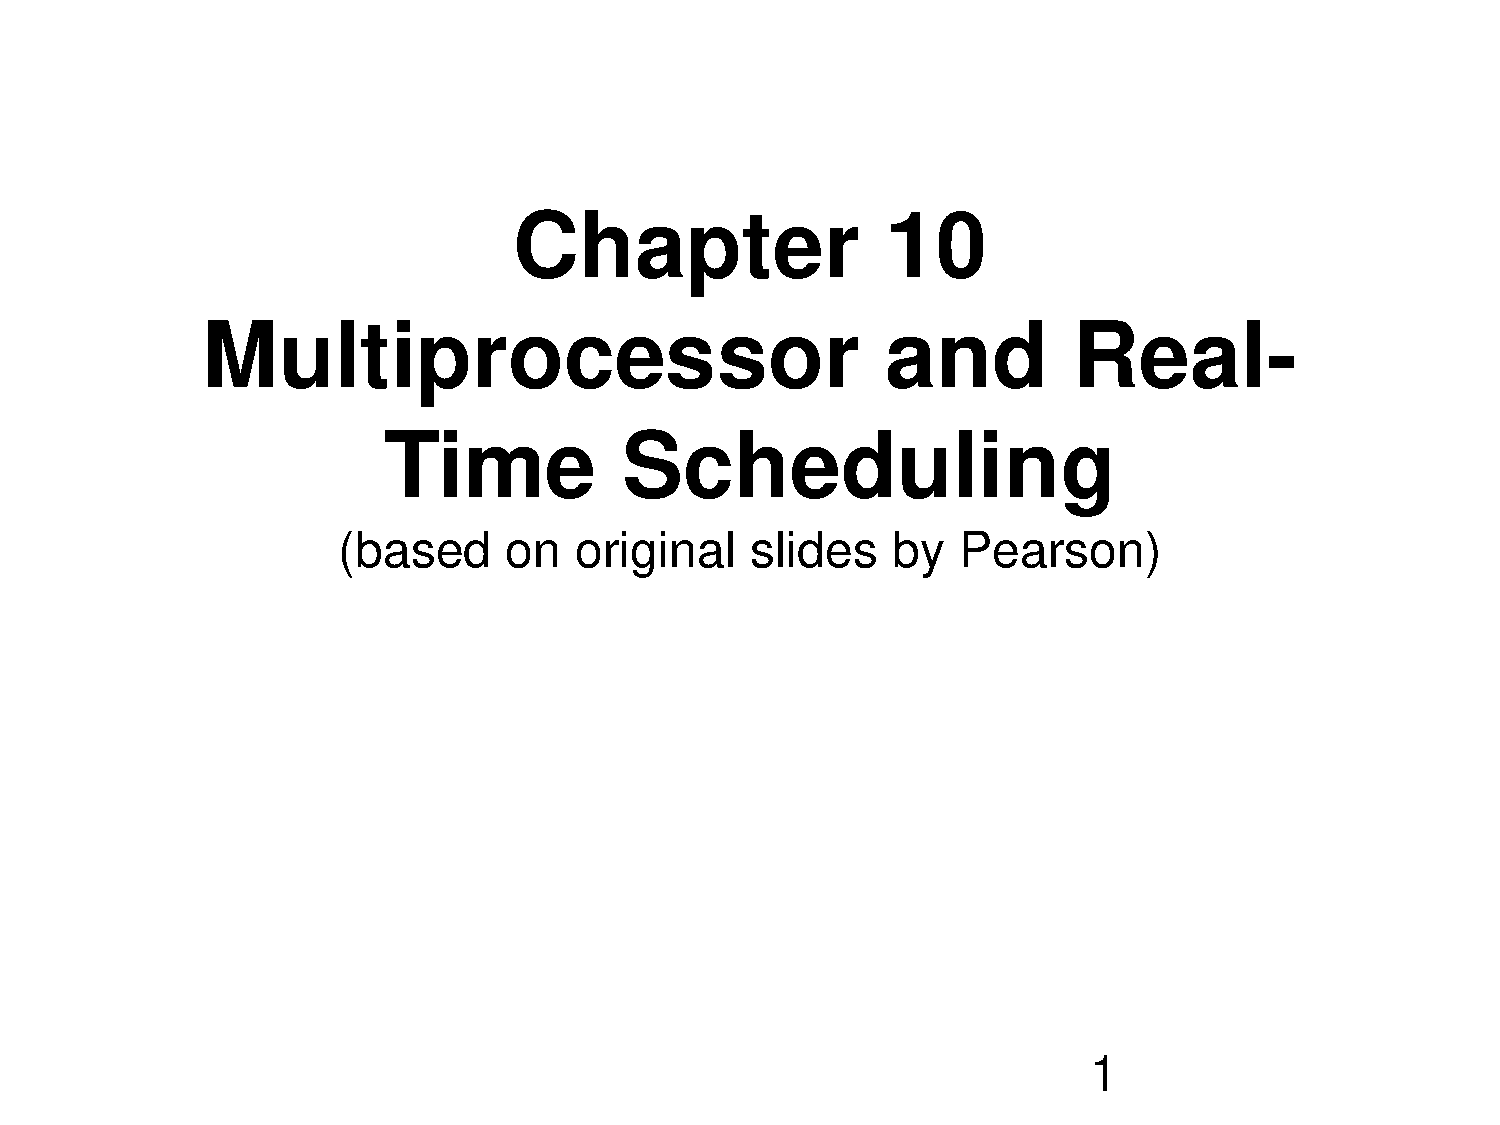
\includepdf[page=28]{10.pdf}
The user can alter the number of threads in your application.
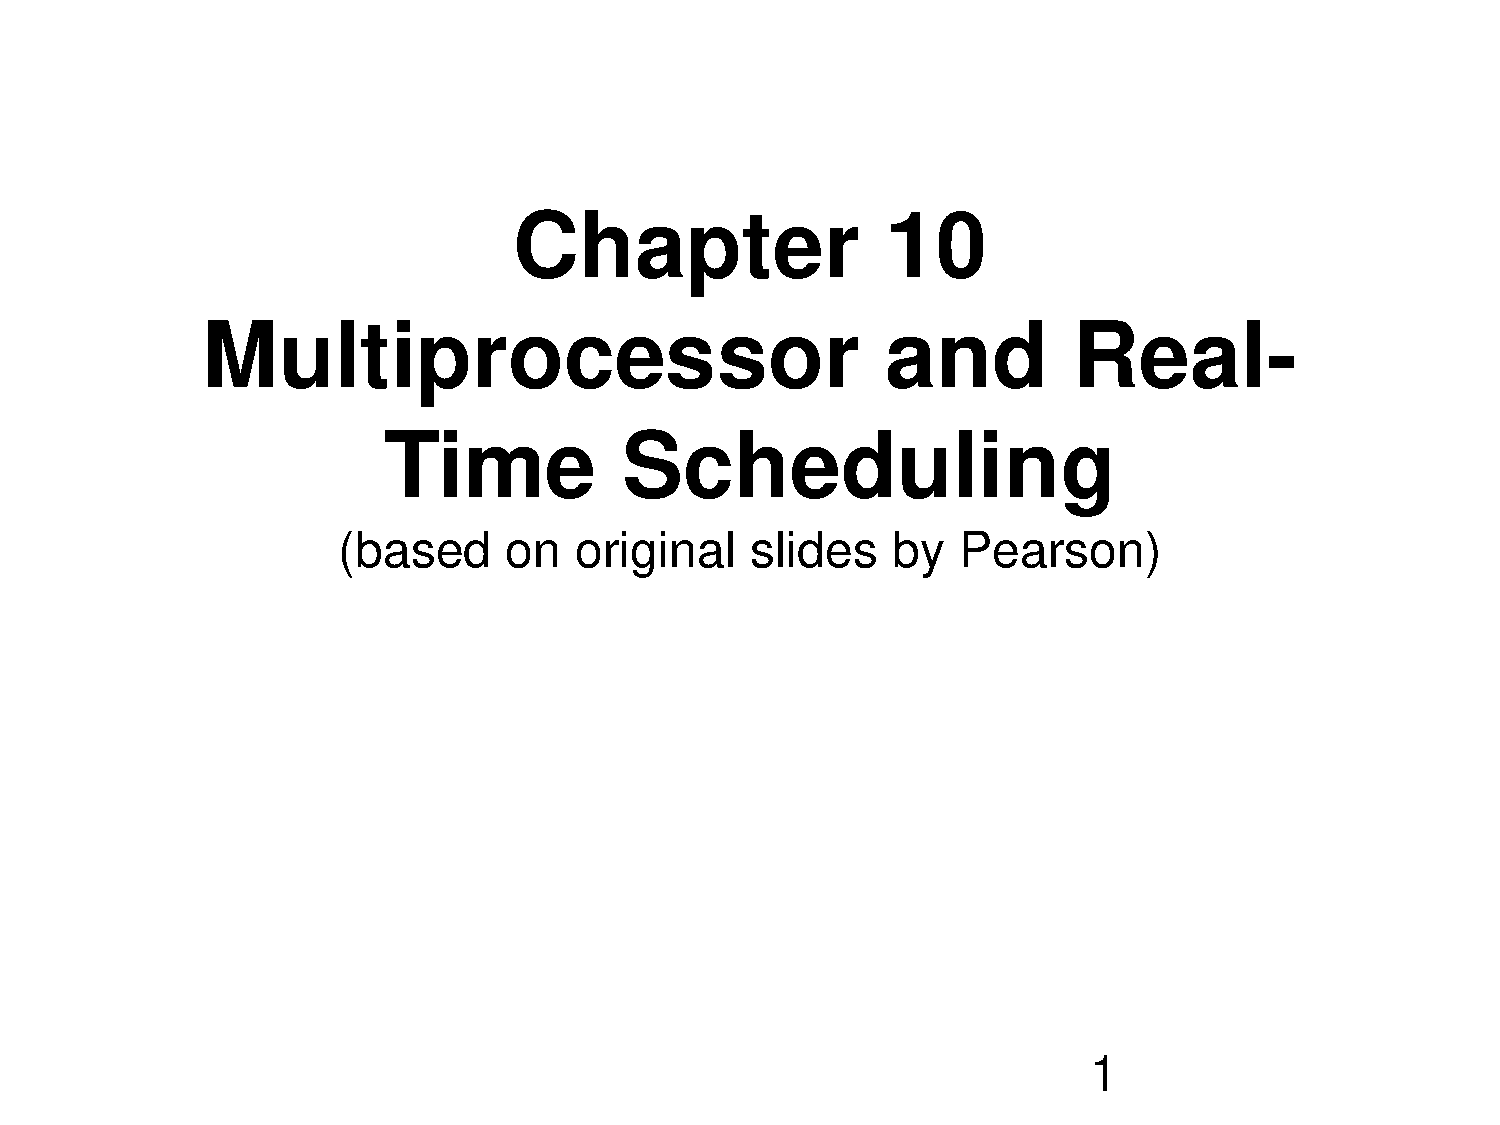
\includepdf[page=29]{10.pdf}
Now the correctness of a system is not based on logic, but timing as well.
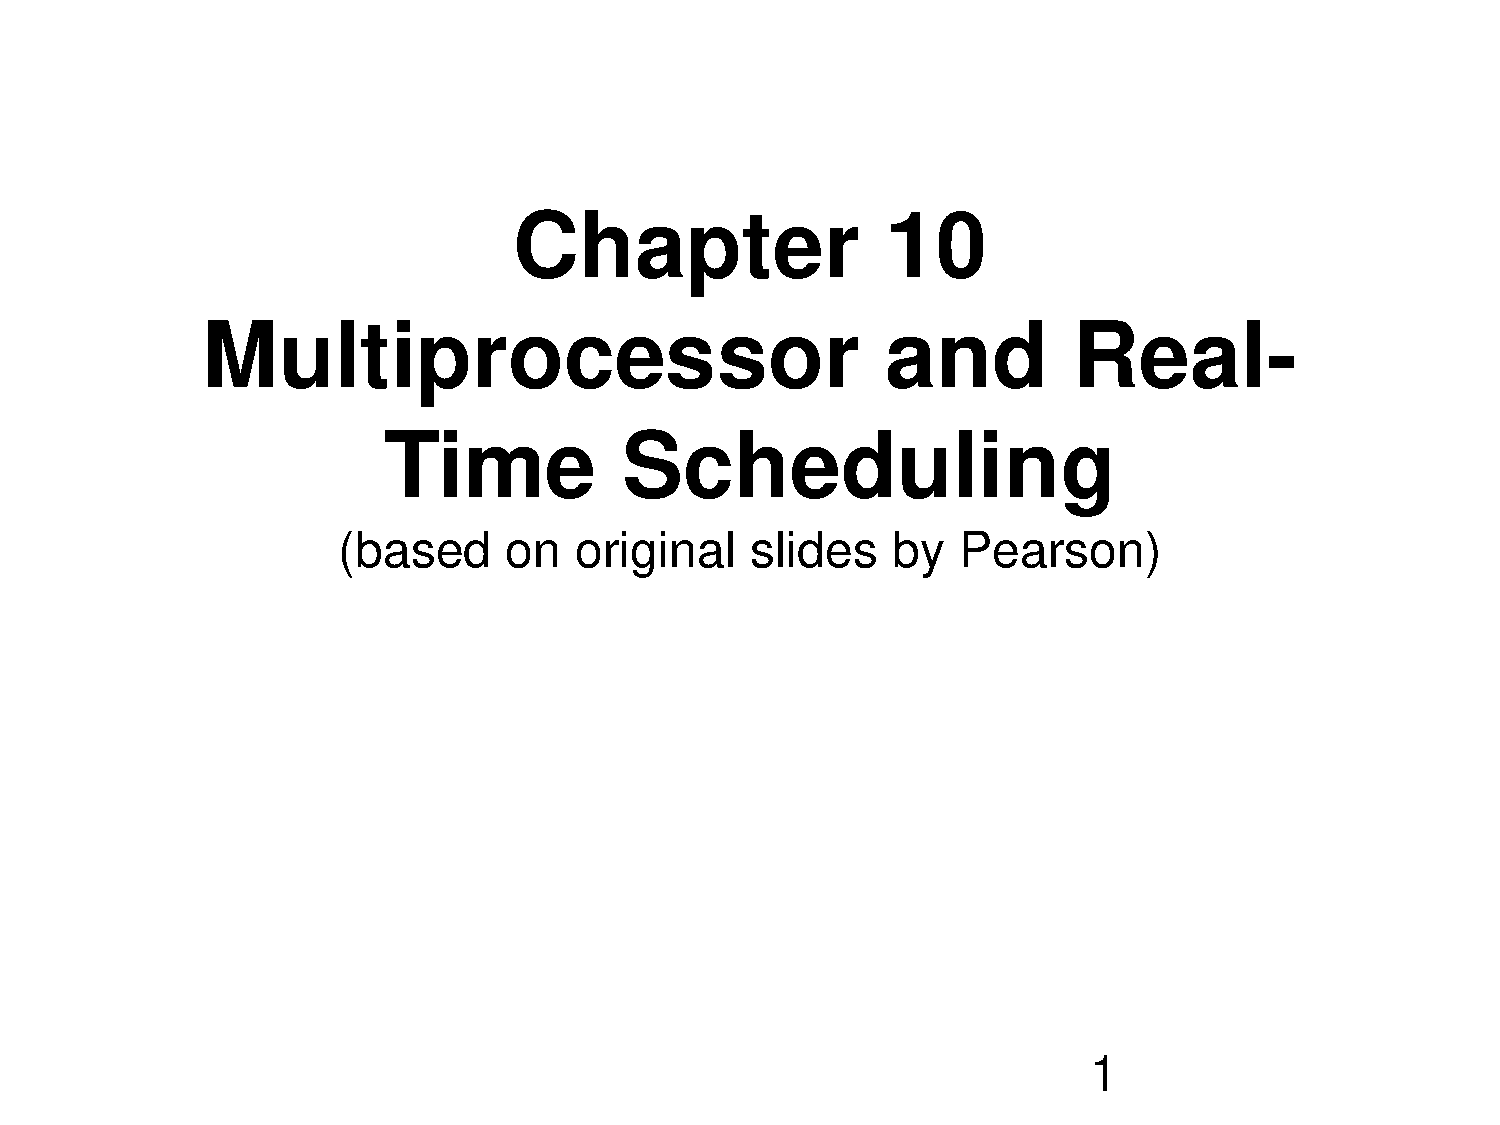
\includepdf[page=30]{10.pdf}
We have to produce the correct result at the correct time. This results in tempral constrants being used to specify when a result is on time.
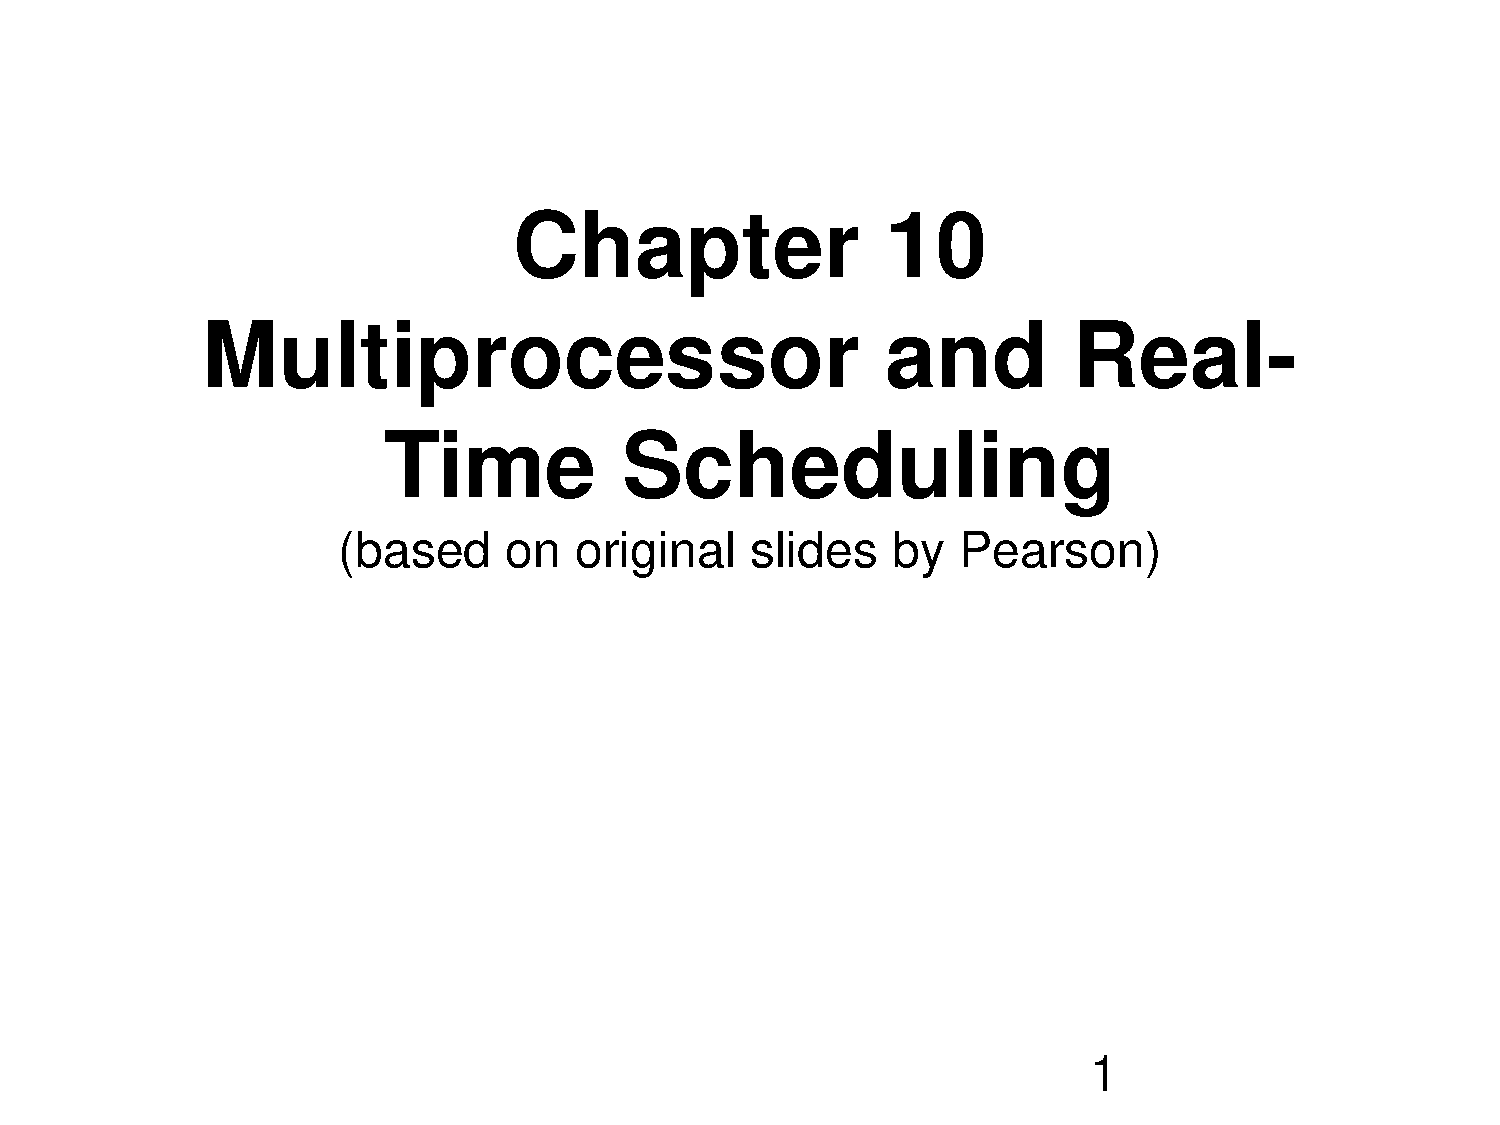
\includepdf[page=31]{10.pdf}
Soft real time systems - temproal constraints looks at the average response time. Arriving late occasionally is not bad but frequent lates is really shitty.
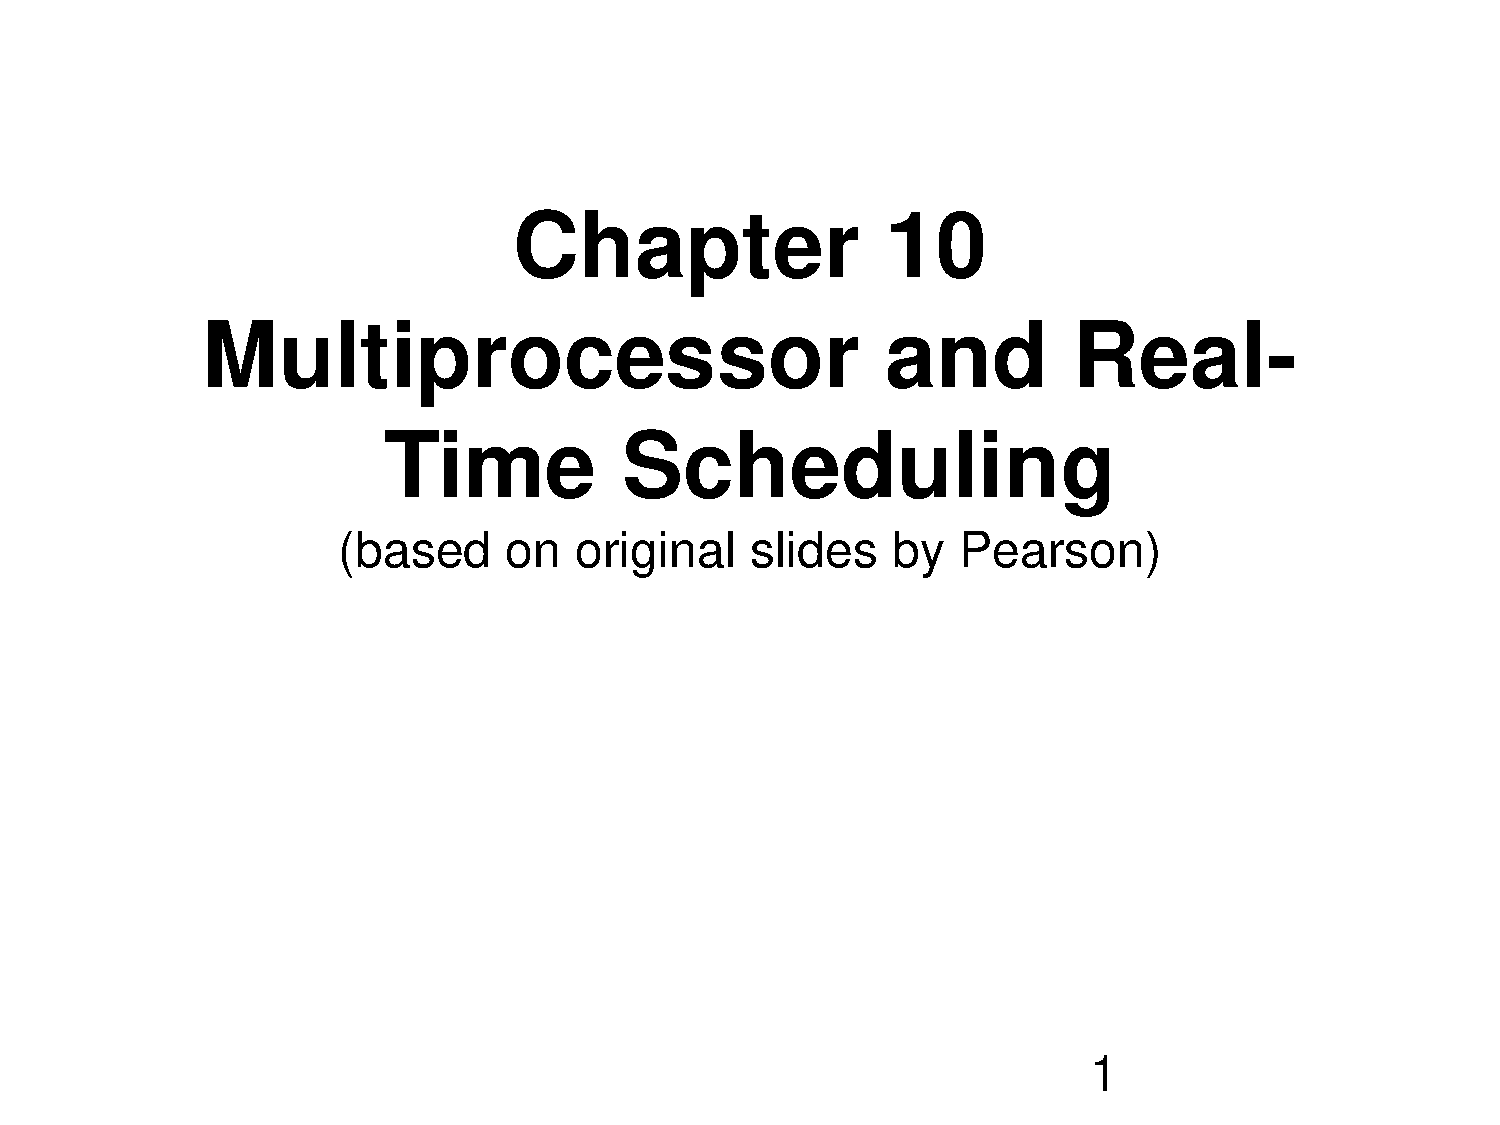
\includepdf[page=32]{10.pdf}
Hard real time systems - everything must absolutely be on time (withing a range)
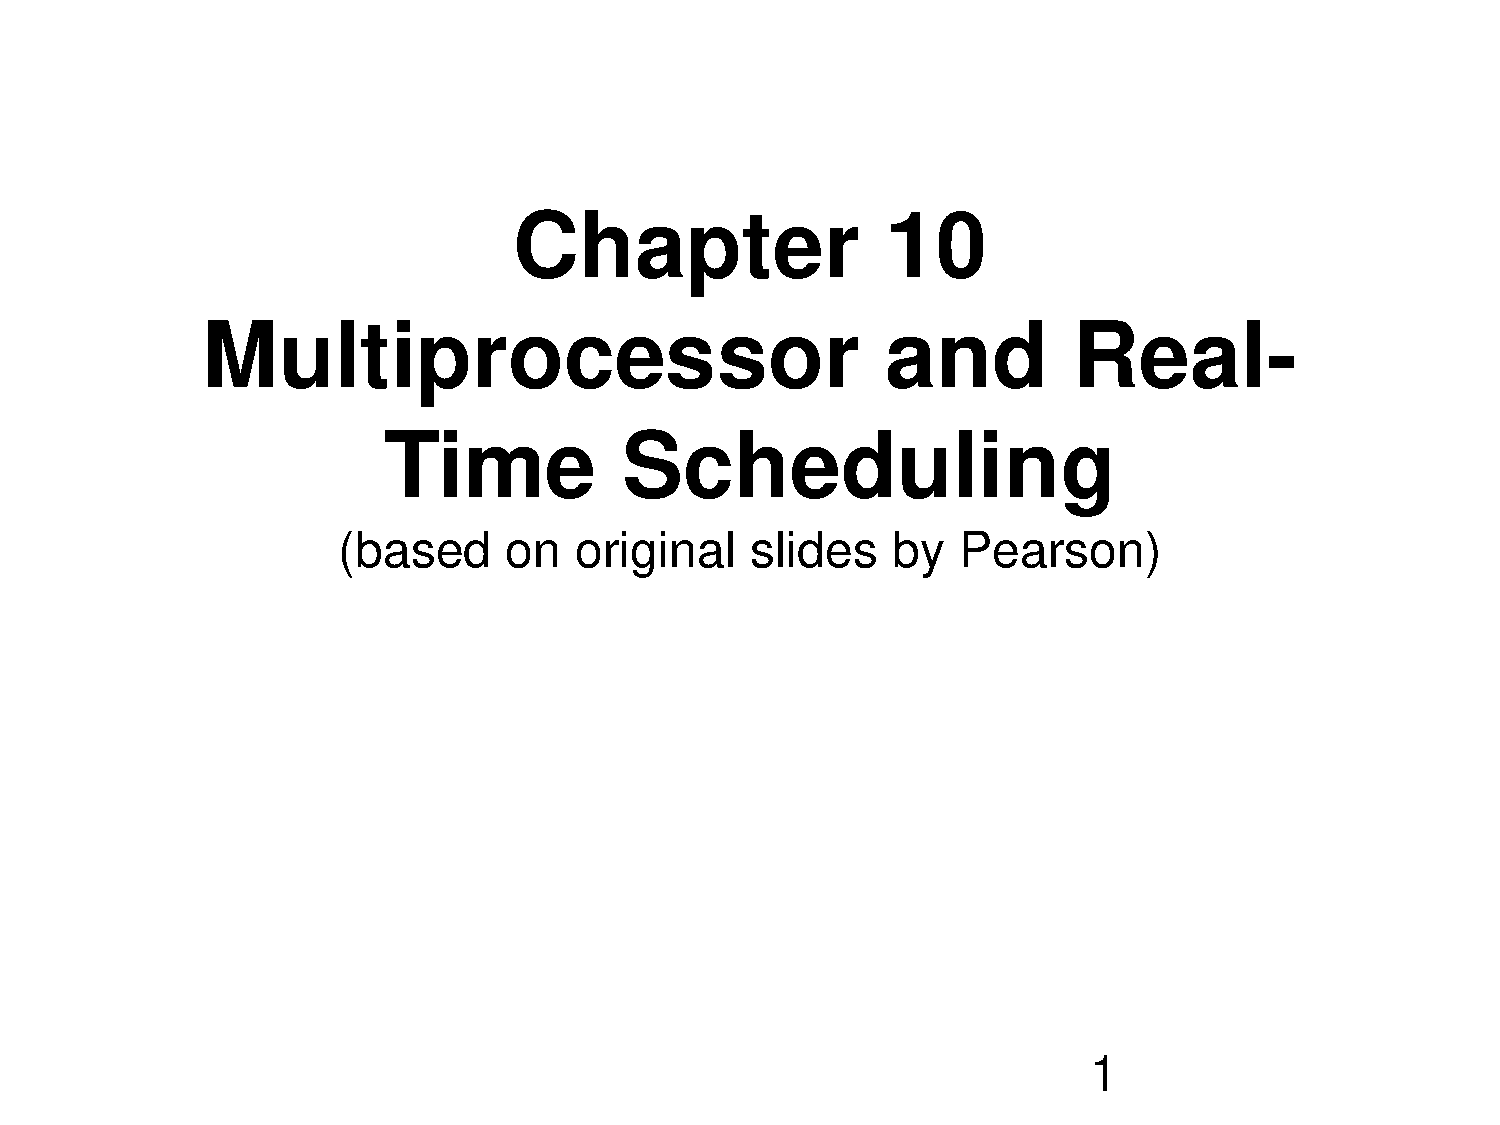
\includepdf[page=33]{10.pdf}
Firm temporal constraints are a combination of hard and soft.
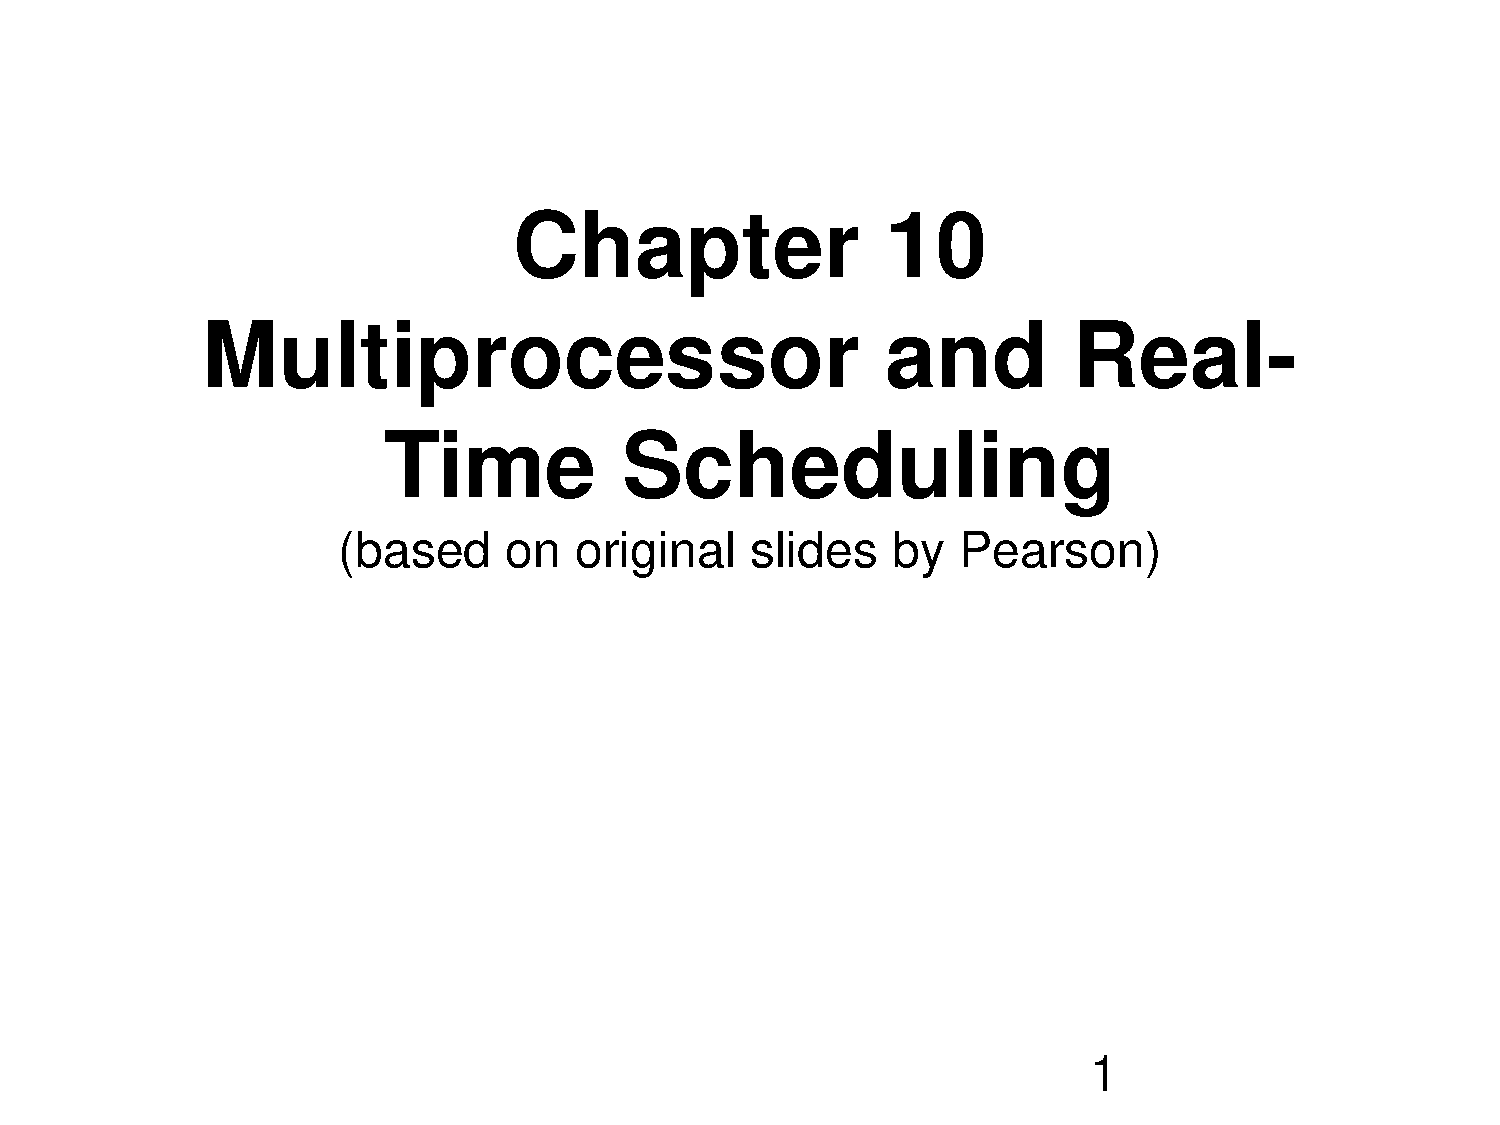
\includepdf[page=34]{10.pdf}
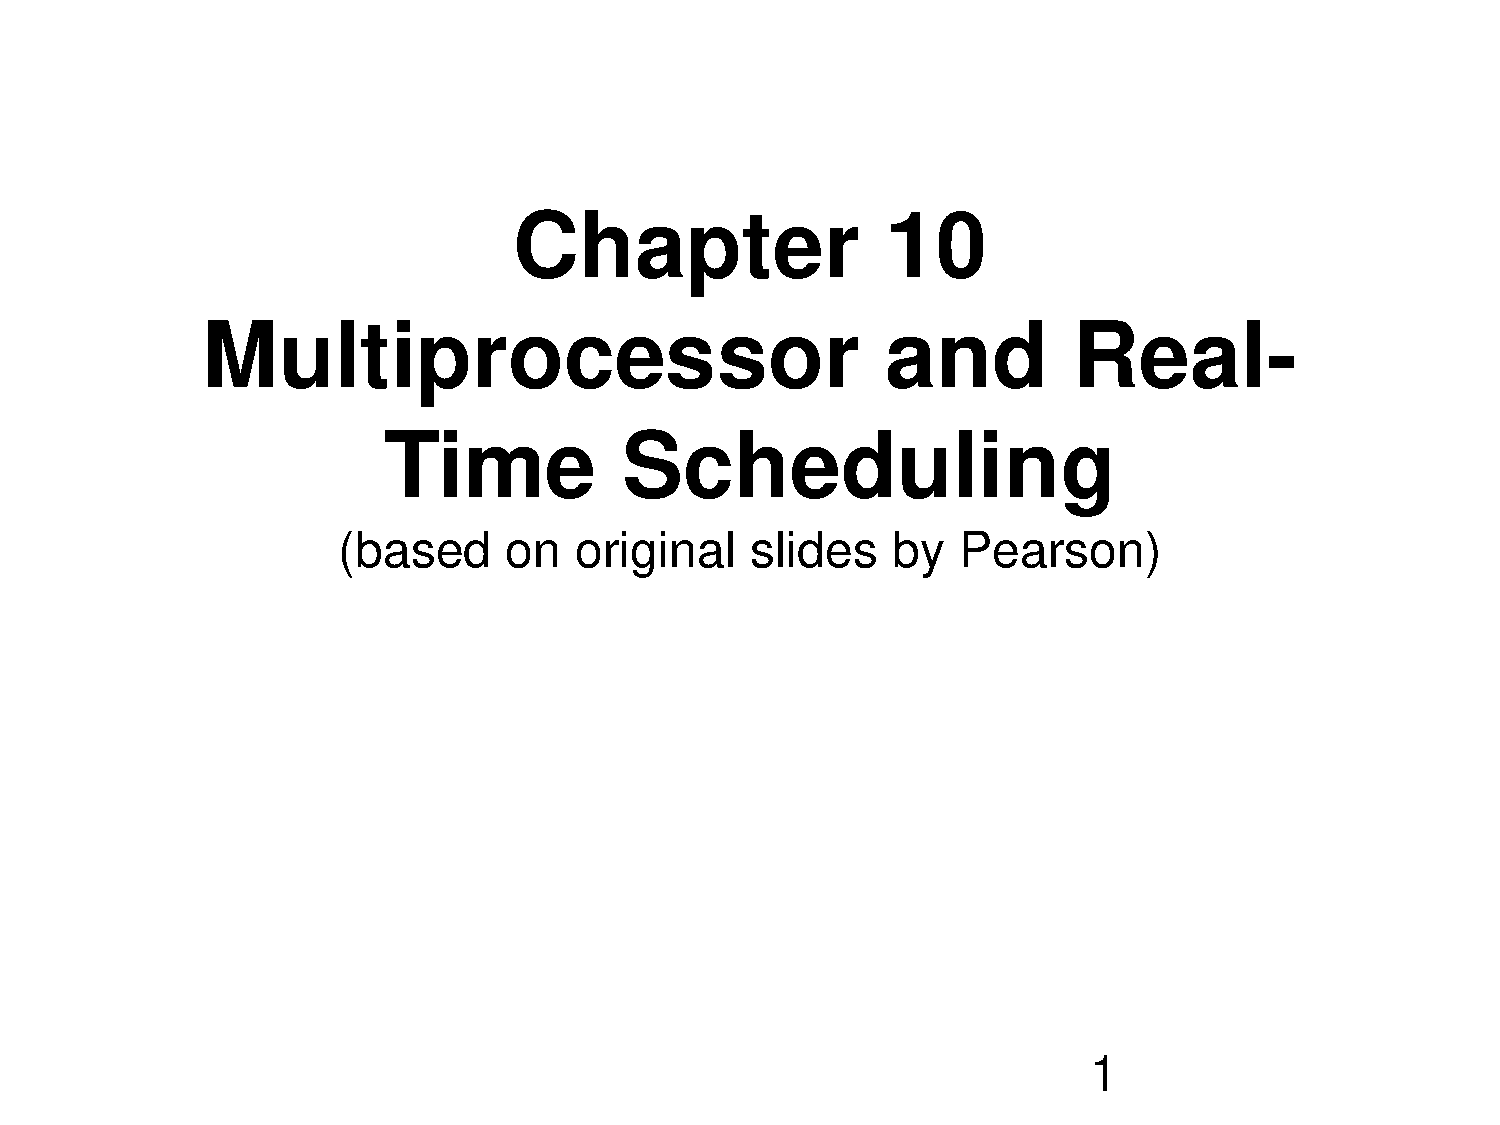
\includepdf[page=35]{10.pdf}
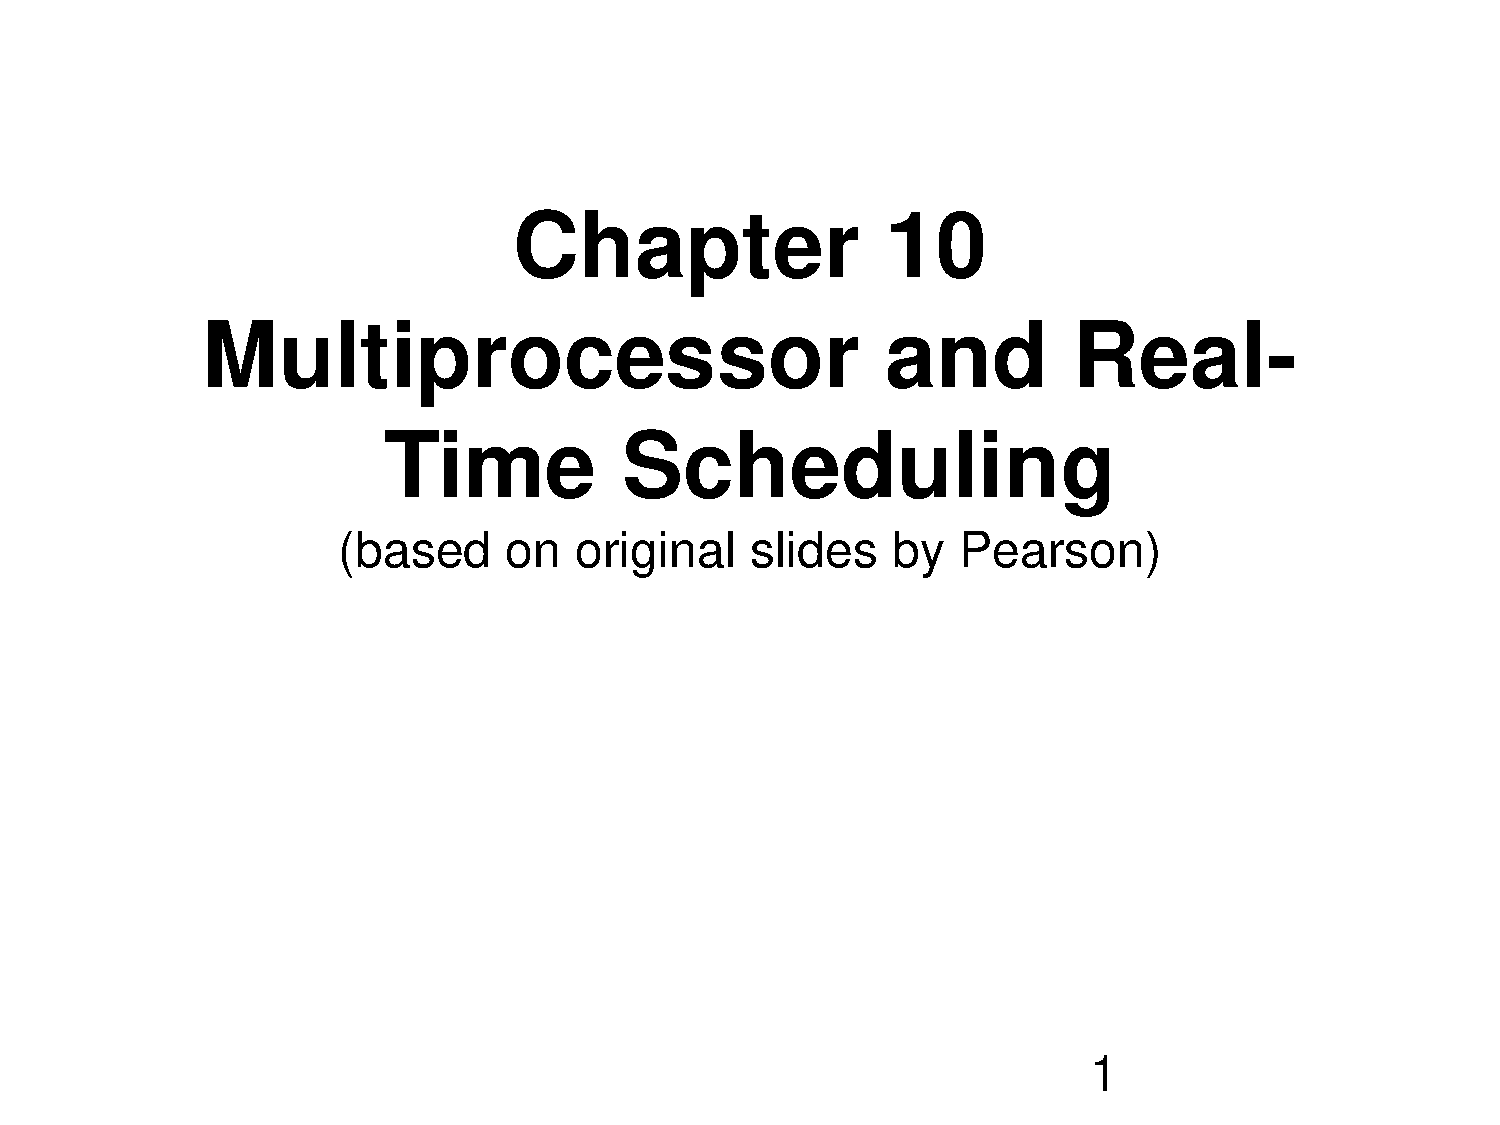
\includepdf[page=36]{10.pdf}
Responsiveness is how long the interrupt handler takes to deal with an event.
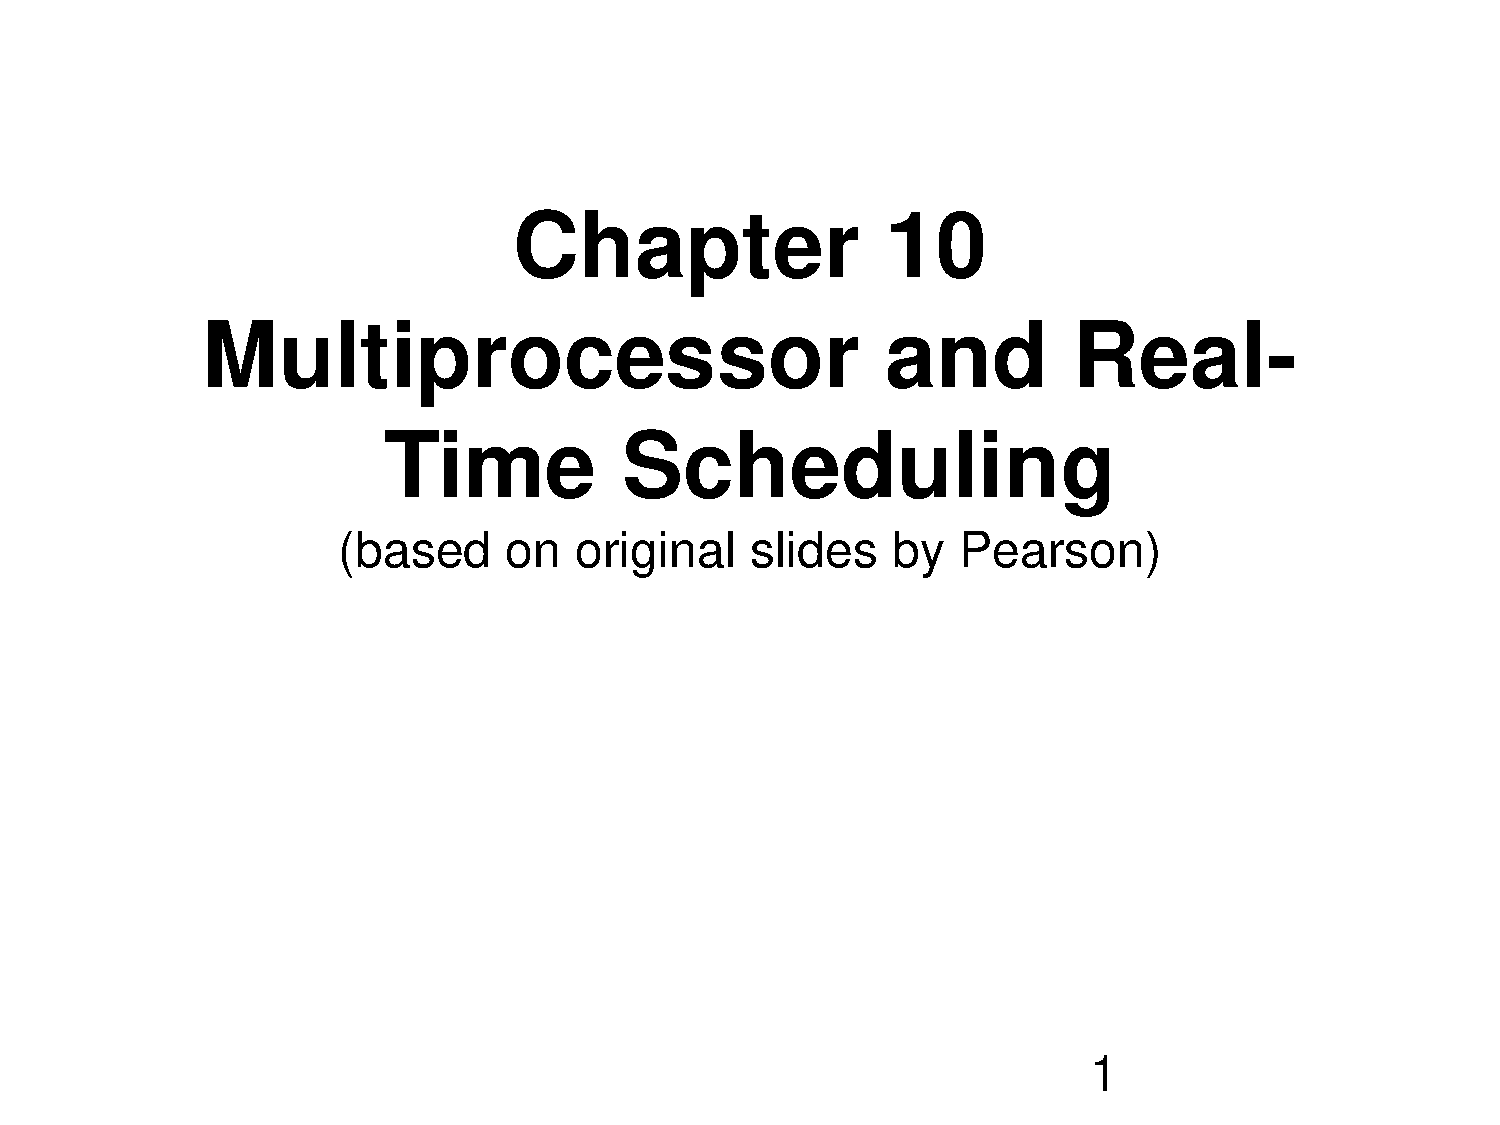
\includepdf[page=37]{10.pdf}
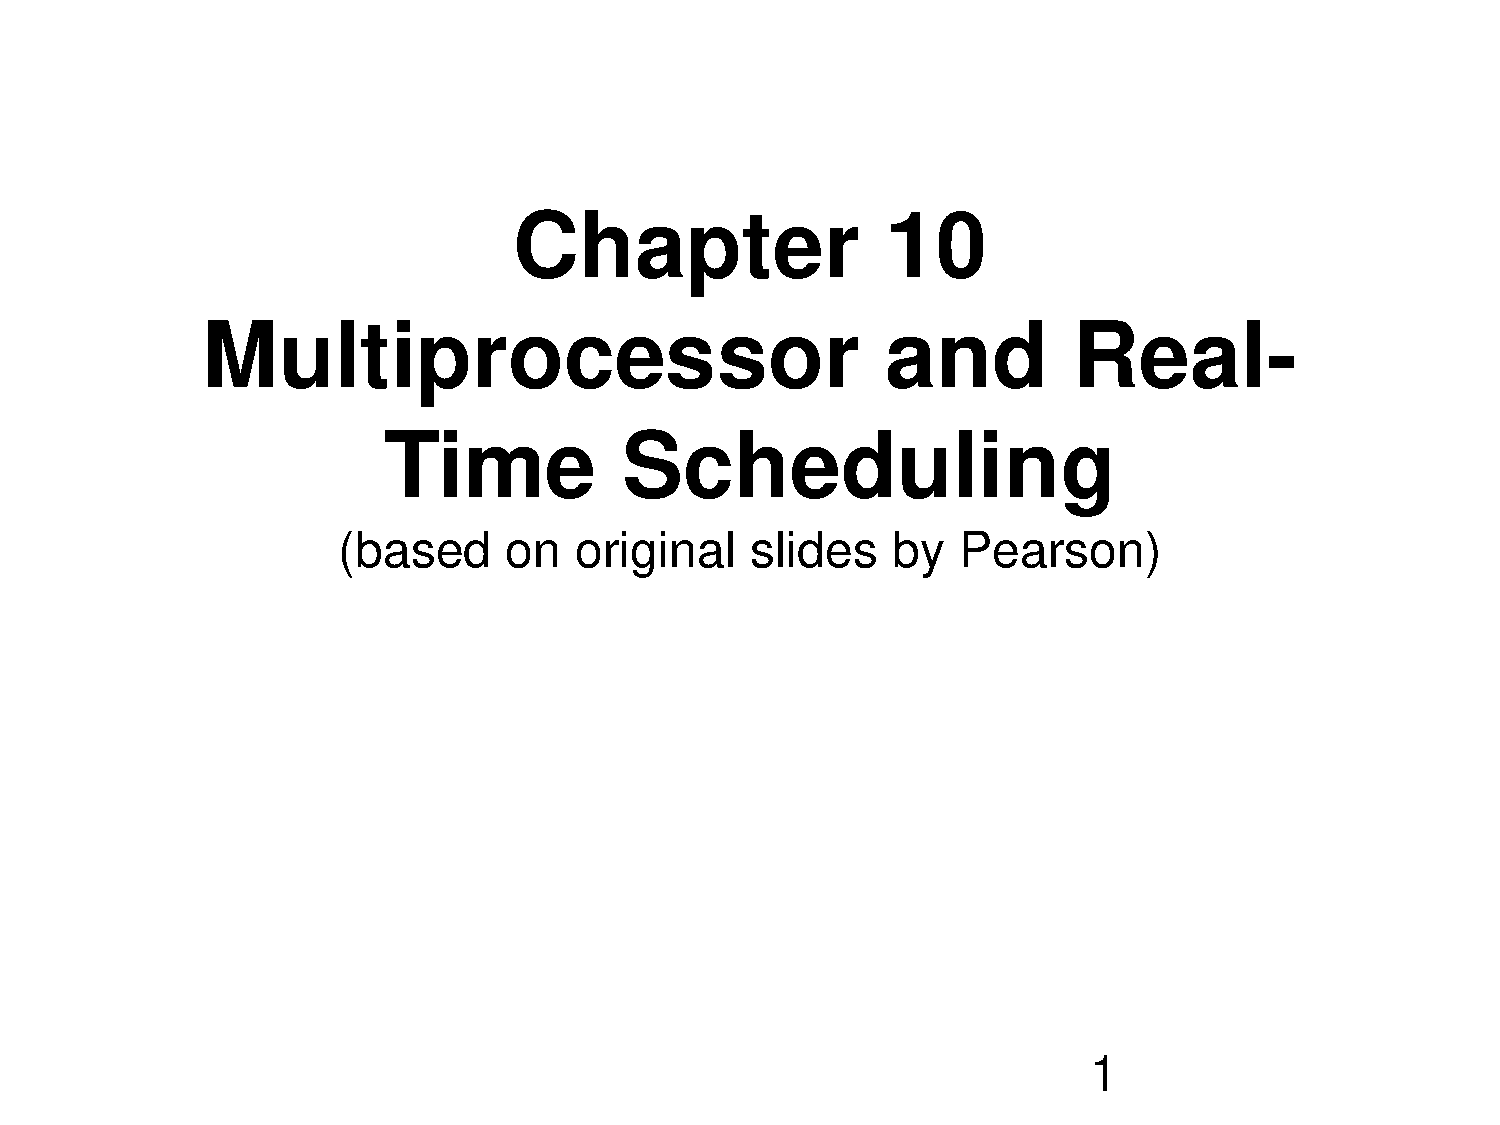
\includepdf[page=38]{10.pdf}
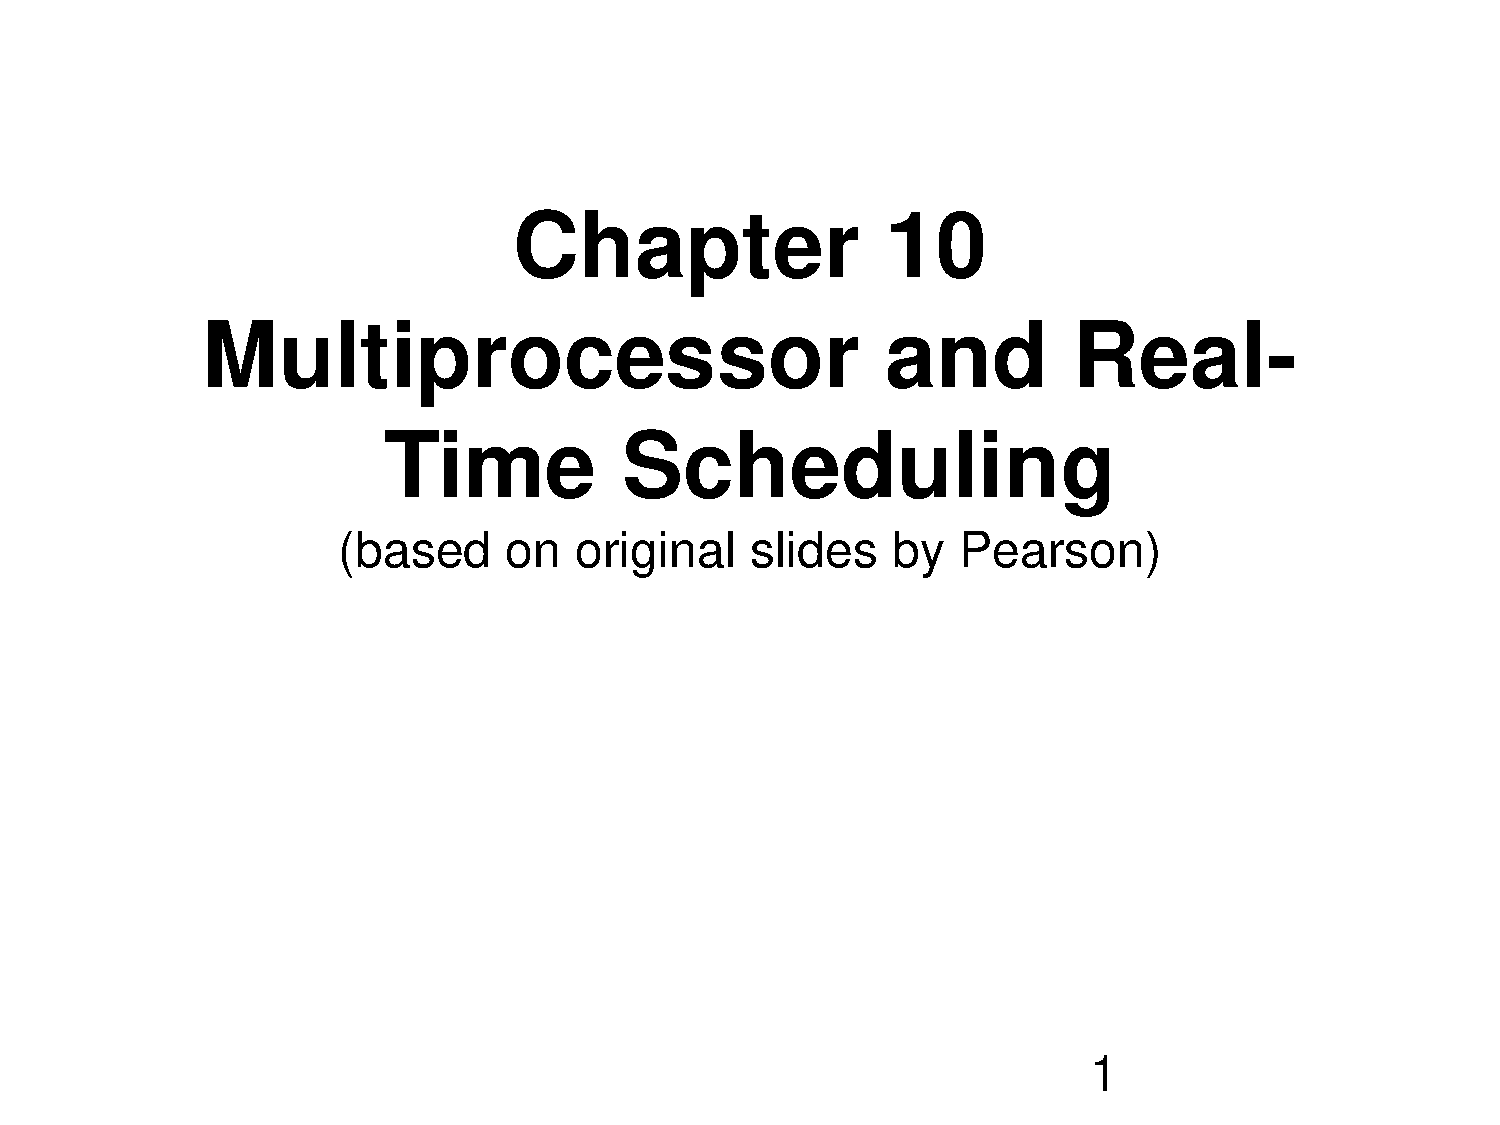
\includepdf[page=39]{10.pdf}
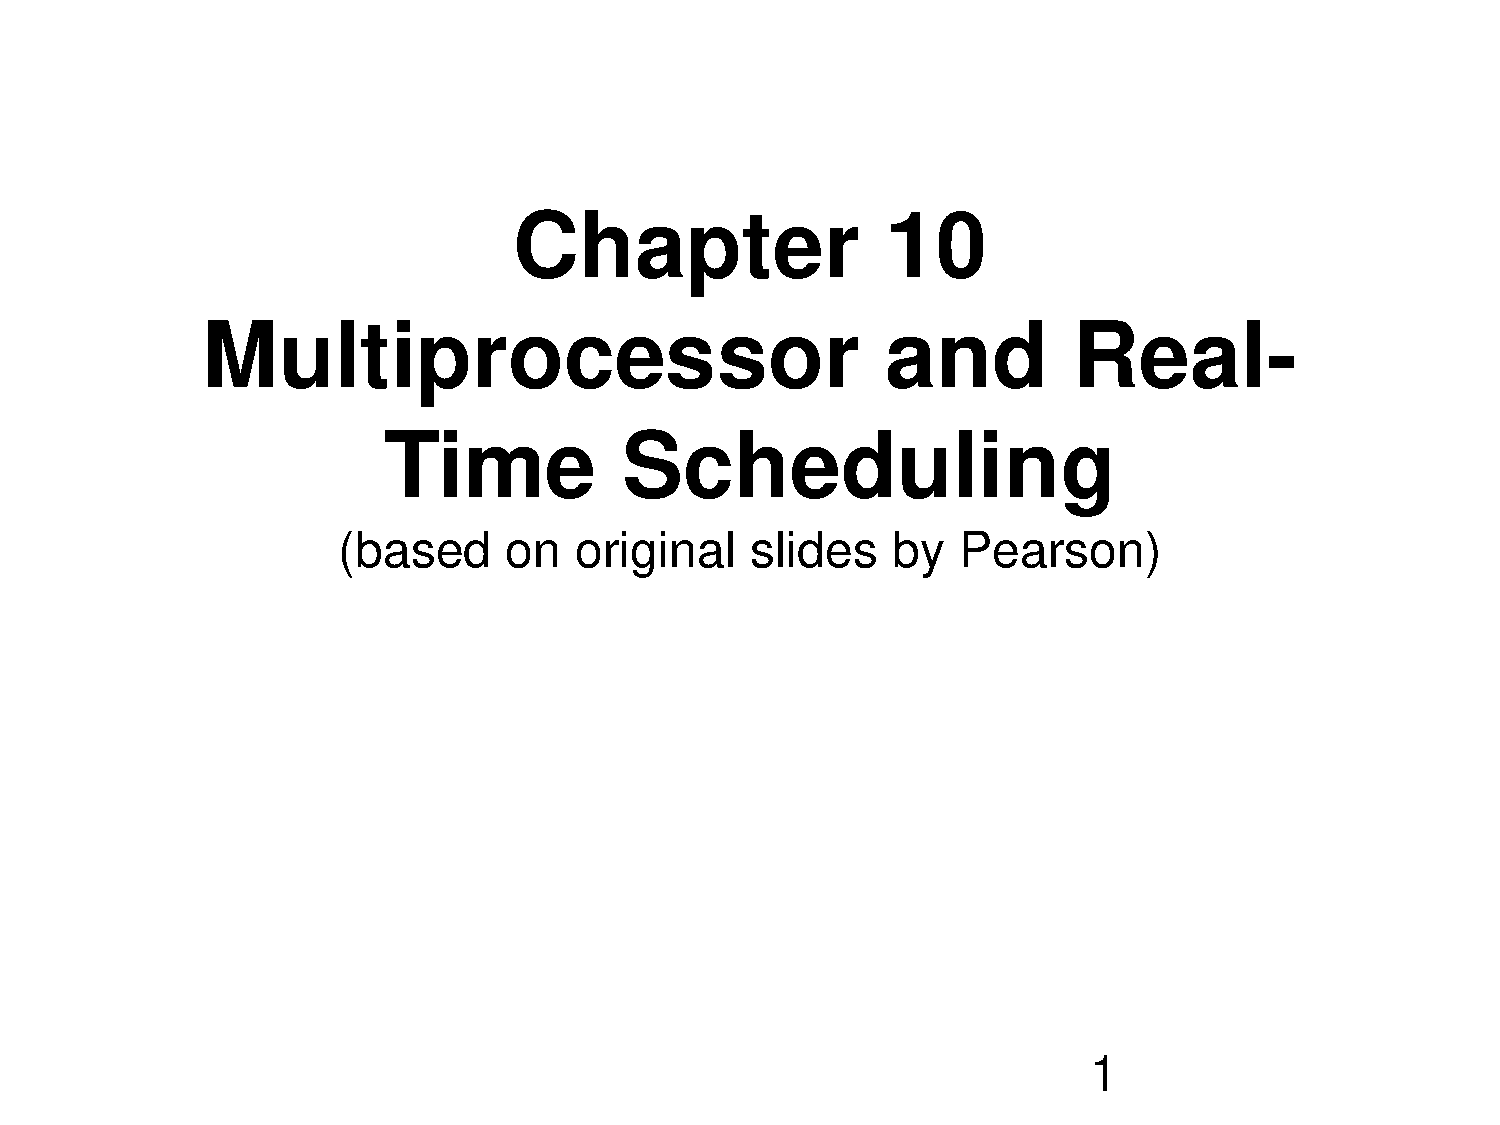
\includepdf[page=40]{10.pdf}
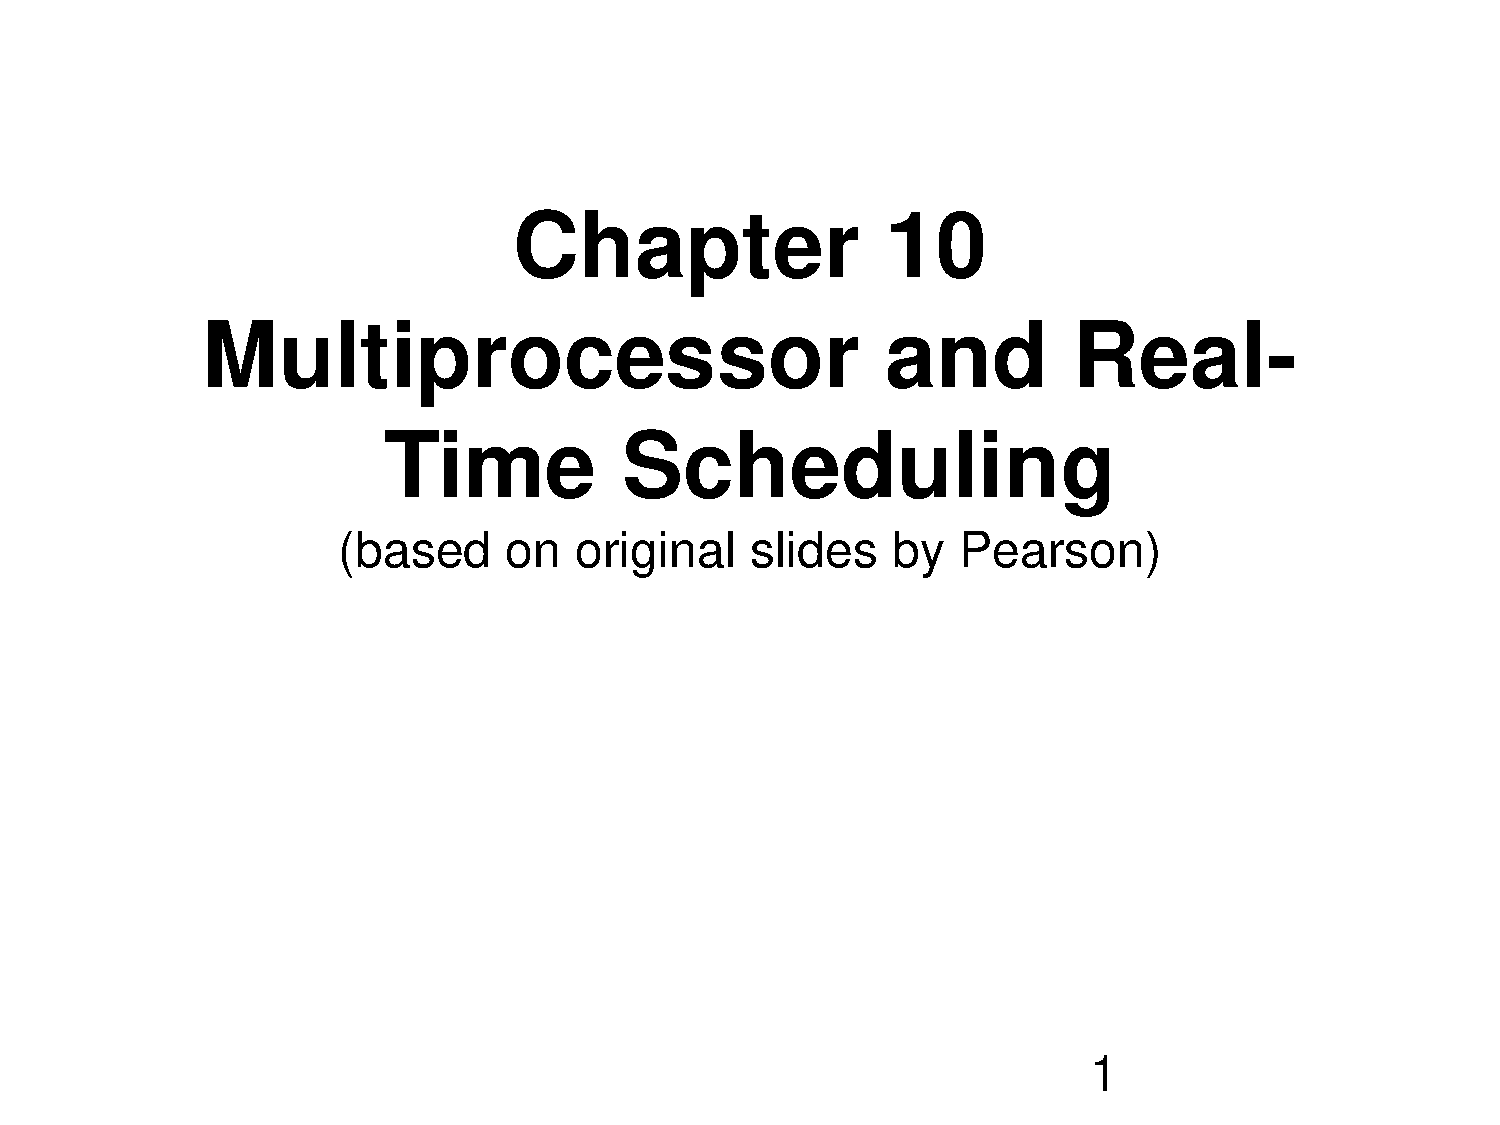
\includepdf[page=41]{10.pdf}
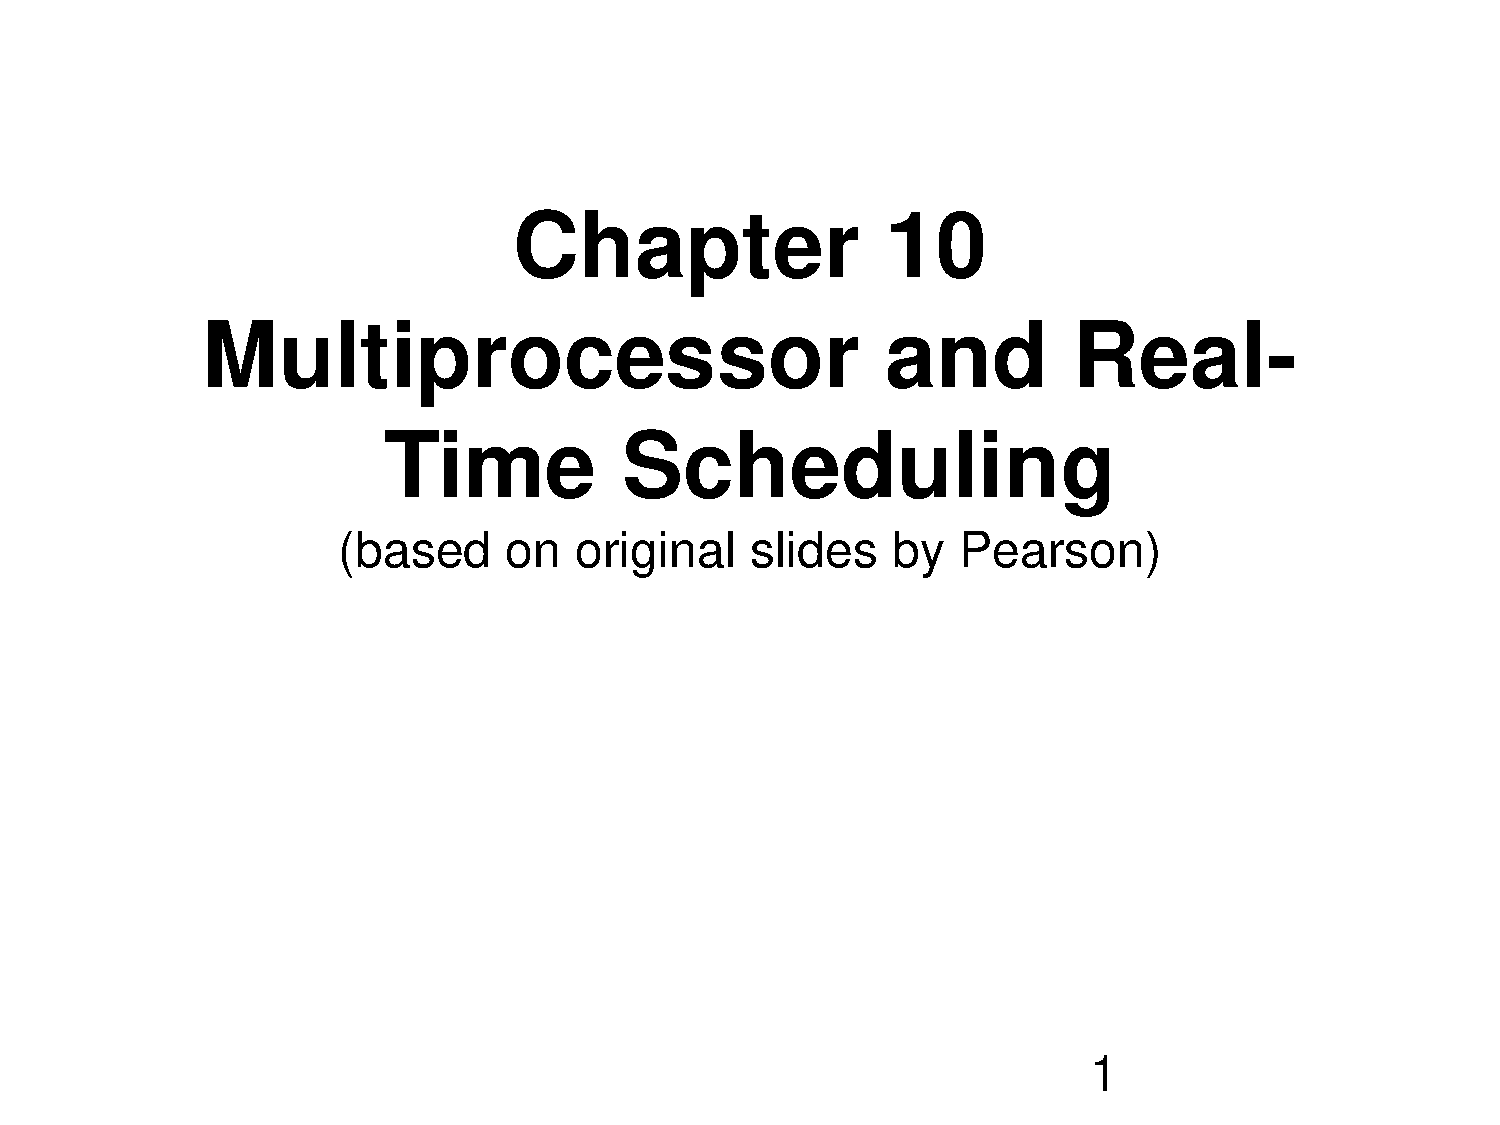
\includepdf[page=42]{10.pdf}
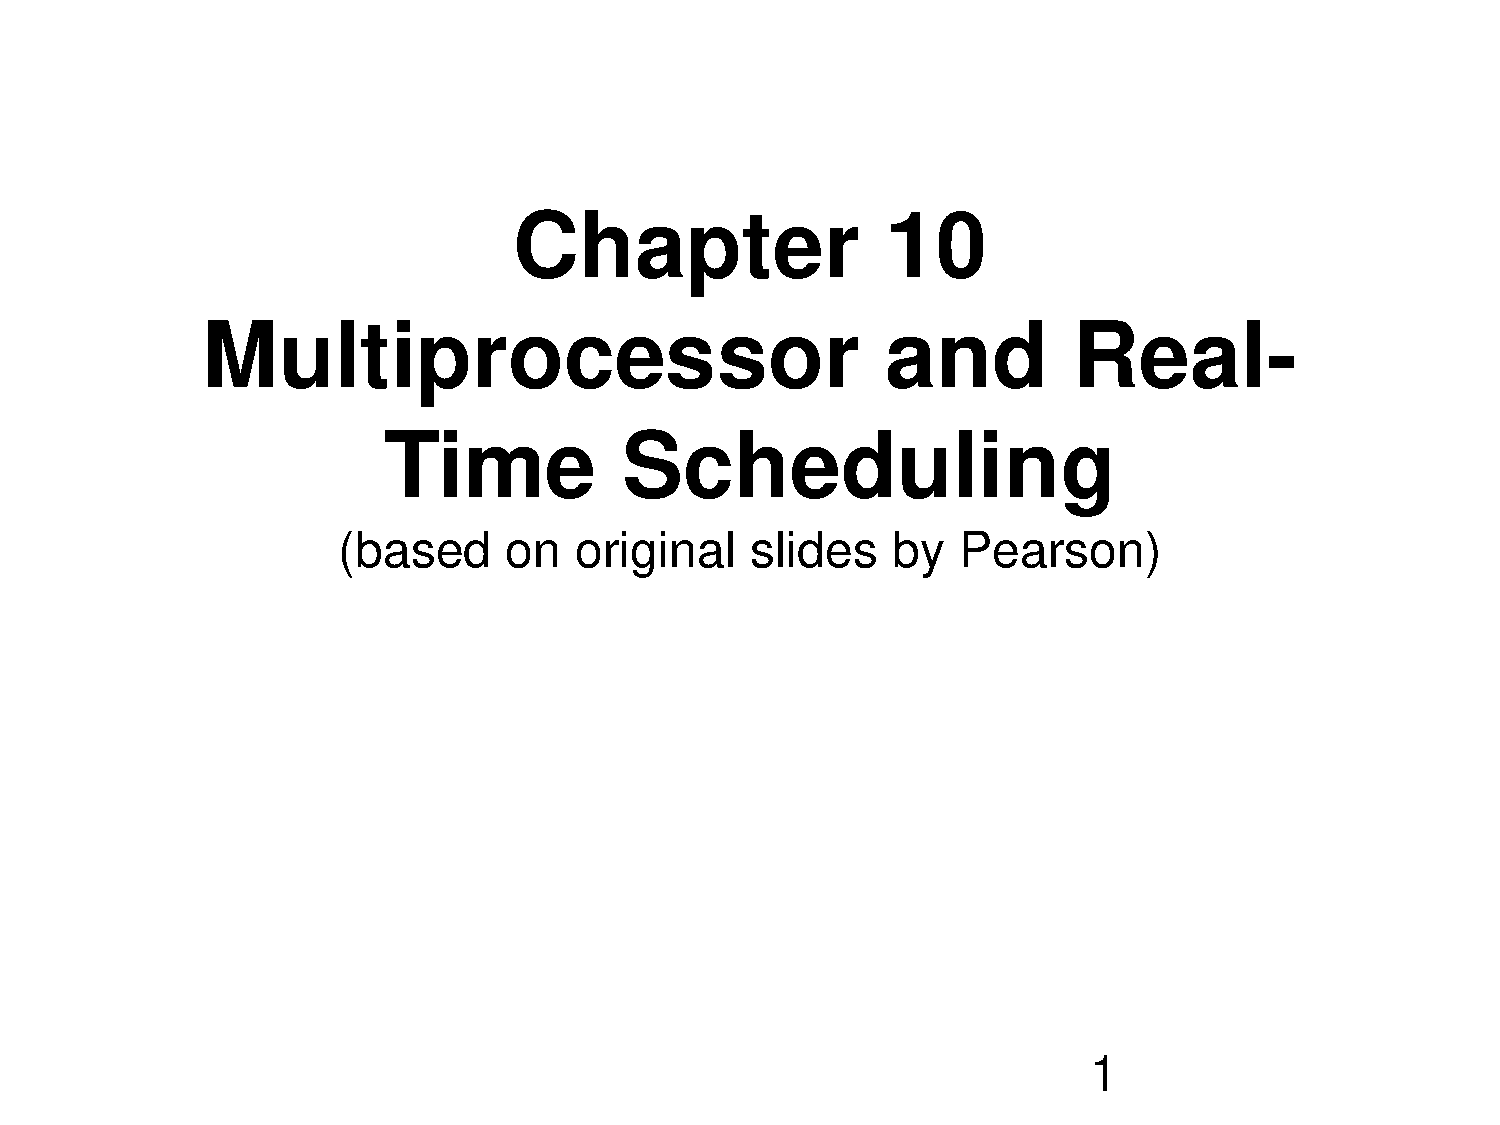
\includepdf[page=43]{10.pdf}
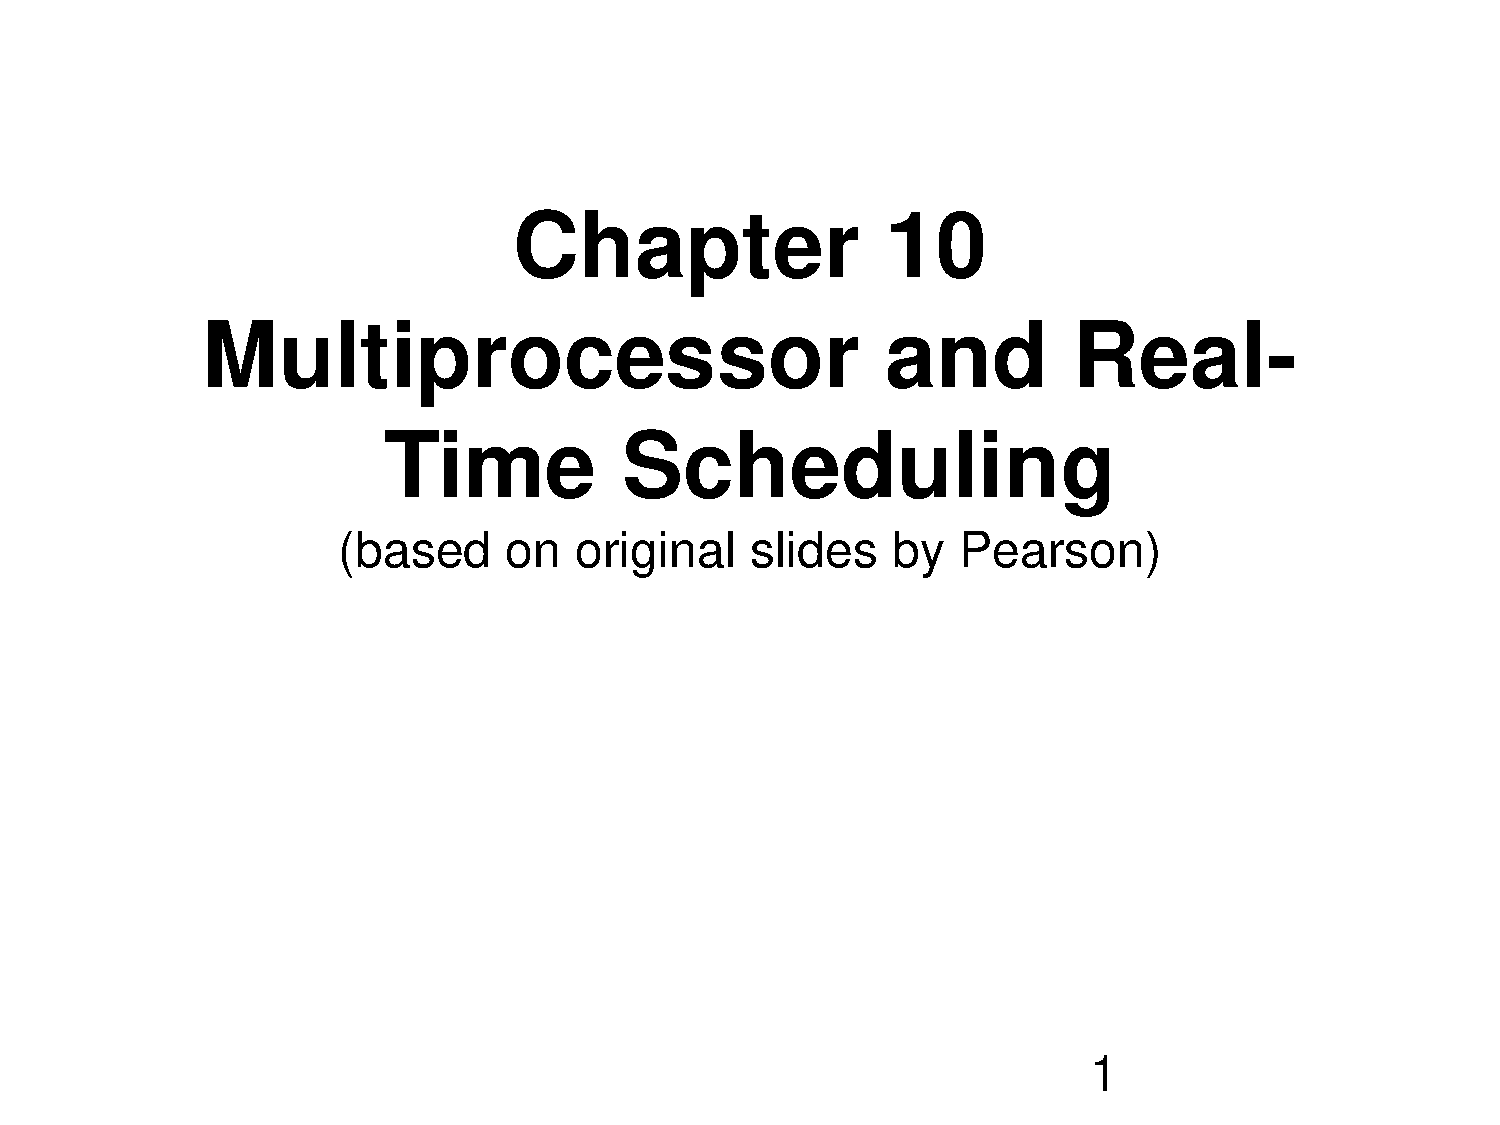
\includepdf[page=44]{10.pdf}
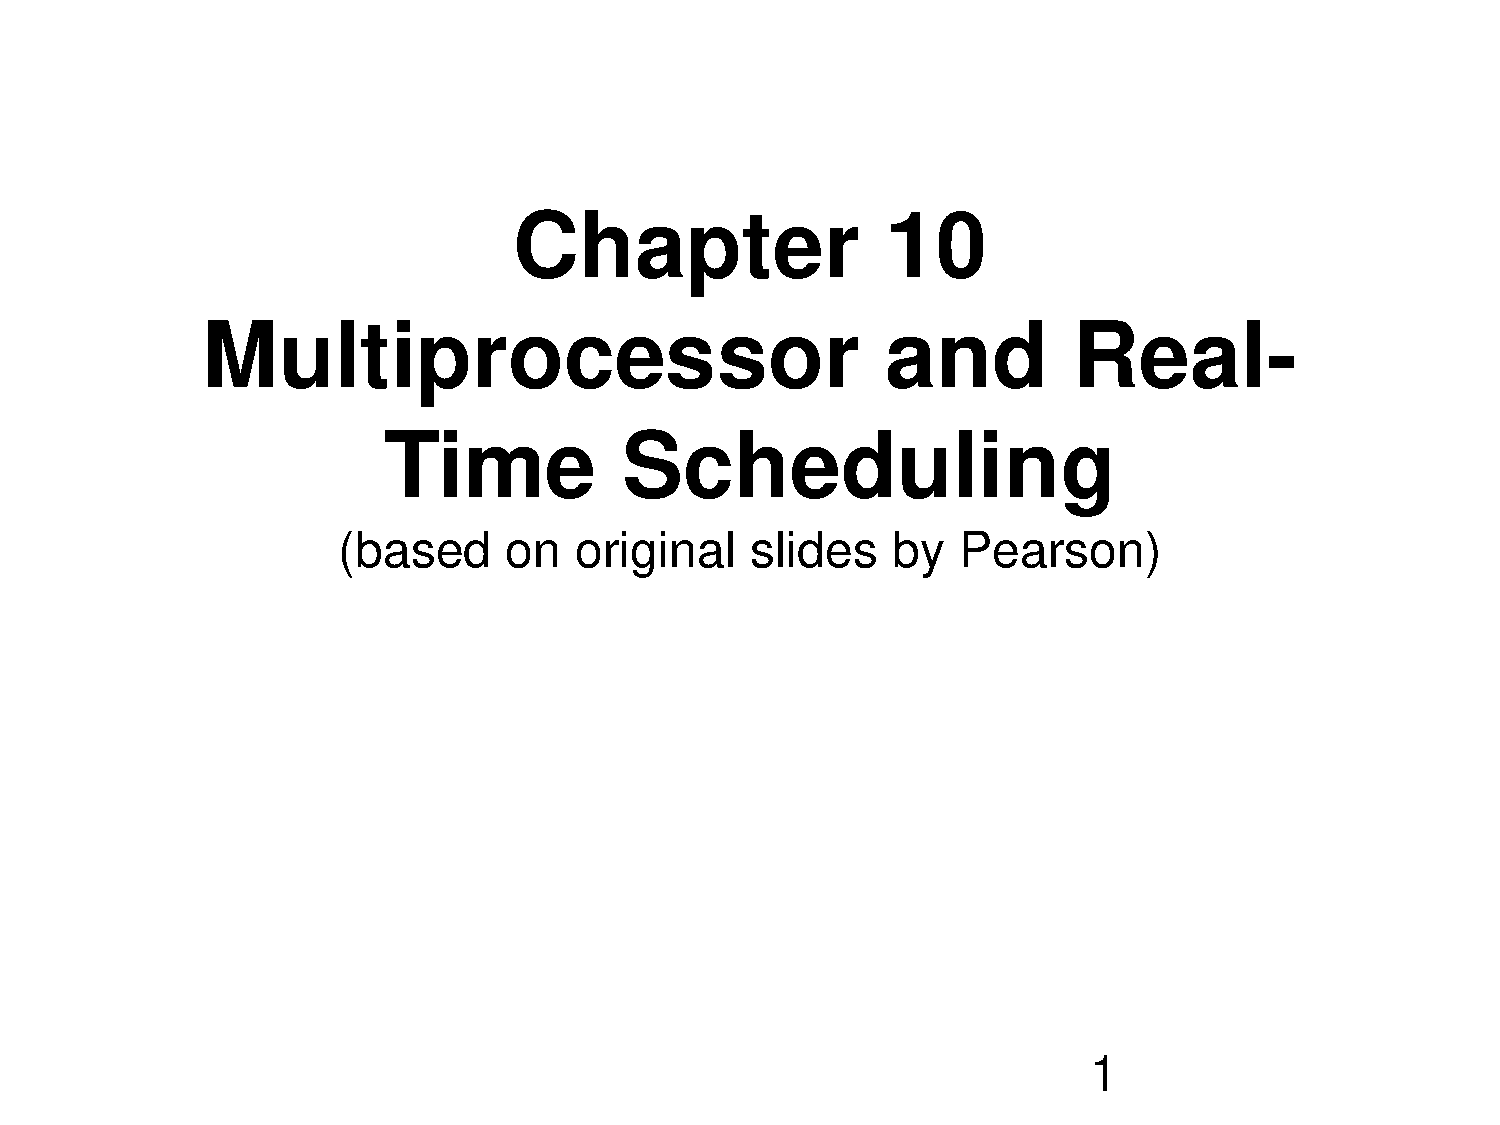
\includepdf[page=45]{10.pdf}
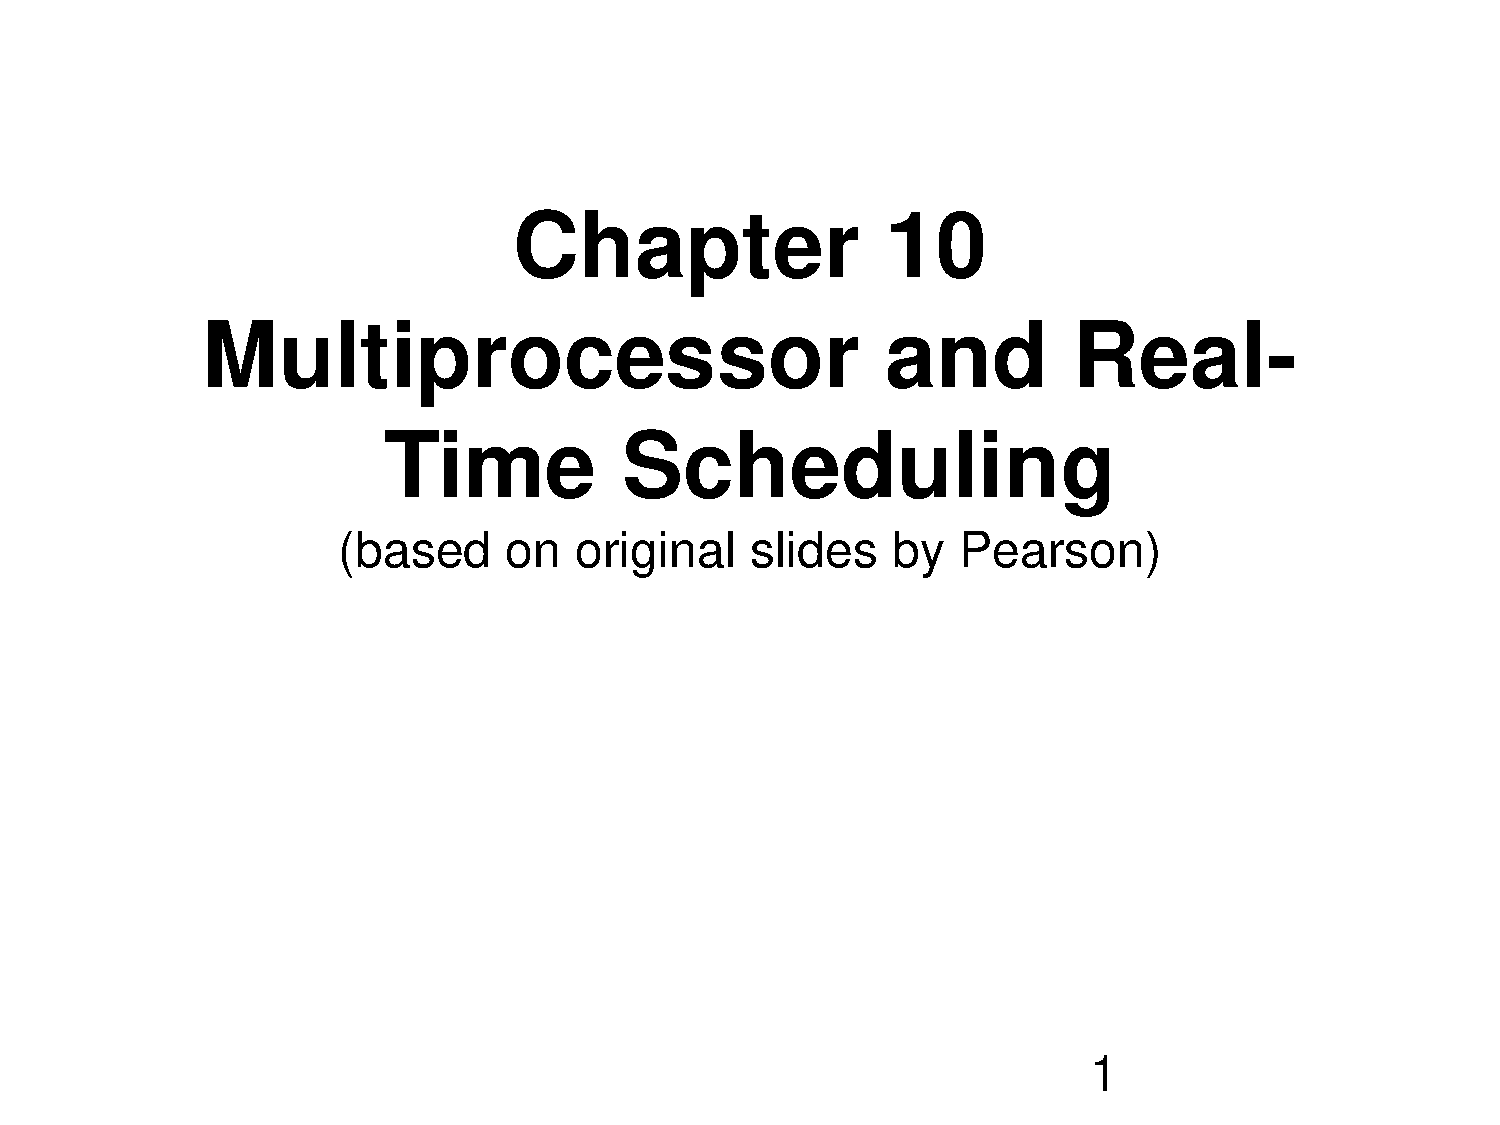
\includepdf[page=46]{10.pdf}
Here A attives every 20 ms and takes 10 ms and B arrives every 50m and takes 25 ms.

In the first option we have B1 miss its deadline because it doesnt finish before its ending deadline (see previous slide).

A similar thing happens when we make A the priority.

The final option is a preemptive strategy base in earliest deadline. When a process finishes we dont wait for the premption timer we straight up call the scheduler to immediately switch.
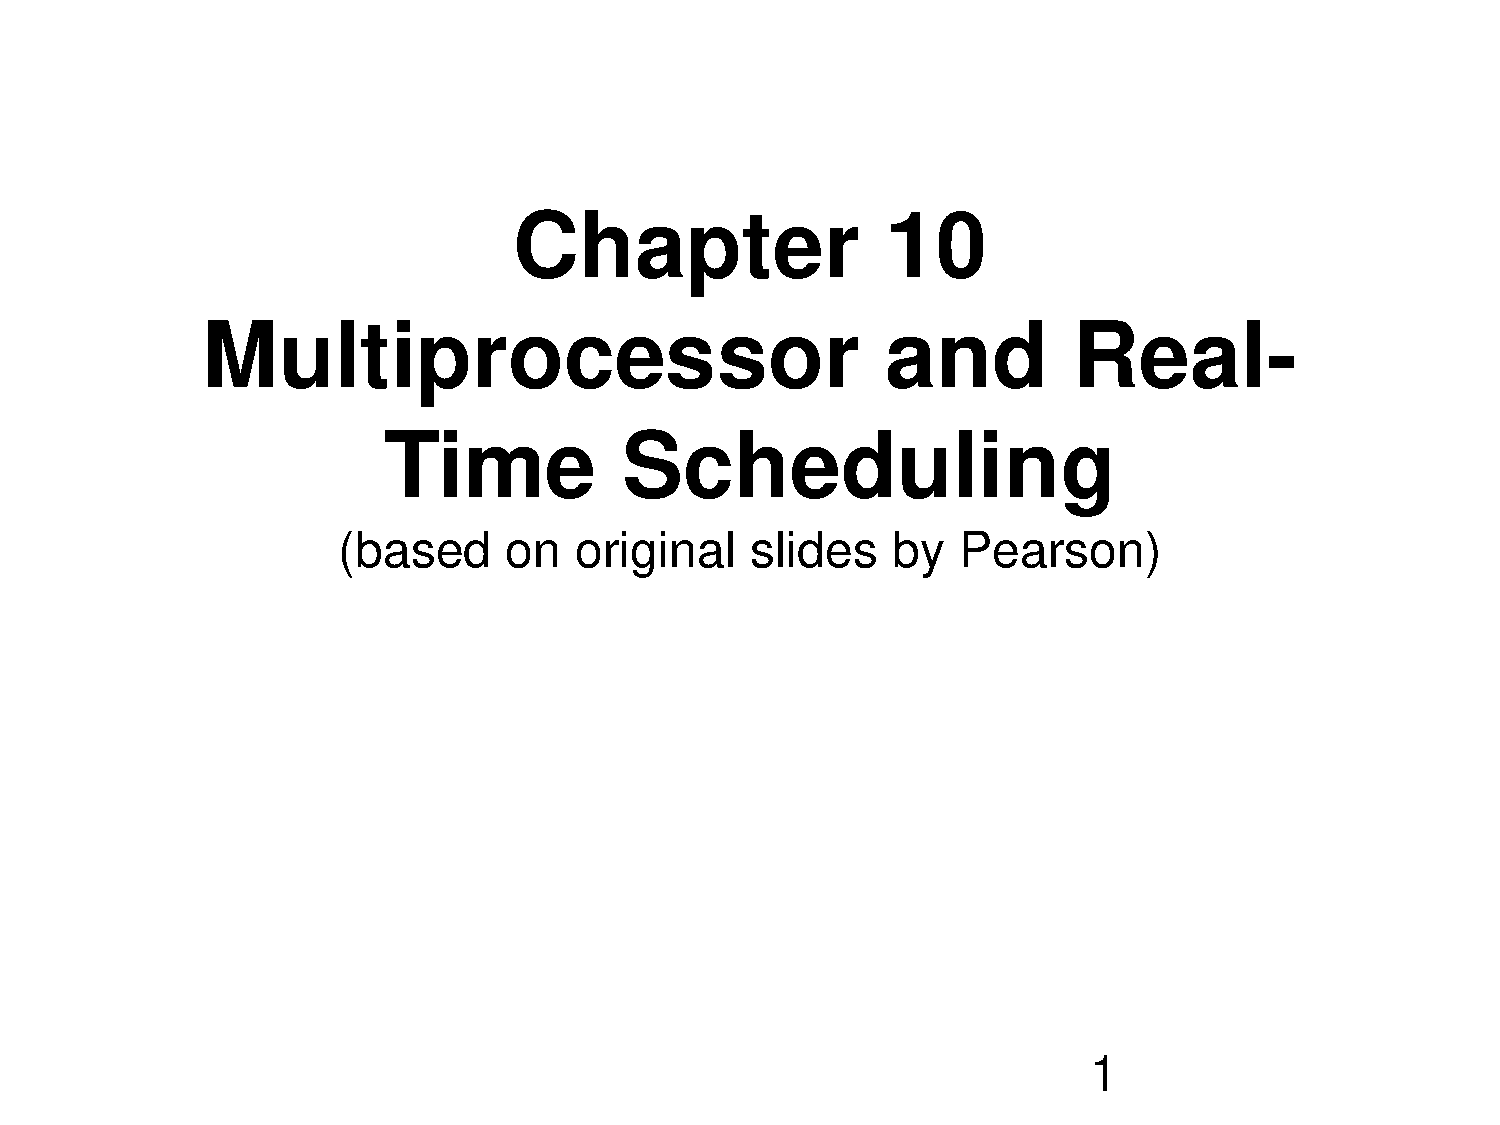
\includepdf[page=47]{10.pdf}
Here we use a starting deadline.
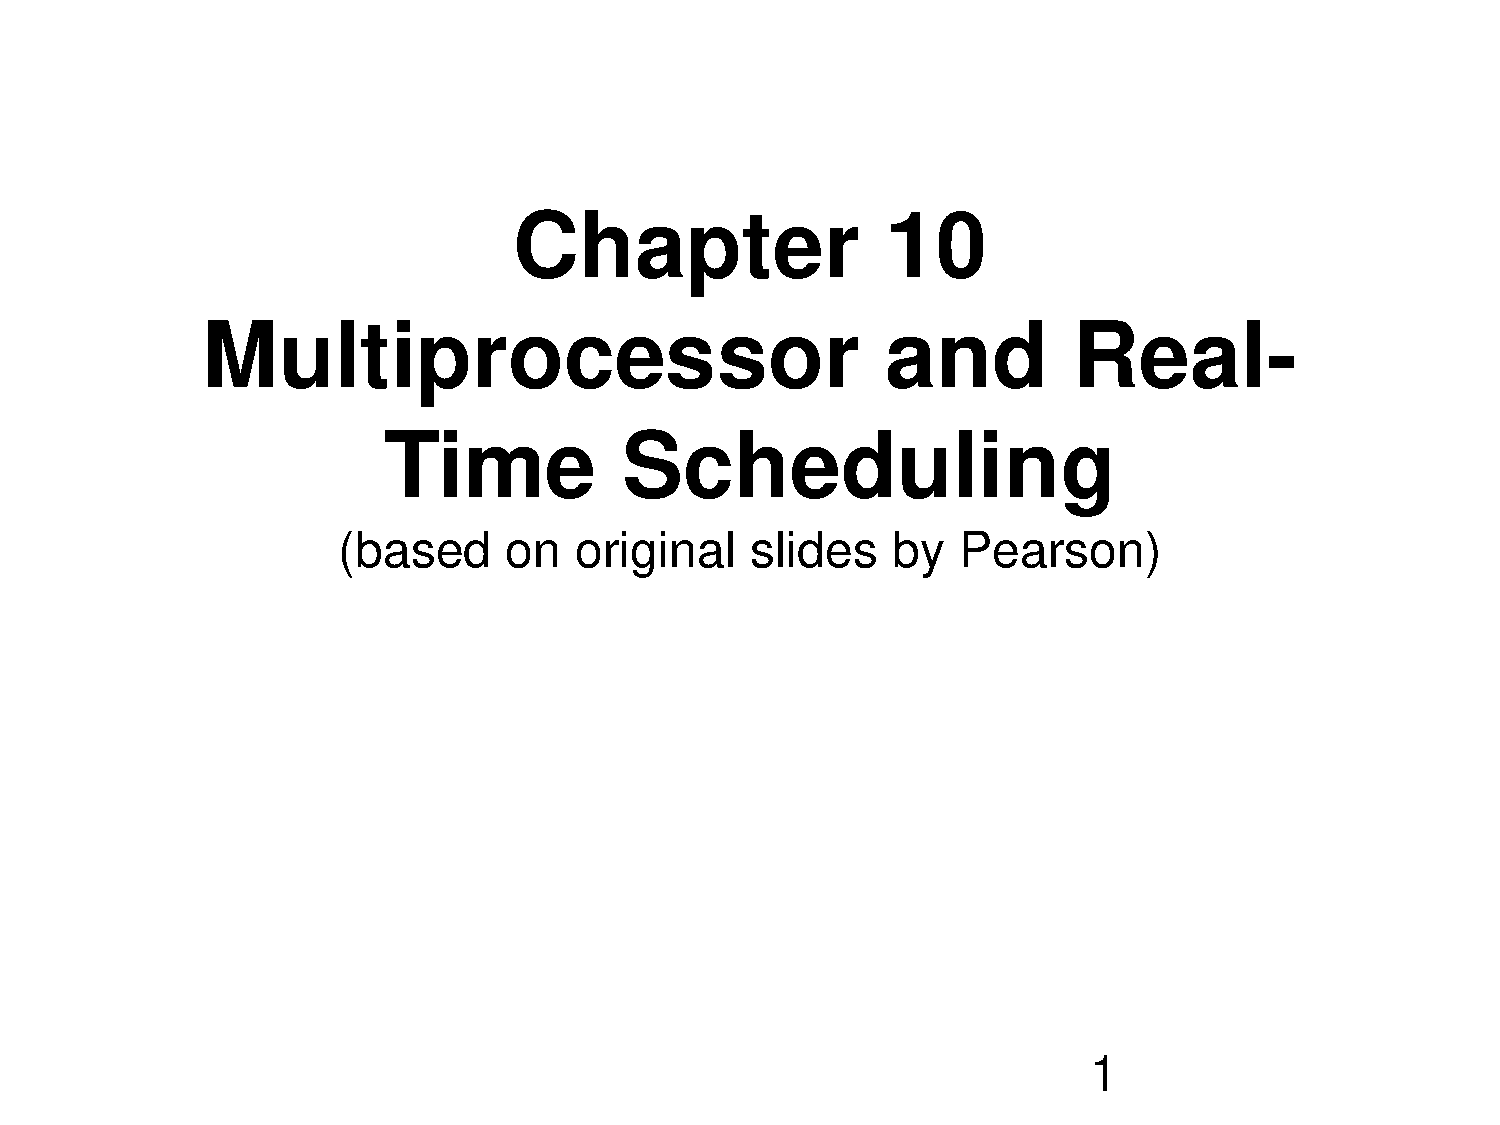
\includepdf[page=48]{10.pdf}
Once again a non preemptive strategy doesnt work.

We can make it work by scheduling tasks based on their starting deadline. We run them in that order and get no misses.
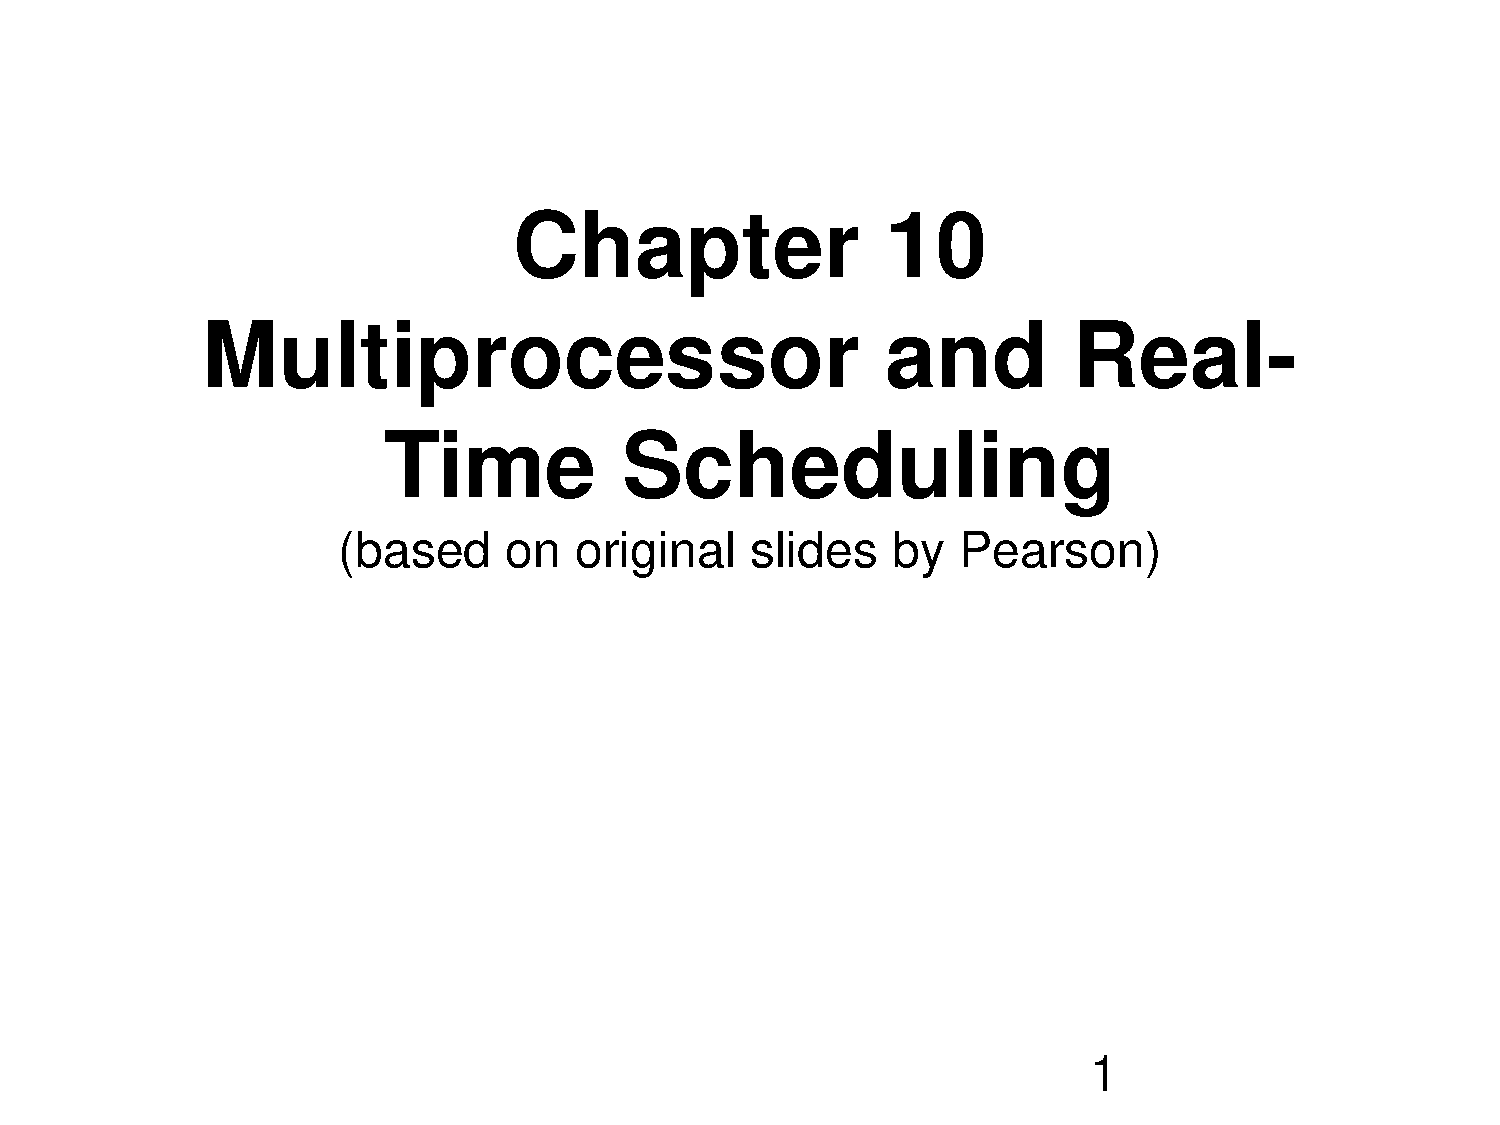
\includepdf[page=49]{10.pdf}

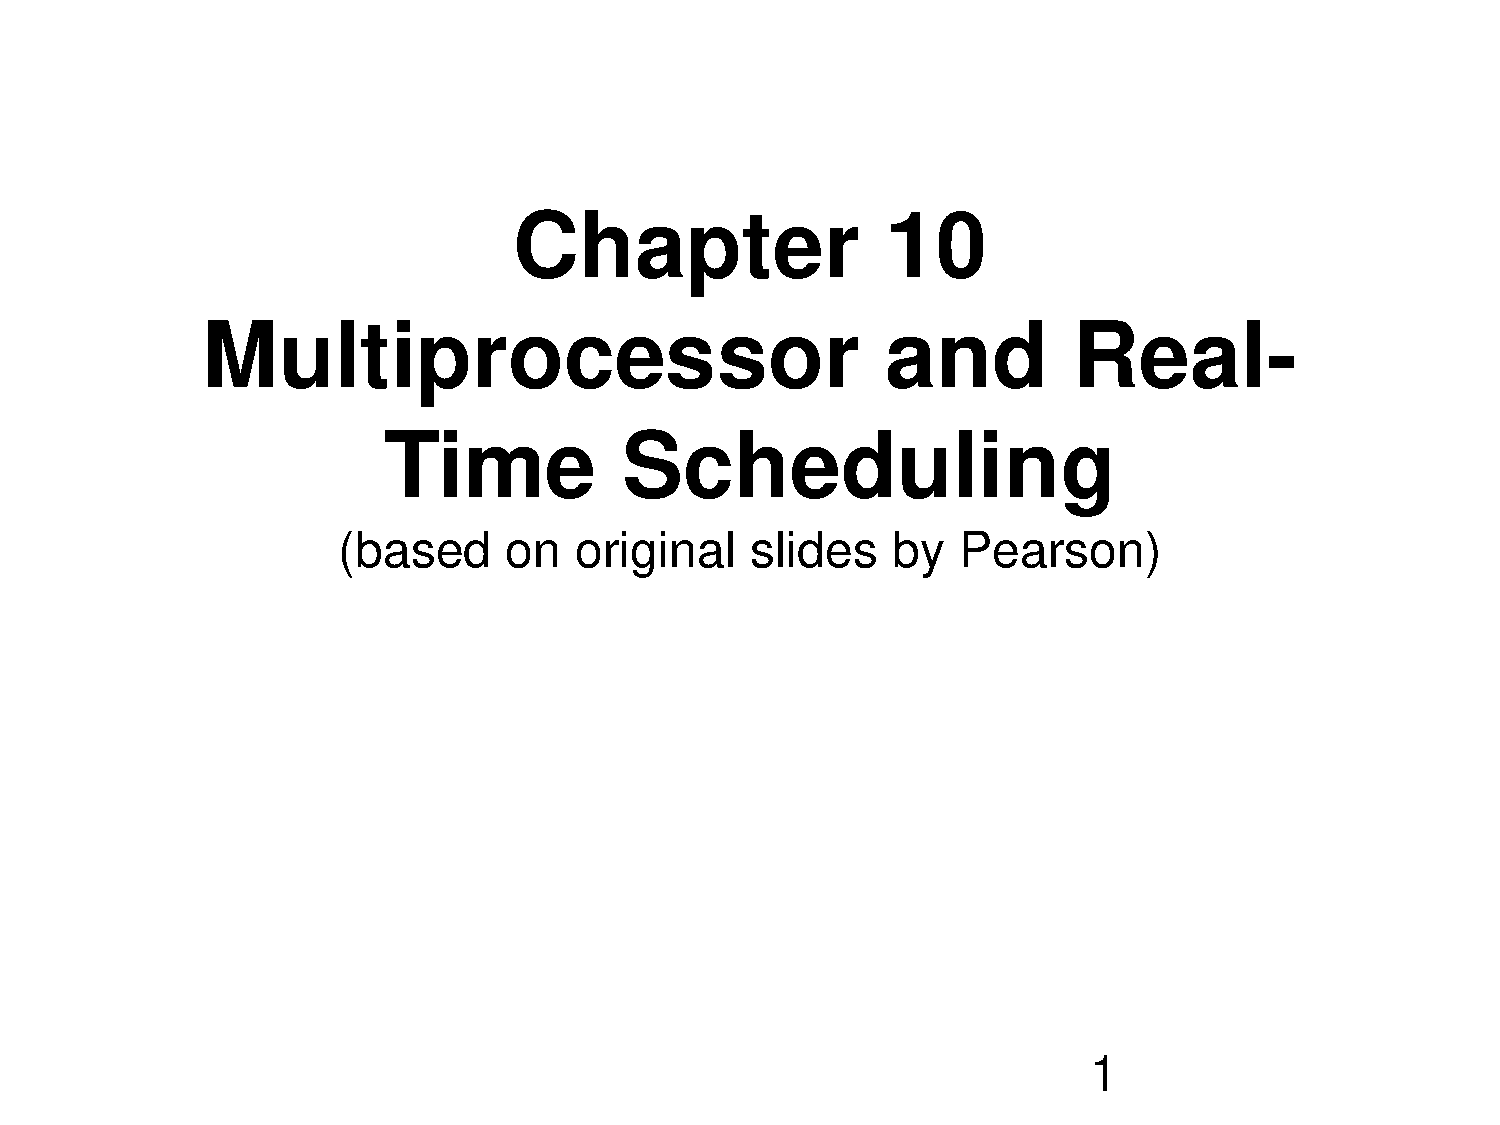
\includepdf[page=50]{10.pdf}
\includepdf[page=51]{10.pdf}
\includepdf[page=52]{10.pdf}
\includepdf[page=53]{10.pdf}
When a higher priority task is forced to wait for a lower priority task. Right before the lower priority task got preempted by the higher priority task it locked some resource. When the higher priority task wants to access that resource it must wait for the lower priority task to finish so that it can access that resource.
\includepdf[page=54]{10.pdf}
\includepdf[page=55]{10.pdf}
This is when lower priority tasks gain the priority of the tasks that are waiting on it. Assign a priority to a resource so that we know how urgently it is needed.






\end{document}
